% ---------------------------------------------------------------------------
%  Figure 1 panels (b) and (c) -- TEXT-FREE export for PowerPoint.
%
%  Every label / annotation has been removed (panel titles, axis labels,
%  "$v_t^{cand}$", "$R_{1,\eta}$", "$VO^T_1$", origin "0", correction symbols,
%  the union equations ...).  Geometry, colours and line weights are identical
%  to the in-paper TikZ figure, so text can be re-added by hand in PPT.
%
%  Build from this folder:
%    xelatex -jobname=fig1_b_clean  '\def\ONLYB{}% ---------------------------------------------------------------------------
%  Figure 1 panels (b) and (c) -- TEXT-FREE export for PowerPoint.
%
%  Every label / annotation has been removed (panel titles, axis labels,
%  "$v_t^{cand}$", "$R_{1,\eta}$", "$VO^T_1$", origin "0", correction symbols,
%  the union equations ...).  Geometry, colours and line weights are identical
%  to the in-paper TikZ figure, so text can be re-added by hand in PPT.
%
%  Build from this folder:
%    xelatex -jobname=fig1_b_clean  '\def\ONLYB{}% ---------------------------------------------------------------------------
%  Figure 1 panels (b) and (c) -- TEXT-FREE export for PowerPoint.
%
%  Every label / annotation has been removed (panel titles, axis labels,
%  "$v_t^{cand}$", "$R_{1,\eta}$", "$VO^T_1$", origin "0", correction symbols,
%  the union equations ...).  Geometry, colours and line weights are identical
%  to the in-paper TikZ figure, so text can be re-added by hand in PPT.
%
%  Build from this folder:
%    xelatex -jobname=fig1_b_clean  '\def\ONLYB{}% ---------------------------------------------------------------------------
%  Figure 1 panels (b) and (c) -- TEXT-FREE export for PowerPoint.
%
%  Every label / annotation has been removed (panel titles, axis labels,
%  "$v_t^{cand}$", "$R_{1,\eta}$", "$VO^T_1$", origin "0", correction symbols,
%  the union equations ...).  Geometry, colours and line weights are identical
%  to the in-paper TikZ figure, so text can be re-added by hand in PPT.
%
%  Build from this folder:
%    xelatex -jobname=fig1_b_clean  '\def\ONLYB{}\input{fig1_bc_clean.tex}'
%    xelatex -jobname=fig1_c_clean  '\def\ONLYC{}\input{fig1_bc_clean.tex}'
%    xelatex -jobname=fig1_bc_clean '\input{fig1_bc_clean.tex}'
% ---------------------------------------------------------------------------
\documentclass[tikz,border=2pt]{standalone}

\usepackage{tikz}
\usetikzlibrary{arrows.meta,positioning,calc}

\definecolor{pvoBlue}{HTML}{2F6FED}
\definecolor{pvoGreen}{HTML}{2AA876}
\definecolor{pvoRed}{HTML}{E05252}

\tikzset{
    line join=round, line cap=round,
    panel/.style={rounded corners=3pt, draw=black!20, line width=0.55pt},
    axis/.style={-{Latex[length=1.6mm]}, line width=0.7pt, draw=black!55},
    riskone/.style={line width=1.1pt, draw=pvoRed!88!black},
    risktwo/.style={line width=1.1pt, draw=pvoBlue!82!black},
    meanline/.style={line width=0.62pt, densely dashed},
    candidate/.style={-{Latex[length=1.8mm]}, line width=1.3pt, draw=black!80},
    accepted/.style={-{Latex[length=1.8mm]}, line width=1.3pt, draw=pvoGreen!80!black},
    correction/.style={-{Latex[length=1.4mm]}, line width=0.7pt, densely dashed, draw=black!55}
}

% --------------------------------------------------------------- panel (b) --
\newcommand{\panelB}{%
    \draw[panel] (-0.10,-0.12) rectangle (4.30,4.72);
    \begin{scope}[shift={(0.95,0.95)}, scale=0.85, shift={(-0.48,-0.52)}]
        \draw[axis] (0.48,0.52) -- (4.00,0.52);
        \draw[axis] (0.48,0.52) -- (0.48,3.82);

        % deterministic relative-velocity cone for obstacle 1
        \path[fill=pvoRed!13]
            (0.48,0.52) -- (3.82,3.86)
            .. controls (4.01,3.37) and (3.98,2.93) .. (3.69,2.53) -- cycle;
        \draw[riskone] (0.48,0.52) -- (3.82,3.86);
        \draw[riskone] (0.48,0.52) -- (3.69,2.53);
        \draw[riskone] (3.82,3.86) .. controls (4.01,3.37) and (3.98,2.93) .. (3.69,2.53);
        \draw[meanline, pvoRed!64] (0.48,0.52) -- (3.82,3.16);

        % deterministic relative-velocity cone for obstacle 2
        \path[fill=pvoBlue!11]
            (0.48,0.52) -- (3.84,2.42)
            .. controls (4.00,1.96) and (3.95,1.49) .. (3.76,1.08) -- cycle;
        \draw[risktwo] (0.48,0.52) -- (3.84,2.42);
        \draw[risktwo] (0.48,0.52) -- (3.76,1.08);
        \draw[risktwo] (3.84,2.42) .. controls (4.00,1.96) and (3.95,1.49) .. (3.76,1.08);
        \draw[meanline, pvoBlue!62] (0.48,0.52) -- (3.86,1.72);

        % candidate velocity / filtered velocity / correction
        \draw[candidate] (0.48,0.52) -- (2.95,2.13);
        \draw[accepted] (0.48,0.52) -- (1.58,3.45);
        \draw[correction] (2.95,2.13) -- (1.58,3.45);
    \end{scope}%
}

% --------------------------------------------------------------- panel (c) --
\newcommand{\panelC}{%
    \draw[panel] (-0.10,-0.12) rectangle (4.30,4.72);
    \begin{scope}[shift={(0.95,0.95)}, scale=0.85, shift={(-0.48,-0.52)}]
        \draw[axis] (0.48,0.52) -- (4.00,0.52);
        \draw[axis] (0.48,0.52) -- (0.48,3.82);

        % action-conditioned risk tube for obstacle 1
        \path[fill=pvoRed!13]
            (0.48,0.52)
            .. controls (1.52,1.72) and (2.13,3.25) .. (3.90,3.88)
            .. controls (3.95,3.33) and (3.88,2.88) .. (3.65,2.50)
            .. controls (2.72,2.35) and (1.64,1.02) .. (0.48,0.52) -- cycle;
        \draw[riskone]
            (0.48,0.52) .. controls (1.52,1.72) and (2.13,3.25) .. (3.90,3.88);
        \draw[riskone]
            (0.48,0.52) .. controls (1.64,1.02) and (2.72,2.35) .. (3.65,2.50);
        \draw[riskone] (3.90,3.88) .. controls (3.95,3.33) and (3.88,2.88) .. (3.65,2.50);
        \draw[meanline, pvoRed!65]
            (0.48,0.52) .. controls (1.72,1.35) and (2.38,2.73) .. (3.78,3.18);
        \draw[dotted, line width=0.75pt, pvoRed!62]
            (1.25,1.29) .. controls (1.86,1.88) and (2.46,2.92) .. (3.64,3.34);

        % action-conditioned risk tube for obstacle 2
        \path[fill=pvoBlue!11]
            (0.48,0.52)
            .. controls (1.45,0.88) and (2.17,2.25) .. (3.86,2.52)
            .. controls (4.00,2.06) and (3.96,1.52) .. (3.73,1.04)
            .. controls (2.55,1.32) and (1.53,0.63) .. (0.48,0.52) -- cycle;
        \draw[risktwo]
            (0.48,0.52) .. controls (1.45,0.88) and (2.17,2.25) .. (3.86,2.52);
        \draw[risktwo]
            (0.48,0.52) .. controls (1.53,0.63) and (2.55,1.32) .. (3.73,1.04);
        \draw[risktwo] (3.86,2.52) .. controls (4.00,2.06) and (3.96,1.52) .. (3.73,1.04);
        \draw[meanline, pvoBlue!64]
            (0.48,0.52) .. controls (1.55,0.77) and (2.30,1.78) .. (3.82,1.72);
        \draw[dotted, line width=0.75pt, pvoBlue!62]
            (1.13,0.81) .. controls (1.79,1.04) and (2.48,1.85) .. (3.60,1.91);

        % candidate velocity / filtered velocity / correction
        \draw[candidate] (0.48,0.52) -- (3.02,2.08);
        \draw[accepted] (0.48,0.52) -- (1.52,3.54);
        \draw[correction] (3.02,2.08) -- (1.52,3.54);
    \end{scope}%
}

\begin{document}
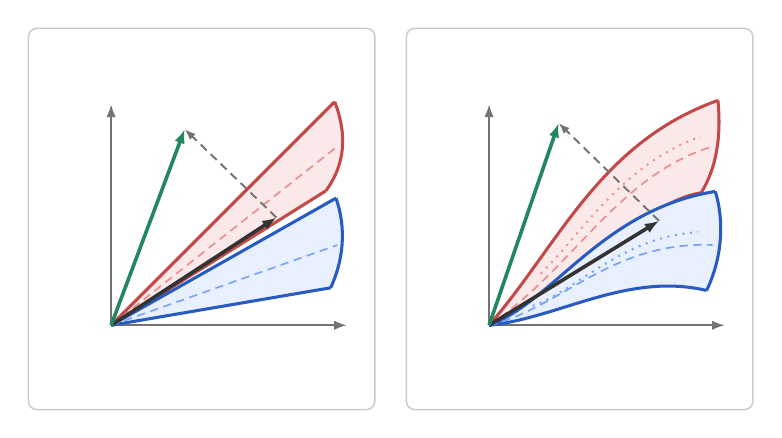
\begin{tikzpicture}
    \ifdefined\ONLYB
        \panelB
    \else
        \ifdefined\ONLYC
            \panelC
        \else
            \panelB
            \begin{scope}[xshift=4.80cm]
                \panelC
            \end{scope}
        \fi
    \fi
\end{tikzpicture}
\end{document}
'
%    xelatex -jobname=fig1_c_clean  '\def\ONLYC{}% ---------------------------------------------------------------------------
%  Figure 1 panels (b) and (c) -- TEXT-FREE export for PowerPoint.
%
%  Every label / annotation has been removed (panel titles, axis labels,
%  "$v_t^{cand}$", "$R_{1,\eta}$", "$VO^T_1$", origin "0", correction symbols,
%  the union equations ...).  Geometry, colours and line weights are identical
%  to the in-paper TikZ figure, so text can be re-added by hand in PPT.
%
%  Build from this folder:
%    xelatex -jobname=fig1_b_clean  '\def\ONLYB{}\input{fig1_bc_clean.tex}'
%    xelatex -jobname=fig1_c_clean  '\def\ONLYC{}\input{fig1_bc_clean.tex}'
%    xelatex -jobname=fig1_bc_clean '\input{fig1_bc_clean.tex}'
% ---------------------------------------------------------------------------
\documentclass[tikz,border=2pt]{standalone}

\usepackage{tikz}
\usetikzlibrary{arrows.meta,positioning,calc}

\definecolor{pvoBlue}{HTML}{2F6FED}
\definecolor{pvoGreen}{HTML}{2AA876}
\definecolor{pvoRed}{HTML}{E05252}

\tikzset{
    line join=round, line cap=round,
    panel/.style={rounded corners=3pt, draw=black!20, line width=0.55pt},
    axis/.style={-{Latex[length=1.6mm]}, line width=0.7pt, draw=black!55},
    riskone/.style={line width=1.1pt, draw=pvoRed!88!black},
    risktwo/.style={line width=1.1pt, draw=pvoBlue!82!black},
    meanline/.style={line width=0.62pt, densely dashed},
    candidate/.style={-{Latex[length=1.8mm]}, line width=1.3pt, draw=black!80},
    accepted/.style={-{Latex[length=1.8mm]}, line width=1.3pt, draw=pvoGreen!80!black},
    correction/.style={-{Latex[length=1.4mm]}, line width=0.7pt, densely dashed, draw=black!55}
}

% --------------------------------------------------------------- panel (b) --
\newcommand{\panelB}{%
    \draw[panel] (-0.10,-0.12) rectangle (4.30,4.72);
    \begin{scope}[shift={(0.95,0.95)}, scale=0.85, shift={(-0.48,-0.52)}]
        \draw[axis] (0.48,0.52) -- (4.00,0.52);
        \draw[axis] (0.48,0.52) -- (0.48,3.82);

        % deterministic relative-velocity cone for obstacle 1
        \path[fill=pvoRed!13]
            (0.48,0.52) -- (3.82,3.86)
            .. controls (4.01,3.37) and (3.98,2.93) .. (3.69,2.53) -- cycle;
        \draw[riskone] (0.48,0.52) -- (3.82,3.86);
        \draw[riskone] (0.48,0.52) -- (3.69,2.53);
        \draw[riskone] (3.82,3.86) .. controls (4.01,3.37) and (3.98,2.93) .. (3.69,2.53);
        \draw[meanline, pvoRed!64] (0.48,0.52) -- (3.82,3.16);

        % deterministic relative-velocity cone for obstacle 2
        \path[fill=pvoBlue!11]
            (0.48,0.52) -- (3.84,2.42)
            .. controls (4.00,1.96) and (3.95,1.49) .. (3.76,1.08) -- cycle;
        \draw[risktwo] (0.48,0.52) -- (3.84,2.42);
        \draw[risktwo] (0.48,0.52) -- (3.76,1.08);
        \draw[risktwo] (3.84,2.42) .. controls (4.00,1.96) and (3.95,1.49) .. (3.76,1.08);
        \draw[meanline, pvoBlue!62] (0.48,0.52) -- (3.86,1.72);

        % candidate velocity / filtered velocity / correction
        \draw[candidate] (0.48,0.52) -- (2.95,2.13);
        \draw[accepted] (0.48,0.52) -- (1.58,3.45);
        \draw[correction] (2.95,2.13) -- (1.58,3.45);
    \end{scope}%
}

% --------------------------------------------------------------- panel (c) --
\newcommand{\panelC}{%
    \draw[panel] (-0.10,-0.12) rectangle (4.30,4.72);
    \begin{scope}[shift={(0.95,0.95)}, scale=0.85, shift={(-0.48,-0.52)}]
        \draw[axis] (0.48,0.52) -- (4.00,0.52);
        \draw[axis] (0.48,0.52) -- (0.48,3.82);

        % action-conditioned risk tube for obstacle 1
        \path[fill=pvoRed!13]
            (0.48,0.52)
            .. controls (1.52,1.72) and (2.13,3.25) .. (3.90,3.88)
            .. controls (3.95,3.33) and (3.88,2.88) .. (3.65,2.50)
            .. controls (2.72,2.35) and (1.64,1.02) .. (0.48,0.52) -- cycle;
        \draw[riskone]
            (0.48,0.52) .. controls (1.52,1.72) and (2.13,3.25) .. (3.90,3.88);
        \draw[riskone]
            (0.48,0.52) .. controls (1.64,1.02) and (2.72,2.35) .. (3.65,2.50);
        \draw[riskone] (3.90,3.88) .. controls (3.95,3.33) and (3.88,2.88) .. (3.65,2.50);
        \draw[meanline, pvoRed!65]
            (0.48,0.52) .. controls (1.72,1.35) and (2.38,2.73) .. (3.78,3.18);
        \draw[dotted, line width=0.75pt, pvoRed!62]
            (1.25,1.29) .. controls (1.86,1.88) and (2.46,2.92) .. (3.64,3.34);

        % action-conditioned risk tube for obstacle 2
        \path[fill=pvoBlue!11]
            (0.48,0.52)
            .. controls (1.45,0.88) and (2.17,2.25) .. (3.86,2.52)
            .. controls (4.00,2.06) and (3.96,1.52) .. (3.73,1.04)
            .. controls (2.55,1.32) and (1.53,0.63) .. (0.48,0.52) -- cycle;
        \draw[risktwo]
            (0.48,0.52) .. controls (1.45,0.88) and (2.17,2.25) .. (3.86,2.52);
        \draw[risktwo]
            (0.48,0.52) .. controls (1.53,0.63) and (2.55,1.32) .. (3.73,1.04);
        \draw[risktwo] (3.86,2.52) .. controls (4.00,2.06) and (3.96,1.52) .. (3.73,1.04);
        \draw[meanline, pvoBlue!64]
            (0.48,0.52) .. controls (1.55,0.77) and (2.30,1.78) .. (3.82,1.72);
        \draw[dotted, line width=0.75pt, pvoBlue!62]
            (1.13,0.81) .. controls (1.79,1.04) and (2.48,1.85) .. (3.60,1.91);

        % candidate velocity / filtered velocity / correction
        \draw[candidate] (0.48,0.52) -- (3.02,2.08);
        \draw[accepted] (0.48,0.52) -- (1.52,3.54);
        \draw[correction] (3.02,2.08) -- (1.52,3.54);
    \end{scope}%
}

\begin{document}
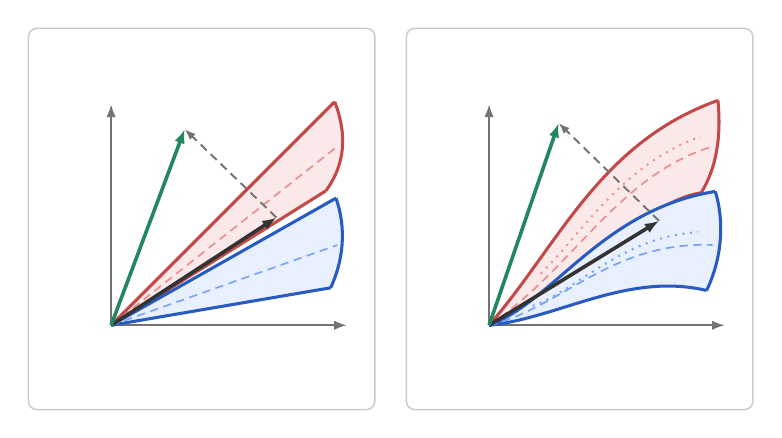
\begin{tikzpicture}
    \ifdefined\ONLYB
        \panelB
    \else
        \ifdefined\ONLYC
            \panelC
        \else
            \panelB
            \begin{scope}[xshift=4.80cm]
                \panelC
            \end{scope}
        \fi
    \fi
\end{tikzpicture}
\end{document}
'
%    xelatex -jobname=fig1_bc_clean '% ---------------------------------------------------------------------------
%  Figure 1 panels (b) and (c) -- TEXT-FREE export for PowerPoint.
%
%  Every label / annotation has been removed (panel titles, axis labels,
%  "$v_t^{cand}$", "$R_{1,\eta}$", "$VO^T_1$", origin "0", correction symbols,
%  the union equations ...).  Geometry, colours and line weights are identical
%  to the in-paper TikZ figure, so text can be re-added by hand in PPT.
%
%  Build from this folder:
%    xelatex -jobname=fig1_b_clean  '\def\ONLYB{}\input{fig1_bc_clean.tex}'
%    xelatex -jobname=fig1_c_clean  '\def\ONLYC{}\input{fig1_bc_clean.tex}'
%    xelatex -jobname=fig1_bc_clean '\input{fig1_bc_clean.tex}'
% ---------------------------------------------------------------------------
\documentclass[tikz,border=2pt]{standalone}

\usepackage{tikz}
\usetikzlibrary{arrows.meta,positioning,calc}

\definecolor{pvoBlue}{HTML}{2F6FED}
\definecolor{pvoGreen}{HTML}{2AA876}
\definecolor{pvoRed}{HTML}{E05252}

\tikzset{
    line join=round, line cap=round,
    panel/.style={rounded corners=3pt, draw=black!20, line width=0.55pt},
    axis/.style={-{Latex[length=1.6mm]}, line width=0.7pt, draw=black!55},
    riskone/.style={line width=1.1pt, draw=pvoRed!88!black},
    risktwo/.style={line width=1.1pt, draw=pvoBlue!82!black},
    meanline/.style={line width=0.62pt, densely dashed},
    candidate/.style={-{Latex[length=1.8mm]}, line width=1.3pt, draw=black!80},
    accepted/.style={-{Latex[length=1.8mm]}, line width=1.3pt, draw=pvoGreen!80!black},
    correction/.style={-{Latex[length=1.4mm]}, line width=0.7pt, densely dashed, draw=black!55}
}

% --------------------------------------------------------------- panel (b) --
\newcommand{\panelB}{%
    \draw[panel] (-0.10,-0.12) rectangle (4.30,4.72);
    \begin{scope}[shift={(0.95,0.95)}, scale=0.85, shift={(-0.48,-0.52)}]
        \draw[axis] (0.48,0.52) -- (4.00,0.52);
        \draw[axis] (0.48,0.52) -- (0.48,3.82);

        % deterministic relative-velocity cone for obstacle 1
        \path[fill=pvoRed!13]
            (0.48,0.52) -- (3.82,3.86)
            .. controls (4.01,3.37) and (3.98,2.93) .. (3.69,2.53) -- cycle;
        \draw[riskone] (0.48,0.52) -- (3.82,3.86);
        \draw[riskone] (0.48,0.52) -- (3.69,2.53);
        \draw[riskone] (3.82,3.86) .. controls (4.01,3.37) and (3.98,2.93) .. (3.69,2.53);
        \draw[meanline, pvoRed!64] (0.48,0.52) -- (3.82,3.16);

        % deterministic relative-velocity cone for obstacle 2
        \path[fill=pvoBlue!11]
            (0.48,0.52) -- (3.84,2.42)
            .. controls (4.00,1.96) and (3.95,1.49) .. (3.76,1.08) -- cycle;
        \draw[risktwo] (0.48,0.52) -- (3.84,2.42);
        \draw[risktwo] (0.48,0.52) -- (3.76,1.08);
        \draw[risktwo] (3.84,2.42) .. controls (4.00,1.96) and (3.95,1.49) .. (3.76,1.08);
        \draw[meanline, pvoBlue!62] (0.48,0.52) -- (3.86,1.72);

        % candidate velocity / filtered velocity / correction
        \draw[candidate] (0.48,0.52) -- (2.95,2.13);
        \draw[accepted] (0.48,0.52) -- (1.58,3.45);
        \draw[correction] (2.95,2.13) -- (1.58,3.45);
    \end{scope}%
}

% --------------------------------------------------------------- panel (c) --
\newcommand{\panelC}{%
    \draw[panel] (-0.10,-0.12) rectangle (4.30,4.72);
    \begin{scope}[shift={(0.95,0.95)}, scale=0.85, shift={(-0.48,-0.52)}]
        \draw[axis] (0.48,0.52) -- (4.00,0.52);
        \draw[axis] (0.48,0.52) -- (0.48,3.82);

        % action-conditioned risk tube for obstacle 1
        \path[fill=pvoRed!13]
            (0.48,0.52)
            .. controls (1.52,1.72) and (2.13,3.25) .. (3.90,3.88)
            .. controls (3.95,3.33) and (3.88,2.88) .. (3.65,2.50)
            .. controls (2.72,2.35) and (1.64,1.02) .. (0.48,0.52) -- cycle;
        \draw[riskone]
            (0.48,0.52) .. controls (1.52,1.72) and (2.13,3.25) .. (3.90,3.88);
        \draw[riskone]
            (0.48,0.52) .. controls (1.64,1.02) and (2.72,2.35) .. (3.65,2.50);
        \draw[riskone] (3.90,3.88) .. controls (3.95,3.33) and (3.88,2.88) .. (3.65,2.50);
        \draw[meanline, pvoRed!65]
            (0.48,0.52) .. controls (1.72,1.35) and (2.38,2.73) .. (3.78,3.18);
        \draw[dotted, line width=0.75pt, pvoRed!62]
            (1.25,1.29) .. controls (1.86,1.88) and (2.46,2.92) .. (3.64,3.34);

        % action-conditioned risk tube for obstacle 2
        \path[fill=pvoBlue!11]
            (0.48,0.52)
            .. controls (1.45,0.88) and (2.17,2.25) .. (3.86,2.52)
            .. controls (4.00,2.06) and (3.96,1.52) .. (3.73,1.04)
            .. controls (2.55,1.32) and (1.53,0.63) .. (0.48,0.52) -- cycle;
        \draw[risktwo]
            (0.48,0.52) .. controls (1.45,0.88) and (2.17,2.25) .. (3.86,2.52);
        \draw[risktwo]
            (0.48,0.52) .. controls (1.53,0.63) and (2.55,1.32) .. (3.73,1.04);
        \draw[risktwo] (3.86,2.52) .. controls (4.00,2.06) and (3.96,1.52) .. (3.73,1.04);
        \draw[meanline, pvoBlue!64]
            (0.48,0.52) .. controls (1.55,0.77) and (2.30,1.78) .. (3.82,1.72);
        \draw[dotted, line width=0.75pt, pvoBlue!62]
            (1.13,0.81) .. controls (1.79,1.04) and (2.48,1.85) .. (3.60,1.91);

        % candidate velocity / filtered velocity / correction
        \draw[candidate] (0.48,0.52) -- (3.02,2.08);
        \draw[accepted] (0.48,0.52) -- (1.52,3.54);
        \draw[correction] (3.02,2.08) -- (1.52,3.54);
    \end{scope}%
}

\begin{document}
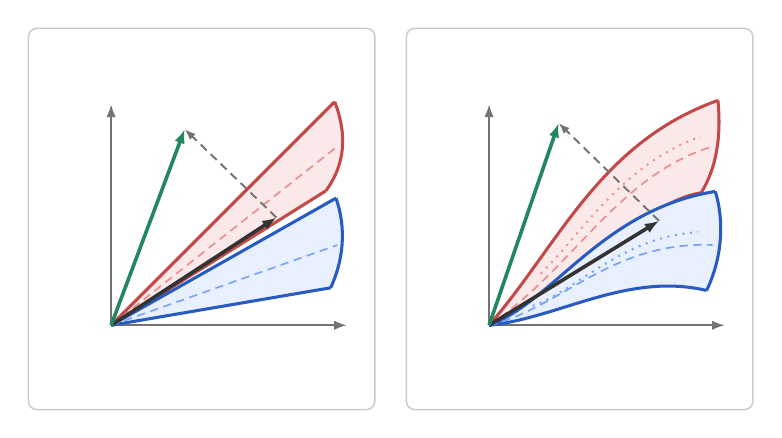
\begin{tikzpicture}
    \ifdefined\ONLYB
        \panelB
    \else
        \ifdefined\ONLYC
            \panelC
        \else
            \panelB
            \begin{scope}[xshift=4.80cm]
                \panelC
            \end{scope}
        \fi
    \fi
\end{tikzpicture}
\end{document}
'
% ---------------------------------------------------------------------------
\documentclass[tikz,border=2pt]{standalone}

\usepackage{tikz}
\usetikzlibrary{arrows.meta,positioning,calc}

\definecolor{pvoBlue}{HTML}{2F6FED}
\definecolor{pvoGreen}{HTML}{2AA876}
\definecolor{pvoRed}{HTML}{E05252}

\tikzset{
    line join=round, line cap=round,
    panel/.style={rounded corners=3pt, draw=black!20, line width=0.55pt},
    axis/.style={-{Latex[length=1.6mm]}, line width=0.7pt, draw=black!55},
    riskone/.style={line width=1.1pt, draw=pvoRed!88!black},
    risktwo/.style={line width=1.1pt, draw=pvoBlue!82!black},
    meanline/.style={line width=0.62pt, densely dashed},
    candidate/.style={-{Latex[length=1.8mm]}, line width=1.3pt, draw=black!80},
    accepted/.style={-{Latex[length=1.8mm]}, line width=1.3pt, draw=pvoGreen!80!black},
    correction/.style={-{Latex[length=1.4mm]}, line width=0.7pt, densely dashed, draw=black!55}
}

% --------------------------------------------------------------- panel (b) --
\newcommand{\panelB}{%
    \draw[panel] (-0.10,-0.12) rectangle (4.30,4.72);
    \begin{scope}[shift={(0.95,0.95)}, scale=0.85, shift={(-0.48,-0.52)}]
        \draw[axis] (0.48,0.52) -- (4.00,0.52);
        \draw[axis] (0.48,0.52) -- (0.48,3.82);

        % deterministic relative-velocity cone for obstacle 1
        \path[fill=pvoRed!13]
            (0.48,0.52) -- (3.82,3.86)
            .. controls (4.01,3.37) and (3.98,2.93) .. (3.69,2.53) -- cycle;
        \draw[riskone] (0.48,0.52) -- (3.82,3.86);
        \draw[riskone] (0.48,0.52) -- (3.69,2.53);
        \draw[riskone] (3.82,3.86) .. controls (4.01,3.37) and (3.98,2.93) .. (3.69,2.53);
        \draw[meanline, pvoRed!64] (0.48,0.52) -- (3.82,3.16);

        % deterministic relative-velocity cone for obstacle 2
        \path[fill=pvoBlue!11]
            (0.48,0.52) -- (3.84,2.42)
            .. controls (4.00,1.96) and (3.95,1.49) .. (3.76,1.08) -- cycle;
        \draw[risktwo] (0.48,0.52) -- (3.84,2.42);
        \draw[risktwo] (0.48,0.52) -- (3.76,1.08);
        \draw[risktwo] (3.84,2.42) .. controls (4.00,1.96) and (3.95,1.49) .. (3.76,1.08);
        \draw[meanline, pvoBlue!62] (0.48,0.52) -- (3.86,1.72);

        % candidate velocity / filtered velocity / correction
        \draw[candidate] (0.48,0.52) -- (2.95,2.13);
        \draw[accepted] (0.48,0.52) -- (1.58,3.45);
        \draw[correction] (2.95,2.13) -- (1.58,3.45);
    \end{scope}%
}

% --------------------------------------------------------------- panel (c) --
\newcommand{\panelC}{%
    \draw[panel] (-0.10,-0.12) rectangle (4.30,4.72);
    \begin{scope}[shift={(0.95,0.95)}, scale=0.85, shift={(-0.48,-0.52)}]
        \draw[axis] (0.48,0.52) -- (4.00,0.52);
        \draw[axis] (0.48,0.52) -- (0.48,3.82);

        % action-conditioned risk tube for obstacle 1
        \path[fill=pvoRed!13]
            (0.48,0.52)
            .. controls (1.52,1.72) and (2.13,3.25) .. (3.90,3.88)
            .. controls (3.95,3.33) and (3.88,2.88) .. (3.65,2.50)
            .. controls (2.72,2.35) and (1.64,1.02) .. (0.48,0.52) -- cycle;
        \draw[riskone]
            (0.48,0.52) .. controls (1.52,1.72) and (2.13,3.25) .. (3.90,3.88);
        \draw[riskone]
            (0.48,0.52) .. controls (1.64,1.02) and (2.72,2.35) .. (3.65,2.50);
        \draw[riskone] (3.90,3.88) .. controls (3.95,3.33) and (3.88,2.88) .. (3.65,2.50);
        \draw[meanline, pvoRed!65]
            (0.48,0.52) .. controls (1.72,1.35) and (2.38,2.73) .. (3.78,3.18);
        \draw[dotted, line width=0.75pt, pvoRed!62]
            (1.25,1.29) .. controls (1.86,1.88) and (2.46,2.92) .. (3.64,3.34);

        % action-conditioned risk tube for obstacle 2
        \path[fill=pvoBlue!11]
            (0.48,0.52)
            .. controls (1.45,0.88) and (2.17,2.25) .. (3.86,2.52)
            .. controls (4.00,2.06) and (3.96,1.52) .. (3.73,1.04)
            .. controls (2.55,1.32) and (1.53,0.63) .. (0.48,0.52) -- cycle;
        \draw[risktwo]
            (0.48,0.52) .. controls (1.45,0.88) and (2.17,2.25) .. (3.86,2.52);
        \draw[risktwo]
            (0.48,0.52) .. controls (1.53,0.63) and (2.55,1.32) .. (3.73,1.04);
        \draw[risktwo] (3.86,2.52) .. controls (4.00,2.06) and (3.96,1.52) .. (3.73,1.04);
        \draw[meanline, pvoBlue!64]
            (0.48,0.52) .. controls (1.55,0.77) and (2.30,1.78) .. (3.82,1.72);
        \draw[dotted, line width=0.75pt, pvoBlue!62]
            (1.13,0.81) .. controls (1.79,1.04) and (2.48,1.85) .. (3.60,1.91);

        % candidate velocity / filtered velocity / correction
        \draw[candidate] (0.48,0.52) -- (3.02,2.08);
        \draw[accepted] (0.48,0.52) -- (1.52,3.54);
        \draw[correction] (3.02,2.08) -- (1.52,3.54);
    \end{scope}%
}

\begin{document}
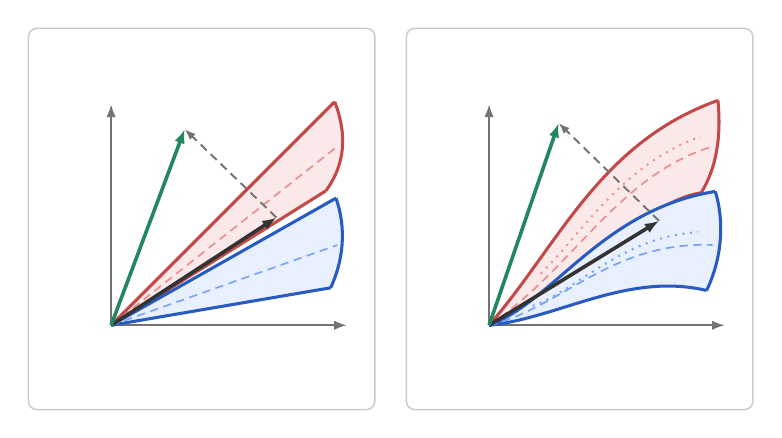
\begin{tikzpicture}
    \ifdefined\ONLYB
        \panelB
    \else
        \ifdefined\ONLYC
            \panelC
        \else
            \panelB
            \begin{scope}[xshift=4.80cm]
                \panelC
            \end{scope}
        \fi
    \fi
\end{tikzpicture}
\end{document}
'
%    xelatex -jobname=fig1_c_clean  '\def\ONLYC{}% ---------------------------------------------------------------------------
%  Figure 1 panels (b) and (c) -- TEXT-FREE export for PowerPoint.
%
%  Every label / annotation has been removed (panel titles, axis labels,
%  "$v_t^{cand}$", "$R_{1,\eta}$", "$VO^T_1$", origin "0", correction symbols,
%  the union equations ...).  Geometry, colours and line weights are identical
%  to the in-paper TikZ figure, so text can be re-added by hand in PPT.
%
%  Build from this folder:
%    xelatex -jobname=fig1_b_clean  '\def\ONLYB{}% ---------------------------------------------------------------------------
%  Figure 1 panels (b) and (c) -- TEXT-FREE export for PowerPoint.
%
%  Every label / annotation has been removed (panel titles, axis labels,
%  "$v_t^{cand}$", "$R_{1,\eta}$", "$VO^T_1$", origin "0", correction symbols,
%  the union equations ...).  Geometry, colours and line weights are identical
%  to the in-paper TikZ figure, so text can be re-added by hand in PPT.
%
%  Build from this folder:
%    xelatex -jobname=fig1_b_clean  '\def\ONLYB{}\input{fig1_bc_clean.tex}'
%    xelatex -jobname=fig1_c_clean  '\def\ONLYC{}\input{fig1_bc_clean.tex}'
%    xelatex -jobname=fig1_bc_clean '\input{fig1_bc_clean.tex}'
% ---------------------------------------------------------------------------
\documentclass[tikz,border=2pt]{standalone}

\usepackage{tikz}
\usetikzlibrary{arrows.meta,positioning,calc}

\definecolor{pvoBlue}{HTML}{2F6FED}
\definecolor{pvoGreen}{HTML}{2AA876}
\definecolor{pvoRed}{HTML}{E05252}

\tikzset{
    line join=round, line cap=round,
    panel/.style={rounded corners=3pt, draw=black!20, line width=0.55pt},
    axis/.style={-{Latex[length=1.6mm]}, line width=0.7pt, draw=black!55},
    riskone/.style={line width=1.1pt, draw=pvoRed!88!black},
    risktwo/.style={line width=1.1pt, draw=pvoBlue!82!black},
    meanline/.style={line width=0.62pt, densely dashed},
    candidate/.style={-{Latex[length=1.8mm]}, line width=1.3pt, draw=black!80},
    accepted/.style={-{Latex[length=1.8mm]}, line width=1.3pt, draw=pvoGreen!80!black},
    correction/.style={-{Latex[length=1.4mm]}, line width=0.7pt, densely dashed, draw=black!55}
}

% --------------------------------------------------------------- panel (b) --
\newcommand{\panelB}{%
    \draw[panel] (-0.10,-0.12) rectangle (4.30,4.72);
    \begin{scope}[shift={(0.95,0.95)}, scale=0.85, shift={(-0.48,-0.52)}]
        \draw[axis] (0.48,0.52) -- (4.00,0.52);
        \draw[axis] (0.48,0.52) -- (0.48,3.82);

        % deterministic relative-velocity cone for obstacle 1
        \path[fill=pvoRed!13]
            (0.48,0.52) -- (3.82,3.86)
            .. controls (4.01,3.37) and (3.98,2.93) .. (3.69,2.53) -- cycle;
        \draw[riskone] (0.48,0.52) -- (3.82,3.86);
        \draw[riskone] (0.48,0.52) -- (3.69,2.53);
        \draw[riskone] (3.82,3.86) .. controls (4.01,3.37) and (3.98,2.93) .. (3.69,2.53);
        \draw[meanline, pvoRed!64] (0.48,0.52) -- (3.82,3.16);

        % deterministic relative-velocity cone for obstacle 2
        \path[fill=pvoBlue!11]
            (0.48,0.52) -- (3.84,2.42)
            .. controls (4.00,1.96) and (3.95,1.49) .. (3.76,1.08) -- cycle;
        \draw[risktwo] (0.48,0.52) -- (3.84,2.42);
        \draw[risktwo] (0.48,0.52) -- (3.76,1.08);
        \draw[risktwo] (3.84,2.42) .. controls (4.00,1.96) and (3.95,1.49) .. (3.76,1.08);
        \draw[meanline, pvoBlue!62] (0.48,0.52) -- (3.86,1.72);

        % candidate velocity / filtered velocity / correction
        \draw[candidate] (0.48,0.52) -- (2.95,2.13);
        \draw[accepted] (0.48,0.52) -- (1.58,3.45);
        \draw[correction] (2.95,2.13) -- (1.58,3.45);
    \end{scope}%
}

% --------------------------------------------------------------- panel (c) --
\newcommand{\panelC}{%
    \draw[panel] (-0.10,-0.12) rectangle (4.30,4.72);
    \begin{scope}[shift={(0.95,0.95)}, scale=0.85, shift={(-0.48,-0.52)}]
        \draw[axis] (0.48,0.52) -- (4.00,0.52);
        \draw[axis] (0.48,0.52) -- (0.48,3.82);

        % action-conditioned risk tube for obstacle 1
        \path[fill=pvoRed!13]
            (0.48,0.52)
            .. controls (1.52,1.72) and (2.13,3.25) .. (3.90,3.88)
            .. controls (3.95,3.33) and (3.88,2.88) .. (3.65,2.50)
            .. controls (2.72,2.35) and (1.64,1.02) .. (0.48,0.52) -- cycle;
        \draw[riskone]
            (0.48,0.52) .. controls (1.52,1.72) and (2.13,3.25) .. (3.90,3.88);
        \draw[riskone]
            (0.48,0.52) .. controls (1.64,1.02) and (2.72,2.35) .. (3.65,2.50);
        \draw[riskone] (3.90,3.88) .. controls (3.95,3.33) and (3.88,2.88) .. (3.65,2.50);
        \draw[meanline, pvoRed!65]
            (0.48,0.52) .. controls (1.72,1.35) and (2.38,2.73) .. (3.78,3.18);
        \draw[dotted, line width=0.75pt, pvoRed!62]
            (1.25,1.29) .. controls (1.86,1.88) and (2.46,2.92) .. (3.64,3.34);

        % action-conditioned risk tube for obstacle 2
        \path[fill=pvoBlue!11]
            (0.48,0.52)
            .. controls (1.45,0.88) and (2.17,2.25) .. (3.86,2.52)
            .. controls (4.00,2.06) and (3.96,1.52) .. (3.73,1.04)
            .. controls (2.55,1.32) and (1.53,0.63) .. (0.48,0.52) -- cycle;
        \draw[risktwo]
            (0.48,0.52) .. controls (1.45,0.88) and (2.17,2.25) .. (3.86,2.52);
        \draw[risktwo]
            (0.48,0.52) .. controls (1.53,0.63) and (2.55,1.32) .. (3.73,1.04);
        \draw[risktwo] (3.86,2.52) .. controls (4.00,2.06) and (3.96,1.52) .. (3.73,1.04);
        \draw[meanline, pvoBlue!64]
            (0.48,0.52) .. controls (1.55,0.77) and (2.30,1.78) .. (3.82,1.72);
        \draw[dotted, line width=0.75pt, pvoBlue!62]
            (1.13,0.81) .. controls (1.79,1.04) and (2.48,1.85) .. (3.60,1.91);

        % candidate velocity / filtered velocity / correction
        \draw[candidate] (0.48,0.52) -- (3.02,2.08);
        \draw[accepted] (0.48,0.52) -- (1.52,3.54);
        \draw[correction] (3.02,2.08) -- (1.52,3.54);
    \end{scope}%
}

\begin{document}
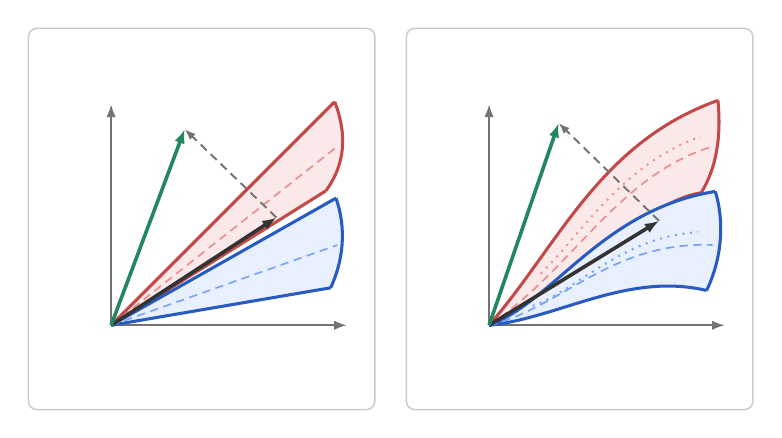
\begin{tikzpicture}
    \ifdefined\ONLYB
        \panelB
    \else
        \ifdefined\ONLYC
            \panelC
        \else
            \panelB
            \begin{scope}[xshift=4.80cm]
                \panelC
            \end{scope}
        \fi
    \fi
\end{tikzpicture}
\end{document}
'
%    xelatex -jobname=fig1_c_clean  '\def\ONLYC{}% ---------------------------------------------------------------------------
%  Figure 1 panels (b) and (c) -- TEXT-FREE export for PowerPoint.
%
%  Every label / annotation has been removed (panel titles, axis labels,
%  "$v_t^{cand}$", "$R_{1,\eta}$", "$VO^T_1$", origin "0", correction symbols,
%  the union equations ...).  Geometry, colours and line weights are identical
%  to the in-paper TikZ figure, so text can be re-added by hand in PPT.
%
%  Build from this folder:
%    xelatex -jobname=fig1_b_clean  '\def\ONLYB{}\input{fig1_bc_clean.tex}'
%    xelatex -jobname=fig1_c_clean  '\def\ONLYC{}\input{fig1_bc_clean.tex}'
%    xelatex -jobname=fig1_bc_clean '\input{fig1_bc_clean.tex}'
% ---------------------------------------------------------------------------
\documentclass[tikz,border=2pt]{standalone}

\usepackage{tikz}
\usetikzlibrary{arrows.meta,positioning,calc}

\definecolor{pvoBlue}{HTML}{2F6FED}
\definecolor{pvoGreen}{HTML}{2AA876}
\definecolor{pvoRed}{HTML}{E05252}

\tikzset{
    line join=round, line cap=round,
    panel/.style={rounded corners=3pt, draw=black!20, line width=0.55pt},
    axis/.style={-{Latex[length=1.6mm]}, line width=0.7pt, draw=black!55},
    riskone/.style={line width=1.1pt, draw=pvoRed!88!black},
    risktwo/.style={line width=1.1pt, draw=pvoBlue!82!black},
    meanline/.style={line width=0.62pt, densely dashed},
    candidate/.style={-{Latex[length=1.8mm]}, line width=1.3pt, draw=black!80},
    accepted/.style={-{Latex[length=1.8mm]}, line width=1.3pt, draw=pvoGreen!80!black},
    correction/.style={-{Latex[length=1.4mm]}, line width=0.7pt, densely dashed, draw=black!55}
}

% --------------------------------------------------------------- panel (b) --
\newcommand{\panelB}{%
    \draw[panel] (-0.10,-0.12) rectangle (4.30,4.72);
    \begin{scope}[shift={(0.95,0.95)}, scale=0.85, shift={(-0.48,-0.52)}]
        \draw[axis] (0.48,0.52) -- (4.00,0.52);
        \draw[axis] (0.48,0.52) -- (0.48,3.82);

        % deterministic relative-velocity cone for obstacle 1
        \path[fill=pvoRed!13]
            (0.48,0.52) -- (3.82,3.86)
            .. controls (4.01,3.37) and (3.98,2.93) .. (3.69,2.53) -- cycle;
        \draw[riskone] (0.48,0.52) -- (3.82,3.86);
        \draw[riskone] (0.48,0.52) -- (3.69,2.53);
        \draw[riskone] (3.82,3.86) .. controls (4.01,3.37) and (3.98,2.93) .. (3.69,2.53);
        \draw[meanline, pvoRed!64] (0.48,0.52) -- (3.82,3.16);

        % deterministic relative-velocity cone for obstacle 2
        \path[fill=pvoBlue!11]
            (0.48,0.52) -- (3.84,2.42)
            .. controls (4.00,1.96) and (3.95,1.49) .. (3.76,1.08) -- cycle;
        \draw[risktwo] (0.48,0.52) -- (3.84,2.42);
        \draw[risktwo] (0.48,0.52) -- (3.76,1.08);
        \draw[risktwo] (3.84,2.42) .. controls (4.00,1.96) and (3.95,1.49) .. (3.76,1.08);
        \draw[meanline, pvoBlue!62] (0.48,0.52) -- (3.86,1.72);

        % candidate velocity / filtered velocity / correction
        \draw[candidate] (0.48,0.52) -- (2.95,2.13);
        \draw[accepted] (0.48,0.52) -- (1.58,3.45);
        \draw[correction] (2.95,2.13) -- (1.58,3.45);
    \end{scope}%
}

% --------------------------------------------------------------- panel (c) --
\newcommand{\panelC}{%
    \draw[panel] (-0.10,-0.12) rectangle (4.30,4.72);
    \begin{scope}[shift={(0.95,0.95)}, scale=0.85, shift={(-0.48,-0.52)}]
        \draw[axis] (0.48,0.52) -- (4.00,0.52);
        \draw[axis] (0.48,0.52) -- (0.48,3.82);

        % action-conditioned risk tube for obstacle 1
        \path[fill=pvoRed!13]
            (0.48,0.52)
            .. controls (1.52,1.72) and (2.13,3.25) .. (3.90,3.88)
            .. controls (3.95,3.33) and (3.88,2.88) .. (3.65,2.50)
            .. controls (2.72,2.35) and (1.64,1.02) .. (0.48,0.52) -- cycle;
        \draw[riskone]
            (0.48,0.52) .. controls (1.52,1.72) and (2.13,3.25) .. (3.90,3.88);
        \draw[riskone]
            (0.48,0.52) .. controls (1.64,1.02) and (2.72,2.35) .. (3.65,2.50);
        \draw[riskone] (3.90,3.88) .. controls (3.95,3.33) and (3.88,2.88) .. (3.65,2.50);
        \draw[meanline, pvoRed!65]
            (0.48,0.52) .. controls (1.72,1.35) and (2.38,2.73) .. (3.78,3.18);
        \draw[dotted, line width=0.75pt, pvoRed!62]
            (1.25,1.29) .. controls (1.86,1.88) and (2.46,2.92) .. (3.64,3.34);

        % action-conditioned risk tube for obstacle 2
        \path[fill=pvoBlue!11]
            (0.48,0.52)
            .. controls (1.45,0.88) and (2.17,2.25) .. (3.86,2.52)
            .. controls (4.00,2.06) and (3.96,1.52) .. (3.73,1.04)
            .. controls (2.55,1.32) and (1.53,0.63) .. (0.48,0.52) -- cycle;
        \draw[risktwo]
            (0.48,0.52) .. controls (1.45,0.88) and (2.17,2.25) .. (3.86,2.52);
        \draw[risktwo]
            (0.48,0.52) .. controls (1.53,0.63) and (2.55,1.32) .. (3.73,1.04);
        \draw[risktwo] (3.86,2.52) .. controls (4.00,2.06) and (3.96,1.52) .. (3.73,1.04);
        \draw[meanline, pvoBlue!64]
            (0.48,0.52) .. controls (1.55,0.77) and (2.30,1.78) .. (3.82,1.72);
        \draw[dotted, line width=0.75pt, pvoBlue!62]
            (1.13,0.81) .. controls (1.79,1.04) and (2.48,1.85) .. (3.60,1.91);

        % candidate velocity / filtered velocity / correction
        \draw[candidate] (0.48,0.52) -- (3.02,2.08);
        \draw[accepted] (0.48,0.52) -- (1.52,3.54);
        \draw[correction] (3.02,2.08) -- (1.52,3.54);
    \end{scope}%
}

\begin{document}
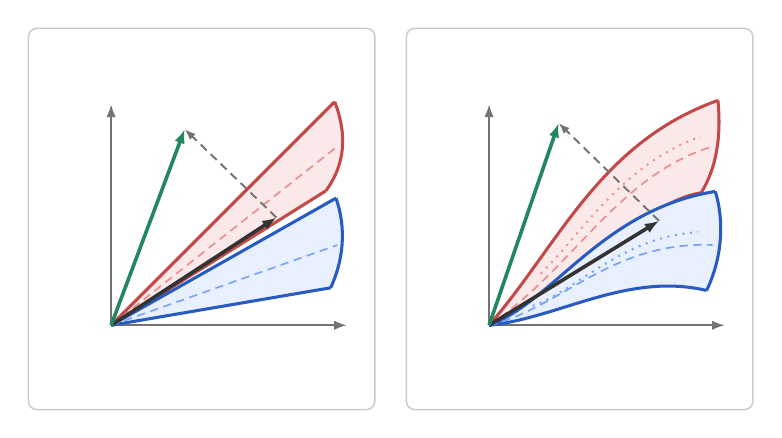
\begin{tikzpicture}
    \ifdefined\ONLYB
        \panelB
    \else
        \ifdefined\ONLYC
            \panelC
        \else
            \panelB
            \begin{scope}[xshift=4.80cm]
                \panelC
            \end{scope}
        \fi
    \fi
\end{tikzpicture}
\end{document}
'
%    xelatex -jobname=fig1_bc_clean '% ---------------------------------------------------------------------------
%  Figure 1 panels (b) and (c) -- TEXT-FREE export for PowerPoint.
%
%  Every label / annotation has been removed (panel titles, axis labels,
%  "$v_t^{cand}$", "$R_{1,\eta}$", "$VO^T_1$", origin "0", correction symbols,
%  the union equations ...).  Geometry, colours and line weights are identical
%  to the in-paper TikZ figure, so text can be re-added by hand in PPT.
%
%  Build from this folder:
%    xelatex -jobname=fig1_b_clean  '\def\ONLYB{}\input{fig1_bc_clean.tex}'
%    xelatex -jobname=fig1_c_clean  '\def\ONLYC{}\input{fig1_bc_clean.tex}'
%    xelatex -jobname=fig1_bc_clean '\input{fig1_bc_clean.tex}'
% ---------------------------------------------------------------------------
\documentclass[tikz,border=2pt]{standalone}

\usepackage{tikz}
\usetikzlibrary{arrows.meta,positioning,calc}

\definecolor{pvoBlue}{HTML}{2F6FED}
\definecolor{pvoGreen}{HTML}{2AA876}
\definecolor{pvoRed}{HTML}{E05252}

\tikzset{
    line join=round, line cap=round,
    panel/.style={rounded corners=3pt, draw=black!20, line width=0.55pt},
    axis/.style={-{Latex[length=1.6mm]}, line width=0.7pt, draw=black!55},
    riskone/.style={line width=1.1pt, draw=pvoRed!88!black},
    risktwo/.style={line width=1.1pt, draw=pvoBlue!82!black},
    meanline/.style={line width=0.62pt, densely dashed},
    candidate/.style={-{Latex[length=1.8mm]}, line width=1.3pt, draw=black!80},
    accepted/.style={-{Latex[length=1.8mm]}, line width=1.3pt, draw=pvoGreen!80!black},
    correction/.style={-{Latex[length=1.4mm]}, line width=0.7pt, densely dashed, draw=black!55}
}

% --------------------------------------------------------------- panel (b) --
\newcommand{\panelB}{%
    \draw[panel] (-0.10,-0.12) rectangle (4.30,4.72);
    \begin{scope}[shift={(0.95,0.95)}, scale=0.85, shift={(-0.48,-0.52)}]
        \draw[axis] (0.48,0.52) -- (4.00,0.52);
        \draw[axis] (0.48,0.52) -- (0.48,3.82);

        % deterministic relative-velocity cone for obstacle 1
        \path[fill=pvoRed!13]
            (0.48,0.52) -- (3.82,3.86)
            .. controls (4.01,3.37) and (3.98,2.93) .. (3.69,2.53) -- cycle;
        \draw[riskone] (0.48,0.52) -- (3.82,3.86);
        \draw[riskone] (0.48,0.52) -- (3.69,2.53);
        \draw[riskone] (3.82,3.86) .. controls (4.01,3.37) and (3.98,2.93) .. (3.69,2.53);
        \draw[meanline, pvoRed!64] (0.48,0.52) -- (3.82,3.16);

        % deterministic relative-velocity cone for obstacle 2
        \path[fill=pvoBlue!11]
            (0.48,0.52) -- (3.84,2.42)
            .. controls (4.00,1.96) and (3.95,1.49) .. (3.76,1.08) -- cycle;
        \draw[risktwo] (0.48,0.52) -- (3.84,2.42);
        \draw[risktwo] (0.48,0.52) -- (3.76,1.08);
        \draw[risktwo] (3.84,2.42) .. controls (4.00,1.96) and (3.95,1.49) .. (3.76,1.08);
        \draw[meanline, pvoBlue!62] (0.48,0.52) -- (3.86,1.72);

        % candidate velocity / filtered velocity / correction
        \draw[candidate] (0.48,0.52) -- (2.95,2.13);
        \draw[accepted] (0.48,0.52) -- (1.58,3.45);
        \draw[correction] (2.95,2.13) -- (1.58,3.45);
    \end{scope}%
}

% --------------------------------------------------------------- panel (c) --
\newcommand{\panelC}{%
    \draw[panel] (-0.10,-0.12) rectangle (4.30,4.72);
    \begin{scope}[shift={(0.95,0.95)}, scale=0.85, shift={(-0.48,-0.52)}]
        \draw[axis] (0.48,0.52) -- (4.00,0.52);
        \draw[axis] (0.48,0.52) -- (0.48,3.82);

        % action-conditioned risk tube for obstacle 1
        \path[fill=pvoRed!13]
            (0.48,0.52)
            .. controls (1.52,1.72) and (2.13,3.25) .. (3.90,3.88)
            .. controls (3.95,3.33) and (3.88,2.88) .. (3.65,2.50)
            .. controls (2.72,2.35) and (1.64,1.02) .. (0.48,0.52) -- cycle;
        \draw[riskone]
            (0.48,0.52) .. controls (1.52,1.72) and (2.13,3.25) .. (3.90,3.88);
        \draw[riskone]
            (0.48,0.52) .. controls (1.64,1.02) and (2.72,2.35) .. (3.65,2.50);
        \draw[riskone] (3.90,3.88) .. controls (3.95,3.33) and (3.88,2.88) .. (3.65,2.50);
        \draw[meanline, pvoRed!65]
            (0.48,0.52) .. controls (1.72,1.35) and (2.38,2.73) .. (3.78,3.18);
        \draw[dotted, line width=0.75pt, pvoRed!62]
            (1.25,1.29) .. controls (1.86,1.88) and (2.46,2.92) .. (3.64,3.34);

        % action-conditioned risk tube for obstacle 2
        \path[fill=pvoBlue!11]
            (0.48,0.52)
            .. controls (1.45,0.88) and (2.17,2.25) .. (3.86,2.52)
            .. controls (4.00,2.06) and (3.96,1.52) .. (3.73,1.04)
            .. controls (2.55,1.32) and (1.53,0.63) .. (0.48,0.52) -- cycle;
        \draw[risktwo]
            (0.48,0.52) .. controls (1.45,0.88) and (2.17,2.25) .. (3.86,2.52);
        \draw[risktwo]
            (0.48,0.52) .. controls (1.53,0.63) and (2.55,1.32) .. (3.73,1.04);
        \draw[risktwo] (3.86,2.52) .. controls (4.00,2.06) and (3.96,1.52) .. (3.73,1.04);
        \draw[meanline, pvoBlue!64]
            (0.48,0.52) .. controls (1.55,0.77) and (2.30,1.78) .. (3.82,1.72);
        \draw[dotted, line width=0.75pt, pvoBlue!62]
            (1.13,0.81) .. controls (1.79,1.04) and (2.48,1.85) .. (3.60,1.91);

        % candidate velocity / filtered velocity / correction
        \draw[candidate] (0.48,0.52) -- (3.02,2.08);
        \draw[accepted] (0.48,0.52) -- (1.52,3.54);
        \draw[correction] (3.02,2.08) -- (1.52,3.54);
    \end{scope}%
}

\begin{document}
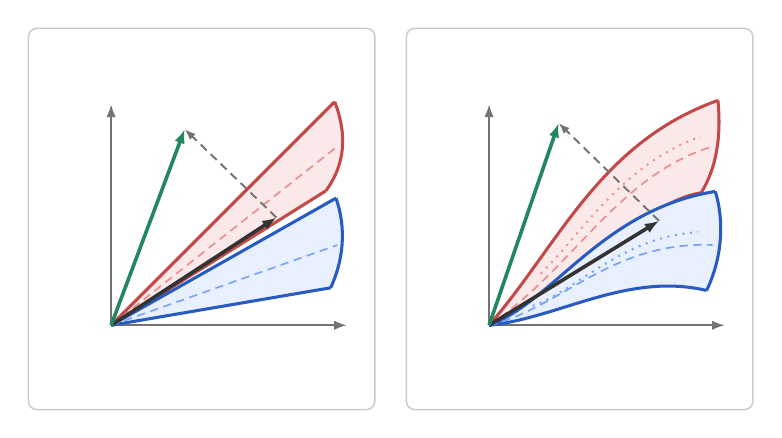
\begin{tikzpicture}
    \ifdefined\ONLYB
        \panelB
    \else
        \ifdefined\ONLYC
            \panelC
        \else
            \panelB
            \begin{scope}[xshift=4.80cm]
                \panelC
            \end{scope}
        \fi
    \fi
\end{tikzpicture}
\end{document}
'
% ---------------------------------------------------------------------------
\documentclass[tikz,border=2pt]{standalone}

\usepackage{tikz}
\usetikzlibrary{arrows.meta,positioning,calc}

\definecolor{pvoBlue}{HTML}{2F6FED}
\definecolor{pvoGreen}{HTML}{2AA876}
\definecolor{pvoRed}{HTML}{E05252}

\tikzset{
    line join=round, line cap=round,
    panel/.style={rounded corners=3pt, draw=black!20, line width=0.55pt},
    axis/.style={-{Latex[length=1.6mm]}, line width=0.7pt, draw=black!55},
    riskone/.style={line width=1.1pt, draw=pvoRed!88!black},
    risktwo/.style={line width=1.1pt, draw=pvoBlue!82!black},
    meanline/.style={line width=0.62pt, densely dashed},
    candidate/.style={-{Latex[length=1.8mm]}, line width=1.3pt, draw=black!80},
    accepted/.style={-{Latex[length=1.8mm]}, line width=1.3pt, draw=pvoGreen!80!black},
    correction/.style={-{Latex[length=1.4mm]}, line width=0.7pt, densely dashed, draw=black!55}
}

% --------------------------------------------------------------- panel (b) --
\newcommand{\panelB}{%
    \draw[panel] (-0.10,-0.12) rectangle (4.30,4.72);
    \begin{scope}[shift={(0.95,0.95)}, scale=0.85, shift={(-0.48,-0.52)}]
        \draw[axis] (0.48,0.52) -- (4.00,0.52);
        \draw[axis] (0.48,0.52) -- (0.48,3.82);

        % deterministic relative-velocity cone for obstacle 1
        \path[fill=pvoRed!13]
            (0.48,0.52) -- (3.82,3.86)
            .. controls (4.01,3.37) and (3.98,2.93) .. (3.69,2.53) -- cycle;
        \draw[riskone] (0.48,0.52) -- (3.82,3.86);
        \draw[riskone] (0.48,0.52) -- (3.69,2.53);
        \draw[riskone] (3.82,3.86) .. controls (4.01,3.37) and (3.98,2.93) .. (3.69,2.53);
        \draw[meanline, pvoRed!64] (0.48,0.52) -- (3.82,3.16);

        % deterministic relative-velocity cone for obstacle 2
        \path[fill=pvoBlue!11]
            (0.48,0.52) -- (3.84,2.42)
            .. controls (4.00,1.96) and (3.95,1.49) .. (3.76,1.08) -- cycle;
        \draw[risktwo] (0.48,0.52) -- (3.84,2.42);
        \draw[risktwo] (0.48,0.52) -- (3.76,1.08);
        \draw[risktwo] (3.84,2.42) .. controls (4.00,1.96) and (3.95,1.49) .. (3.76,1.08);
        \draw[meanline, pvoBlue!62] (0.48,0.52) -- (3.86,1.72);

        % candidate velocity / filtered velocity / correction
        \draw[candidate] (0.48,0.52) -- (2.95,2.13);
        \draw[accepted] (0.48,0.52) -- (1.58,3.45);
        \draw[correction] (2.95,2.13) -- (1.58,3.45);
    \end{scope}%
}

% --------------------------------------------------------------- panel (c) --
\newcommand{\panelC}{%
    \draw[panel] (-0.10,-0.12) rectangle (4.30,4.72);
    \begin{scope}[shift={(0.95,0.95)}, scale=0.85, shift={(-0.48,-0.52)}]
        \draw[axis] (0.48,0.52) -- (4.00,0.52);
        \draw[axis] (0.48,0.52) -- (0.48,3.82);

        % action-conditioned risk tube for obstacle 1
        \path[fill=pvoRed!13]
            (0.48,0.52)
            .. controls (1.52,1.72) and (2.13,3.25) .. (3.90,3.88)
            .. controls (3.95,3.33) and (3.88,2.88) .. (3.65,2.50)
            .. controls (2.72,2.35) and (1.64,1.02) .. (0.48,0.52) -- cycle;
        \draw[riskone]
            (0.48,0.52) .. controls (1.52,1.72) and (2.13,3.25) .. (3.90,3.88);
        \draw[riskone]
            (0.48,0.52) .. controls (1.64,1.02) and (2.72,2.35) .. (3.65,2.50);
        \draw[riskone] (3.90,3.88) .. controls (3.95,3.33) and (3.88,2.88) .. (3.65,2.50);
        \draw[meanline, pvoRed!65]
            (0.48,0.52) .. controls (1.72,1.35) and (2.38,2.73) .. (3.78,3.18);
        \draw[dotted, line width=0.75pt, pvoRed!62]
            (1.25,1.29) .. controls (1.86,1.88) and (2.46,2.92) .. (3.64,3.34);

        % action-conditioned risk tube for obstacle 2
        \path[fill=pvoBlue!11]
            (0.48,0.52)
            .. controls (1.45,0.88) and (2.17,2.25) .. (3.86,2.52)
            .. controls (4.00,2.06) and (3.96,1.52) .. (3.73,1.04)
            .. controls (2.55,1.32) and (1.53,0.63) .. (0.48,0.52) -- cycle;
        \draw[risktwo]
            (0.48,0.52) .. controls (1.45,0.88) and (2.17,2.25) .. (3.86,2.52);
        \draw[risktwo]
            (0.48,0.52) .. controls (1.53,0.63) and (2.55,1.32) .. (3.73,1.04);
        \draw[risktwo] (3.86,2.52) .. controls (4.00,2.06) and (3.96,1.52) .. (3.73,1.04);
        \draw[meanline, pvoBlue!64]
            (0.48,0.52) .. controls (1.55,0.77) and (2.30,1.78) .. (3.82,1.72);
        \draw[dotted, line width=0.75pt, pvoBlue!62]
            (1.13,0.81) .. controls (1.79,1.04) and (2.48,1.85) .. (3.60,1.91);

        % candidate velocity / filtered velocity / correction
        \draw[candidate] (0.48,0.52) -- (3.02,2.08);
        \draw[accepted] (0.48,0.52) -- (1.52,3.54);
        \draw[correction] (3.02,2.08) -- (1.52,3.54);
    \end{scope}%
}

\begin{document}
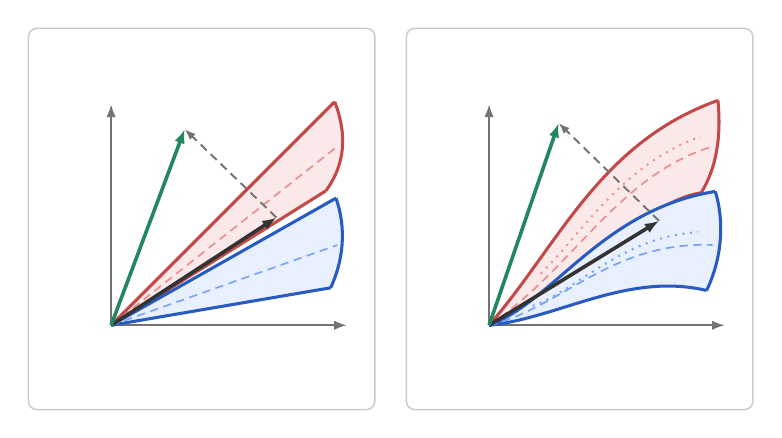
\begin{tikzpicture}
    \ifdefined\ONLYB
        \panelB
    \else
        \ifdefined\ONLYC
            \panelC
        \else
            \panelB
            \begin{scope}[xshift=4.80cm]
                \panelC
            \end{scope}
        \fi
    \fi
\end{tikzpicture}
\end{document}
'
%    xelatex -jobname=fig1_bc_clean '% ---------------------------------------------------------------------------
%  Figure 1 panels (b) and (c) -- TEXT-FREE export for PowerPoint.
%
%  Every label / annotation has been removed (panel titles, axis labels,
%  "$v_t^{cand}$", "$R_{1,\eta}$", "$VO^T_1$", origin "0", correction symbols,
%  the union equations ...).  Geometry, colours and line weights are identical
%  to the in-paper TikZ figure, so text can be re-added by hand in PPT.
%
%  Build from this folder:
%    xelatex -jobname=fig1_b_clean  '\def\ONLYB{}% ---------------------------------------------------------------------------
%  Figure 1 panels (b) and (c) -- TEXT-FREE export for PowerPoint.
%
%  Every label / annotation has been removed (panel titles, axis labels,
%  "$v_t^{cand}$", "$R_{1,\eta}$", "$VO^T_1$", origin "0", correction symbols,
%  the union equations ...).  Geometry, colours and line weights are identical
%  to the in-paper TikZ figure, so text can be re-added by hand in PPT.
%
%  Build from this folder:
%    xelatex -jobname=fig1_b_clean  '\def\ONLYB{}\input{fig1_bc_clean.tex}'
%    xelatex -jobname=fig1_c_clean  '\def\ONLYC{}\input{fig1_bc_clean.tex}'
%    xelatex -jobname=fig1_bc_clean '\input{fig1_bc_clean.tex}'
% ---------------------------------------------------------------------------
\documentclass[tikz,border=2pt]{standalone}

\usepackage{tikz}
\usetikzlibrary{arrows.meta,positioning,calc}

\definecolor{pvoBlue}{HTML}{2F6FED}
\definecolor{pvoGreen}{HTML}{2AA876}
\definecolor{pvoRed}{HTML}{E05252}

\tikzset{
    line join=round, line cap=round,
    panel/.style={rounded corners=3pt, draw=black!20, line width=0.55pt},
    axis/.style={-{Latex[length=1.6mm]}, line width=0.7pt, draw=black!55},
    riskone/.style={line width=1.1pt, draw=pvoRed!88!black},
    risktwo/.style={line width=1.1pt, draw=pvoBlue!82!black},
    meanline/.style={line width=0.62pt, densely dashed},
    candidate/.style={-{Latex[length=1.8mm]}, line width=1.3pt, draw=black!80},
    accepted/.style={-{Latex[length=1.8mm]}, line width=1.3pt, draw=pvoGreen!80!black},
    correction/.style={-{Latex[length=1.4mm]}, line width=0.7pt, densely dashed, draw=black!55}
}

% --------------------------------------------------------------- panel (b) --
\newcommand{\panelB}{%
    \draw[panel] (-0.10,-0.12) rectangle (4.30,4.72);
    \begin{scope}[shift={(0.95,0.95)}, scale=0.85, shift={(-0.48,-0.52)}]
        \draw[axis] (0.48,0.52) -- (4.00,0.52);
        \draw[axis] (0.48,0.52) -- (0.48,3.82);

        % deterministic relative-velocity cone for obstacle 1
        \path[fill=pvoRed!13]
            (0.48,0.52) -- (3.82,3.86)
            .. controls (4.01,3.37) and (3.98,2.93) .. (3.69,2.53) -- cycle;
        \draw[riskone] (0.48,0.52) -- (3.82,3.86);
        \draw[riskone] (0.48,0.52) -- (3.69,2.53);
        \draw[riskone] (3.82,3.86) .. controls (4.01,3.37) and (3.98,2.93) .. (3.69,2.53);
        \draw[meanline, pvoRed!64] (0.48,0.52) -- (3.82,3.16);

        % deterministic relative-velocity cone for obstacle 2
        \path[fill=pvoBlue!11]
            (0.48,0.52) -- (3.84,2.42)
            .. controls (4.00,1.96) and (3.95,1.49) .. (3.76,1.08) -- cycle;
        \draw[risktwo] (0.48,0.52) -- (3.84,2.42);
        \draw[risktwo] (0.48,0.52) -- (3.76,1.08);
        \draw[risktwo] (3.84,2.42) .. controls (4.00,1.96) and (3.95,1.49) .. (3.76,1.08);
        \draw[meanline, pvoBlue!62] (0.48,0.52) -- (3.86,1.72);

        % candidate velocity / filtered velocity / correction
        \draw[candidate] (0.48,0.52) -- (2.95,2.13);
        \draw[accepted] (0.48,0.52) -- (1.58,3.45);
        \draw[correction] (2.95,2.13) -- (1.58,3.45);
    \end{scope}%
}

% --------------------------------------------------------------- panel (c) --
\newcommand{\panelC}{%
    \draw[panel] (-0.10,-0.12) rectangle (4.30,4.72);
    \begin{scope}[shift={(0.95,0.95)}, scale=0.85, shift={(-0.48,-0.52)}]
        \draw[axis] (0.48,0.52) -- (4.00,0.52);
        \draw[axis] (0.48,0.52) -- (0.48,3.82);

        % action-conditioned risk tube for obstacle 1
        \path[fill=pvoRed!13]
            (0.48,0.52)
            .. controls (1.52,1.72) and (2.13,3.25) .. (3.90,3.88)
            .. controls (3.95,3.33) and (3.88,2.88) .. (3.65,2.50)
            .. controls (2.72,2.35) and (1.64,1.02) .. (0.48,0.52) -- cycle;
        \draw[riskone]
            (0.48,0.52) .. controls (1.52,1.72) and (2.13,3.25) .. (3.90,3.88);
        \draw[riskone]
            (0.48,0.52) .. controls (1.64,1.02) and (2.72,2.35) .. (3.65,2.50);
        \draw[riskone] (3.90,3.88) .. controls (3.95,3.33) and (3.88,2.88) .. (3.65,2.50);
        \draw[meanline, pvoRed!65]
            (0.48,0.52) .. controls (1.72,1.35) and (2.38,2.73) .. (3.78,3.18);
        \draw[dotted, line width=0.75pt, pvoRed!62]
            (1.25,1.29) .. controls (1.86,1.88) and (2.46,2.92) .. (3.64,3.34);

        % action-conditioned risk tube for obstacle 2
        \path[fill=pvoBlue!11]
            (0.48,0.52)
            .. controls (1.45,0.88) and (2.17,2.25) .. (3.86,2.52)
            .. controls (4.00,2.06) and (3.96,1.52) .. (3.73,1.04)
            .. controls (2.55,1.32) and (1.53,0.63) .. (0.48,0.52) -- cycle;
        \draw[risktwo]
            (0.48,0.52) .. controls (1.45,0.88) and (2.17,2.25) .. (3.86,2.52);
        \draw[risktwo]
            (0.48,0.52) .. controls (1.53,0.63) and (2.55,1.32) .. (3.73,1.04);
        \draw[risktwo] (3.86,2.52) .. controls (4.00,2.06) and (3.96,1.52) .. (3.73,1.04);
        \draw[meanline, pvoBlue!64]
            (0.48,0.52) .. controls (1.55,0.77) and (2.30,1.78) .. (3.82,1.72);
        \draw[dotted, line width=0.75pt, pvoBlue!62]
            (1.13,0.81) .. controls (1.79,1.04) and (2.48,1.85) .. (3.60,1.91);

        % candidate velocity / filtered velocity / correction
        \draw[candidate] (0.48,0.52) -- (3.02,2.08);
        \draw[accepted] (0.48,0.52) -- (1.52,3.54);
        \draw[correction] (3.02,2.08) -- (1.52,3.54);
    \end{scope}%
}

\begin{document}
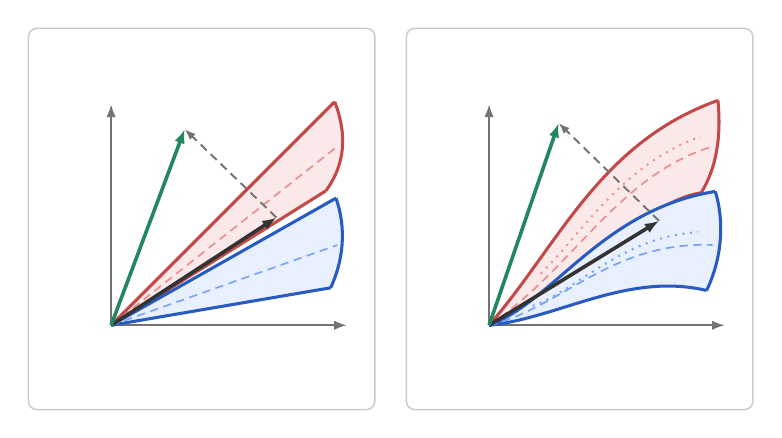
\begin{tikzpicture}
    \ifdefined\ONLYB
        \panelB
    \else
        \ifdefined\ONLYC
            \panelC
        \else
            \panelB
            \begin{scope}[xshift=4.80cm]
                \panelC
            \end{scope}
        \fi
    \fi
\end{tikzpicture}
\end{document}
'
%    xelatex -jobname=fig1_c_clean  '\def\ONLYC{}% ---------------------------------------------------------------------------
%  Figure 1 panels (b) and (c) -- TEXT-FREE export for PowerPoint.
%
%  Every label / annotation has been removed (panel titles, axis labels,
%  "$v_t^{cand}$", "$R_{1,\eta}$", "$VO^T_1$", origin "0", correction symbols,
%  the union equations ...).  Geometry, colours and line weights are identical
%  to the in-paper TikZ figure, so text can be re-added by hand in PPT.
%
%  Build from this folder:
%    xelatex -jobname=fig1_b_clean  '\def\ONLYB{}\input{fig1_bc_clean.tex}'
%    xelatex -jobname=fig1_c_clean  '\def\ONLYC{}\input{fig1_bc_clean.tex}'
%    xelatex -jobname=fig1_bc_clean '\input{fig1_bc_clean.tex}'
% ---------------------------------------------------------------------------
\documentclass[tikz,border=2pt]{standalone}

\usepackage{tikz}
\usetikzlibrary{arrows.meta,positioning,calc}

\definecolor{pvoBlue}{HTML}{2F6FED}
\definecolor{pvoGreen}{HTML}{2AA876}
\definecolor{pvoRed}{HTML}{E05252}

\tikzset{
    line join=round, line cap=round,
    panel/.style={rounded corners=3pt, draw=black!20, line width=0.55pt},
    axis/.style={-{Latex[length=1.6mm]}, line width=0.7pt, draw=black!55},
    riskone/.style={line width=1.1pt, draw=pvoRed!88!black},
    risktwo/.style={line width=1.1pt, draw=pvoBlue!82!black},
    meanline/.style={line width=0.62pt, densely dashed},
    candidate/.style={-{Latex[length=1.8mm]}, line width=1.3pt, draw=black!80},
    accepted/.style={-{Latex[length=1.8mm]}, line width=1.3pt, draw=pvoGreen!80!black},
    correction/.style={-{Latex[length=1.4mm]}, line width=0.7pt, densely dashed, draw=black!55}
}

% --------------------------------------------------------------- panel (b) --
\newcommand{\panelB}{%
    \draw[panel] (-0.10,-0.12) rectangle (4.30,4.72);
    \begin{scope}[shift={(0.95,0.95)}, scale=0.85, shift={(-0.48,-0.52)}]
        \draw[axis] (0.48,0.52) -- (4.00,0.52);
        \draw[axis] (0.48,0.52) -- (0.48,3.82);

        % deterministic relative-velocity cone for obstacle 1
        \path[fill=pvoRed!13]
            (0.48,0.52) -- (3.82,3.86)
            .. controls (4.01,3.37) and (3.98,2.93) .. (3.69,2.53) -- cycle;
        \draw[riskone] (0.48,0.52) -- (3.82,3.86);
        \draw[riskone] (0.48,0.52) -- (3.69,2.53);
        \draw[riskone] (3.82,3.86) .. controls (4.01,3.37) and (3.98,2.93) .. (3.69,2.53);
        \draw[meanline, pvoRed!64] (0.48,0.52) -- (3.82,3.16);

        % deterministic relative-velocity cone for obstacle 2
        \path[fill=pvoBlue!11]
            (0.48,0.52) -- (3.84,2.42)
            .. controls (4.00,1.96) and (3.95,1.49) .. (3.76,1.08) -- cycle;
        \draw[risktwo] (0.48,0.52) -- (3.84,2.42);
        \draw[risktwo] (0.48,0.52) -- (3.76,1.08);
        \draw[risktwo] (3.84,2.42) .. controls (4.00,1.96) and (3.95,1.49) .. (3.76,1.08);
        \draw[meanline, pvoBlue!62] (0.48,0.52) -- (3.86,1.72);

        % candidate velocity / filtered velocity / correction
        \draw[candidate] (0.48,0.52) -- (2.95,2.13);
        \draw[accepted] (0.48,0.52) -- (1.58,3.45);
        \draw[correction] (2.95,2.13) -- (1.58,3.45);
    \end{scope}%
}

% --------------------------------------------------------------- panel (c) --
\newcommand{\panelC}{%
    \draw[panel] (-0.10,-0.12) rectangle (4.30,4.72);
    \begin{scope}[shift={(0.95,0.95)}, scale=0.85, shift={(-0.48,-0.52)}]
        \draw[axis] (0.48,0.52) -- (4.00,0.52);
        \draw[axis] (0.48,0.52) -- (0.48,3.82);

        % action-conditioned risk tube for obstacle 1
        \path[fill=pvoRed!13]
            (0.48,0.52)
            .. controls (1.52,1.72) and (2.13,3.25) .. (3.90,3.88)
            .. controls (3.95,3.33) and (3.88,2.88) .. (3.65,2.50)
            .. controls (2.72,2.35) and (1.64,1.02) .. (0.48,0.52) -- cycle;
        \draw[riskone]
            (0.48,0.52) .. controls (1.52,1.72) and (2.13,3.25) .. (3.90,3.88);
        \draw[riskone]
            (0.48,0.52) .. controls (1.64,1.02) and (2.72,2.35) .. (3.65,2.50);
        \draw[riskone] (3.90,3.88) .. controls (3.95,3.33) and (3.88,2.88) .. (3.65,2.50);
        \draw[meanline, pvoRed!65]
            (0.48,0.52) .. controls (1.72,1.35) and (2.38,2.73) .. (3.78,3.18);
        \draw[dotted, line width=0.75pt, pvoRed!62]
            (1.25,1.29) .. controls (1.86,1.88) and (2.46,2.92) .. (3.64,3.34);

        % action-conditioned risk tube for obstacle 2
        \path[fill=pvoBlue!11]
            (0.48,0.52)
            .. controls (1.45,0.88) and (2.17,2.25) .. (3.86,2.52)
            .. controls (4.00,2.06) and (3.96,1.52) .. (3.73,1.04)
            .. controls (2.55,1.32) and (1.53,0.63) .. (0.48,0.52) -- cycle;
        \draw[risktwo]
            (0.48,0.52) .. controls (1.45,0.88) and (2.17,2.25) .. (3.86,2.52);
        \draw[risktwo]
            (0.48,0.52) .. controls (1.53,0.63) and (2.55,1.32) .. (3.73,1.04);
        \draw[risktwo] (3.86,2.52) .. controls (4.00,2.06) and (3.96,1.52) .. (3.73,1.04);
        \draw[meanline, pvoBlue!64]
            (0.48,0.52) .. controls (1.55,0.77) and (2.30,1.78) .. (3.82,1.72);
        \draw[dotted, line width=0.75pt, pvoBlue!62]
            (1.13,0.81) .. controls (1.79,1.04) and (2.48,1.85) .. (3.60,1.91);

        % candidate velocity / filtered velocity / correction
        \draw[candidate] (0.48,0.52) -- (3.02,2.08);
        \draw[accepted] (0.48,0.52) -- (1.52,3.54);
        \draw[correction] (3.02,2.08) -- (1.52,3.54);
    \end{scope}%
}

\begin{document}
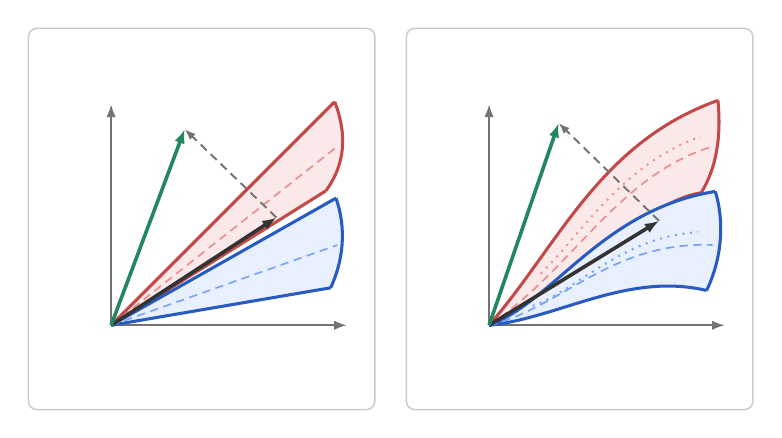
\begin{tikzpicture}
    \ifdefined\ONLYB
        \panelB
    \else
        \ifdefined\ONLYC
            \panelC
        \else
            \panelB
            \begin{scope}[xshift=4.80cm]
                \panelC
            \end{scope}
        \fi
    \fi
\end{tikzpicture}
\end{document}
'
%    xelatex -jobname=fig1_bc_clean '% ---------------------------------------------------------------------------
%  Figure 1 panels (b) and (c) -- TEXT-FREE export for PowerPoint.
%
%  Every label / annotation has been removed (panel titles, axis labels,
%  "$v_t^{cand}$", "$R_{1,\eta}$", "$VO^T_1$", origin "0", correction symbols,
%  the union equations ...).  Geometry, colours and line weights are identical
%  to the in-paper TikZ figure, so text can be re-added by hand in PPT.
%
%  Build from this folder:
%    xelatex -jobname=fig1_b_clean  '\def\ONLYB{}\input{fig1_bc_clean.tex}'
%    xelatex -jobname=fig1_c_clean  '\def\ONLYC{}\input{fig1_bc_clean.tex}'
%    xelatex -jobname=fig1_bc_clean '\input{fig1_bc_clean.tex}'
% ---------------------------------------------------------------------------
\documentclass[tikz,border=2pt]{standalone}

\usepackage{tikz}
\usetikzlibrary{arrows.meta,positioning,calc}

\definecolor{pvoBlue}{HTML}{2F6FED}
\definecolor{pvoGreen}{HTML}{2AA876}
\definecolor{pvoRed}{HTML}{E05252}

\tikzset{
    line join=round, line cap=round,
    panel/.style={rounded corners=3pt, draw=black!20, line width=0.55pt},
    axis/.style={-{Latex[length=1.6mm]}, line width=0.7pt, draw=black!55},
    riskone/.style={line width=1.1pt, draw=pvoRed!88!black},
    risktwo/.style={line width=1.1pt, draw=pvoBlue!82!black},
    meanline/.style={line width=0.62pt, densely dashed},
    candidate/.style={-{Latex[length=1.8mm]}, line width=1.3pt, draw=black!80},
    accepted/.style={-{Latex[length=1.8mm]}, line width=1.3pt, draw=pvoGreen!80!black},
    correction/.style={-{Latex[length=1.4mm]}, line width=0.7pt, densely dashed, draw=black!55}
}

% --------------------------------------------------------------- panel (b) --
\newcommand{\panelB}{%
    \draw[panel] (-0.10,-0.12) rectangle (4.30,4.72);
    \begin{scope}[shift={(0.95,0.95)}, scale=0.85, shift={(-0.48,-0.52)}]
        \draw[axis] (0.48,0.52) -- (4.00,0.52);
        \draw[axis] (0.48,0.52) -- (0.48,3.82);

        % deterministic relative-velocity cone for obstacle 1
        \path[fill=pvoRed!13]
            (0.48,0.52) -- (3.82,3.86)
            .. controls (4.01,3.37) and (3.98,2.93) .. (3.69,2.53) -- cycle;
        \draw[riskone] (0.48,0.52) -- (3.82,3.86);
        \draw[riskone] (0.48,0.52) -- (3.69,2.53);
        \draw[riskone] (3.82,3.86) .. controls (4.01,3.37) and (3.98,2.93) .. (3.69,2.53);
        \draw[meanline, pvoRed!64] (0.48,0.52) -- (3.82,3.16);

        % deterministic relative-velocity cone for obstacle 2
        \path[fill=pvoBlue!11]
            (0.48,0.52) -- (3.84,2.42)
            .. controls (4.00,1.96) and (3.95,1.49) .. (3.76,1.08) -- cycle;
        \draw[risktwo] (0.48,0.52) -- (3.84,2.42);
        \draw[risktwo] (0.48,0.52) -- (3.76,1.08);
        \draw[risktwo] (3.84,2.42) .. controls (4.00,1.96) and (3.95,1.49) .. (3.76,1.08);
        \draw[meanline, pvoBlue!62] (0.48,0.52) -- (3.86,1.72);

        % candidate velocity / filtered velocity / correction
        \draw[candidate] (0.48,0.52) -- (2.95,2.13);
        \draw[accepted] (0.48,0.52) -- (1.58,3.45);
        \draw[correction] (2.95,2.13) -- (1.58,3.45);
    \end{scope}%
}

% --------------------------------------------------------------- panel (c) --
\newcommand{\panelC}{%
    \draw[panel] (-0.10,-0.12) rectangle (4.30,4.72);
    \begin{scope}[shift={(0.95,0.95)}, scale=0.85, shift={(-0.48,-0.52)}]
        \draw[axis] (0.48,0.52) -- (4.00,0.52);
        \draw[axis] (0.48,0.52) -- (0.48,3.82);

        % action-conditioned risk tube for obstacle 1
        \path[fill=pvoRed!13]
            (0.48,0.52)
            .. controls (1.52,1.72) and (2.13,3.25) .. (3.90,3.88)
            .. controls (3.95,3.33) and (3.88,2.88) .. (3.65,2.50)
            .. controls (2.72,2.35) and (1.64,1.02) .. (0.48,0.52) -- cycle;
        \draw[riskone]
            (0.48,0.52) .. controls (1.52,1.72) and (2.13,3.25) .. (3.90,3.88);
        \draw[riskone]
            (0.48,0.52) .. controls (1.64,1.02) and (2.72,2.35) .. (3.65,2.50);
        \draw[riskone] (3.90,3.88) .. controls (3.95,3.33) and (3.88,2.88) .. (3.65,2.50);
        \draw[meanline, pvoRed!65]
            (0.48,0.52) .. controls (1.72,1.35) and (2.38,2.73) .. (3.78,3.18);
        \draw[dotted, line width=0.75pt, pvoRed!62]
            (1.25,1.29) .. controls (1.86,1.88) and (2.46,2.92) .. (3.64,3.34);

        % action-conditioned risk tube for obstacle 2
        \path[fill=pvoBlue!11]
            (0.48,0.52)
            .. controls (1.45,0.88) and (2.17,2.25) .. (3.86,2.52)
            .. controls (4.00,2.06) and (3.96,1.52) .. (3.73,1.04)
            .. controls (2.55,1.32) and (1.53,0.63) .. (0.48,0.52) -- cycle;
        \draw[risktwo]
            (0.48,0.52) .. controls (1.45,0.88) and (2.17,2.25) .. (3.86,2.52);
        \draw[risktwo]
            (0.48,0.52) .. controls (1.53,0.63) and (2.55,1.32) .. (3.73,1.04);
        \draw[risktwo] (3.86,2.52) .. controls (4.00,2.06) and (3.96,1.52) .. (3.73,1.04);
        \draw[meanline, pvoBlue!64]
            (0.48,0.52) .. controls (1.55,0.77) and (2.30,1.78) .. (3.82,1.72);
        \draw[dotted, line width=0.75pt, pvoBlue!62]
            (1.13,0.81) .. controls (1.79,1.04) and (2.48,1.85) .. (3.60,1.91);

        % candidate velocity / filtered velocity / correction
        \draw[candidate] (0.48,0.52) -- (3.02,2.08);
        \draw[accepted] (0.48,0.52) -- (1.52,3.54);
        \draw[correction] (3.02,2.08) -- (1.52,3.54);
    \end{scope}%
}

\begin{document}
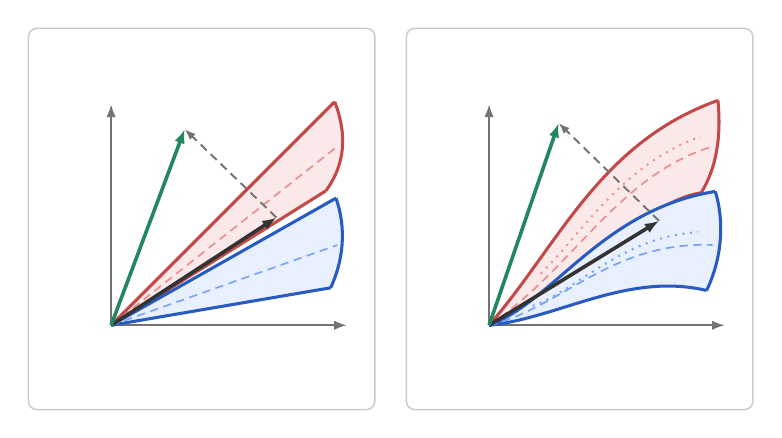
\begin{tikzpicture}
    \ifdefined\ONLYB
        \panelB
    \else
        \ifdefined\ONLYC
            \panelC
        \else
            \panelB
            \begin{scope}[xshift=4.80cm]
                \panelC
            \end{scope}
        \fi
    \fi
\end{tikzpicture}
\end{document}
'
% ---------------------------------------------------------------------------
\documentclass[tikz,border=2pt]{standalone}

\usepackage{tikz}
\usetikzlibrary{arrows.meta,positioning,calc}

\definecolor{pvoBlue}{HTML}{2F6FED}
\definecolor{pvoGreen}{HTML}{2AA876}
\definecolor{pvoRed}{HTML}{E05252}

\tikzset{
    line join=round, line cap=round,
    panel/.style={rounded corners=3pt, draw=black!20, line width=0.55pt},
    axis/.style={-{Latex[length=1.6mm]}, line width=0.7pt, draw=black!55},
    riskone/.style={line width=1.1pt, draw=pvoRed!88!black},
    risktwo/.style={line width=1.1pt, draw=pvoBlue!82!black},
    meanline/.style={line width=0.62pt, densely dashed},
    candidate/.style={-{Latex[length=1.8mm]}, line width=1.3pt, draw=black!80},
    accepted/.style={-{Latex[length=1.8mm]}, line width=1.3pt, draw=pvoGreen!80!black},
    correction/.style={-{Latex[length=1.4mm]}, line width=0.7pt, densely dashed, draw=black!55}
}

% --------------------------------------------------------------- panel (b) --
\newcommand{\panelB}{%
    \draw[panel] (-0.10,-0.12) rectangle (4.30,4.72);
    \begin{scope}[shift={(0.95,0.95)}, scale=0.85, shift={(-0.48,-0.52)}]
        \draw[axis] (0.48,0.52) -- (4.00,0.52);
        \draw[axis] (0.48,0.52) -- (0.48,3.82);

        % deterministic relative-velocity cone for obstacle 1
        \path[fill=pvoRed!13]
            (0.48,0.52) -- (3.82,3.86)
            .. controls (4.01,3.37) and (3.98,2.93) .. (3.69,2.53) -- cycle;
        \draw[riskone] (0.48,0.52) -- (3.82,3.86);
        \draw[riskone] (0.48,0.52) -- (3.69,2.53);
        \draw[riskone] (3.82,3.86) .. controls (4.01,3.37) and (3.98,2.93) .. (3.69,2.53);
        \draw[meanline, pvoRed!64] (0.48,0.52) -- (3.82,3.16);

        % deterministic relative-velocity cone for obstacle 2
        \path[fill=pvoBlue!11]
            (0.48,0.52) -- (3.84,2.42)
            .. controls (4.00,1.96) and (3.95,1.49) .. (3.76,1.08) -- cycle;
        \draw[risktwo] (0.48,0.52) -- (3.84,2.42);
        \draw[risktwo] (0.48,0.52) -- (3.76,1.08);
        \draw[risktwo] (3.84,2.42) .. controls (4.00,1.96) and (3.95,1.49) .. (3.76,1.08);
        \draw[meanline, pvoBlue!62] (0.48,0.52) -- (3.86,1.72);

        % candidate velocity / filtered velocity / correction
        \draw[candidate] (0.48,0.52) -- (2.95,2.13);
        \draw[accepted] (0.48,0.52) -- (1.58,3.45);
        \draw[correction] (2.95,2.13) -- (1.58,3.45);
    \end{scope}%
}

% --------------------------------------------------------------- panel (c) --
\newcommand{\panelC}{%
    \draw[panel] (-0.10,-0.12) rectangle (4.30,4.72);
    \begin{scope}[shift={(0.95,0.95)}, scale=0.85, shift={(-0.48,-0.52)}]
        \draw[axis] (0.48,0.52) -- (4.00,0.52);
        \draw[axis] (0.48,0.52) -- (0.48,3.82);

        % action-conditioned risk tube for obstacle 1
        \path[fill=pvoRed!13]
            (0.48,0.52)
            .. controls (1.52,1.72) and (2.13,3.25) .. (3.90,3.88)
            .. controls (3.95,3.33) and (3.88,2.88) .. (3.65,2.50)
            .. controls (2.72,2.35) and (1.64,1.02) .. (0.48,0.52) -- cycle;
        \draw[riskone]
            (0.48,0.52) .. controls (1.52,1.72) and (2.13,3.25) .. (3.90,3.88);
        \draw[riskone]
            (0.48,0.52) .. controls (1.64,1.02) and (2.72,2.35) .. (3.65,2.50);
        \draw[riskone] (3.90,3.88) .. controls (3.95,3.33) and (3.88,2.88) .. (3.65,2.50);
        \draw[meanline, pvoRed!65]
            (0.48,0.52) .. controls (1.72,1.35) and (2.38,2.73) .. (3.78,3.18);
        \draw[dotted, line width=0.75pt, pvoRed!62]
            (1.25,1.29) .. controls (1.86,1.88) and (2.46,2.92) .. (3.64,3.34);

        % action-conditioned risk tube for obstacle 2
        \path[fill=pvoBlue!11]
            (0.48,0.52)
            .. controls (1.45,0.88) and (2.17,2.25) .. (3.86,2.52)
            .. controls (4.00,2.06) and (3.96,1.52) .. (3.73,1.04)
            .. controls (2.55,1.32) and (1.53,0.63) .. (0.48,0.52) -- cycle;
        \draw[risktwo]
            (0.48,0.52) .. controls (1.45,0.88) and (2.17,2.25) .. (3.86,2.52);
        \draw[risktwo]
            (0.48,0.52) .. controls (1.53,0.63) and (2.55,1.32) .. (3.73,1.04);
        \draw[risktwo] (3.86,2.52) .. controls (4.00,2.06) and (3.96,1.52) .. (3.73,1.04);
        \draw[meanline, pvoBlue!64]
            (0.48,0.52) .. controls (1.55,0.77) and (2.30,1.78) .. (3.82,1.72);
        \draw[dotted, line width=0.75pt, pvoBlue!62]
            (1.13,0.81) .. controls (1.79,1.04) and (2.48,1.85) .. (3.60,1.91);

        % candidate velocity / filtered velocity / correction
        \draw[candidate] (0.48,0.52) -- (3.02,2.08);
        \draw[accepted] (0.48,0.52) -- (1.52,3.54);
        \draw[correction] (3.02,2.08) -- (1.52,3.54);
    \end{scope}%
}

\begin{document}
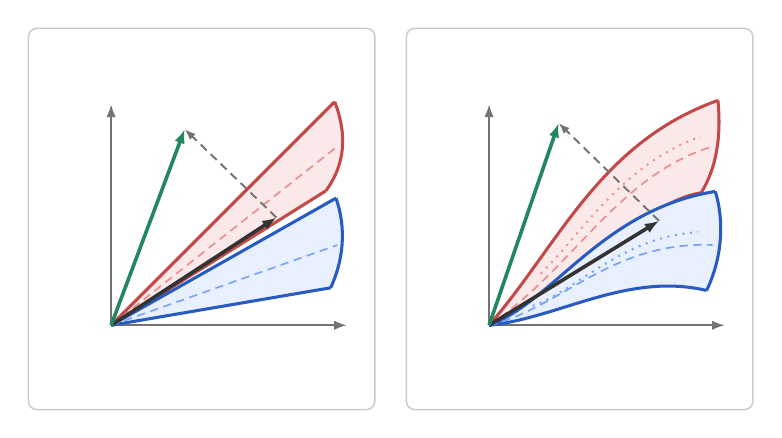
\begin{tikzpicture}
    \ifdefined\ONLYB
        \panelB
    \else
        \ifdefined\ONLYC
            \panelC
        \else
            \panelB
            \begin{scope}[xshift=4.80cm]
                \panelC
            \end{scope}
        \fi
    \fi
\end{tikzpicture}
\end{document}
'
% ---------------------------------------------------------------------------
\documentclass[tikz,border=2pt]{standalone}

\usepackage{tikz}
\usetikzlibrary{arrows.meta,positioning,calc}

\definecolor{pvoBlue}{HTML}{2F6FED}
\definecolor{pvoGreen}{HTML}{2AA876}
\definecolor{pvoRed}{HTML}{E05252}

\tikzset{
    line join=round, line cap=round,
    panel/.style={rounded corners=3pt, draw=black!20, line width=0.55pt},
    axis/.style={-{Latex[length=1.6mm]}, line width=0.7pt, draw=black!55},
    riskone/.style={line width=1.1pt, draw=pvoRed!88!black},
    risktwo/.style={line width=1.1pt, draw=pvoBlue!82!black},
    meanline/.style={line width=0.62pt, densely dashed},
    candidate/.style={-{Latex[length=1.8mm]}, line width=1.3pt, draw=black!80},
    accepted/.style={-{Latex[length=1.8mm]}, line width=1.3pt, draw=pvoGreen!80!black},
    correction/.style={-{Latex[length=1.4mm]}, line width=0.7pt, densely dashed, draw=black!55}
}

% --------------------------------------------------------------- panel (b) --
\newcommand{\panelB}{%
    \draw[panel] (-0.10,-0.12) rectangle (4.30,4.72);
    \begin{scope}[shift={(0.95,0.95)}, scale=0.85, shift={(-0.48,-0.52)}]
        \draw[axis] (0.48,0.52) -- (4.00,0.52);
        \draw[axis] (0.48,0.52) -- (0.48,3.82);

        % deterministic relative-velocity cone for obstacle 1
        \path[fill=pvoRed!13]
            (0.48,0.52) -- (3.82,3.86)
            .. controls (4.01,3.37) and (3.98,2.93) .. (3.69,2.53) -- cycle;
        \draw[riskone] (0.48,0.52) -- (3.82,3.86);
        \draw[riskone] (0.48,0.52) -- (3.69,2.53);
        \draw[riskone] (3.82,3.86) .. controls (4.01,3.37) and (3.98,2.93) .. (3.69,2.53);
        \draw[meanline, pvoRed!64] (0.48,0.52) -- (3.82,3.16);

        % deterministic relative-velocity cone for obstacle 2
        \path[fill=pvoBlue!11]
            (0.48,0.52) -- (3.84,2.42)
            .. controls (4.00,1.96) and (3.95,1.49) .. (3.76,1.08) -- cycle;
        \draw[risktwo] (0.48,0.52) -- (3.84,2.42);
        \draw[risktwo] (0.48,0.52) -- (3.76,1.08);
        \draw[risktwo] (3.84,2.42) .. controls (4.00,1.96) and (3.95,1.49) .. (3.76,1.08);
        \draw[meanline, pvoBlue!62] (0.48,0.52) -- (3.86,1.72);

        % candidate velocity / filtered velocity / correction
        \draw[candidate] (0.48,0.52) -- (2.95,2.13);
        \draw[accepted] (0.48,0.52) -- (1.58,3.45);
        \draw[correction] (2.95,2.13) -- (1.58,3.45);
    \end{scope}%
}

% --------------------------------------------------------------- panel (c) --
\newcommand{\panelC}{%
    \draw[panel] (-0.10,-0.12) rectangle (4.30,4.72);
    \begin{scope}[shift={(0.95,0.95)}, scale=0.85, shift={(-0.48,-0.52)}]
        \draw[axis] (0.48,0.52) -- (4.00,0.52);
        \draw[axis] (0.48,0.52) -- (0.48,3.82);

        % action-conditioned risk tube for obstacle 1
        \path[fill=pvoRed!13]
            (0.48,0.52)
            .. controls (1.52,1.72) and (2.13,3.25) .. (3.90,3.88)
            .. controls (3.95,3.33) and (3.88,2.88) .. (3.65,2.50)
            .. controls (2.72,2.35) and (1.64,1.02) .. (0.48,0.52) -- cycle;
        \draw[riskone]
            (0.48,0.52) .. controls (1.52,1.72) and (2.13,3.25) .. (3.90,3.88);
        \draw[riskone]
            (0.48,0.52) .. controls (1.64,1.02) and (2.72,2.35) .. (3.65,2.50);
        \draw[riskone] (3.90,3.88) .. controls (3.95,3.33) and (3.88,2.88) .. (3.65,2.50);
        \draw[meanline, pvoRed!65]
            (0.48,0.52) .. controls (1.72,1.35) and (2.38,2.73) .. (3.78,3.18);
        \draw[dotted, line width=0.75pt, pvoRed!62]
            (1.25,1.29) .. controls (1.86,1.88) and (2.46,2.92) .. (3.64,3.34);

        % action-conditioned risk tube for obstacle 2
        \path[fill=pvoBlue!11]
            (0.48,0.52)
            .. controls (1.45,0.88) and (2.17,2.25) .. (3.86,2.52)
            .. controls (4.00,2.06) and (3.96,1.52) .. (3.73,1.04)
            .. controls (2.55,1.32) and (1.53,0.63) .. (0.48,0.52) -- cycle;
        \draw[risktwo]
            (0.48,0.52) .. controls (1.45,0.88) and (2.17,2.25) .. (3.86,2.52);
        \draw[risktwo]
            (0.48,0.52) .. controls (1.53,0.63) and (2.55,1.32) .. (3.73,1.04);
        \draw[risktwo] (3.86,2.52) .. controls (4.00,2.06) and (3.96,1.52) .. (3.73,1.04);
        \draw[meanline, pvoBlue!64]
            (0.48,0.52) .. controls (1.55,0.77) and (2.30,1.78) .. (3.82,1.72);
        \draw[dotted, line width=0.75pt, pvoBlue!62]
            (1.13,0.81) .. controls (1.79,1.04) and (2.48,1.85) .. (3.60,1.91);

        % candidate velocity / filtered velocity / correction
        \draw[candidate] (0.48,0.52) -- (3.02,2.08);
        \draw[accepted] (0.48,0.52) -- (1.52,3.54);
        \draw[correction] (3.02,2.08) -- (1.52,3.54);
    \end{scope}%
}

\begin{document}
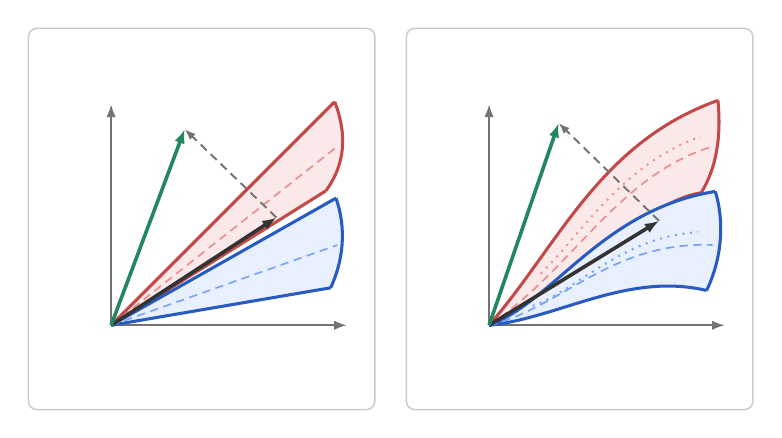
\begin{tikzpicture}
    \ifdefined\ONLYB
        \panelB
    \else
        \ifdefined\ONLYC
            \panelC
        \else
            \panelB
            \begin{scope}[xshift=4.80cm]
                \panelC
            \end{scope}
        \fi
    \fi
\end{tikzpicture}
\end{document}
'
%    xelatex -jobname=fig1_c_clean  '\def\ONLYC{}% ---------------------------------------------------------------------------
%  Figure 1 panels (b) and (c) -- TEXT-FREE export for PowerPoint.
%
%  Every label / annotation has been removed (panel titles, axis labels,
%  "$v_t^{cand}$", "$R_{1,\eta}$", "$VO^T_1$", origin "0", correction symbols,
%  the union equations ...).  Geometry, colours and line weights are identical
%  to the in-paper TikZ figure, so text can be re-added by hand in PPT.
%
%  Build from this folder:
%    xelatex -jobname=fig1_b_clean  '\def\ONLYB{}% ---------------------------------------------------------------------------
%  Figure 1 panels (b) and (c) -- TEXT-FREE export for PowerPoint.
%
%  Every label / annotation has been removed (panel titles, axis labels,
%  "$v_t^{cand}$", "$R_{1,\eta}$", "$VO^T_1$", origin "0", correction symbols,
%  the union equations ...).  Geometry, colours and line weights are identical
%  to the in-paper TikZ figure, so text can be re-added by hand in PPT.
%
%  Build from this folder:
%    xelatex -jobname=fig1_b_clean  '\def\ONLYB{}% ---------------------------------------------------------------------------
%  Figure 1 panels (b) and (c) -- TEXT-FREE export for PowerPoint.
%
%  Every label / annotation has been removed (panel titles, axis labels,
%  "$v_t^{cand}$", "$R_{1,\eta}$", "$VO^T_1$", origin "0", correction symbols,
%  the union equations ...).  Geometry, colours and line weights are identical
%  to the in-paper TikZ figure, so text can be re-added by hand in PPT.
%
%  Build from this folder:
%    xelatex -jobname=fig1_b_clean  '\def\ONLYB{}\input{fig1_bc_clean.tex}'
%    xelatex -jobname=fig1_c_clean  '\def\ONLYC{}\input{fig1_bc_clean.tex}'
%    xelatex -jobname=fig1_bc_clean '\input{fig1_bc_clean.tex}'
% ---------------------------------------------------------------------------
\documentclass[tikz,border=2pt]{standalone}

\usepackage{tikz}
\usetikzlibrary{arrows.meta,positioning,calc}

\definecolor{pvoBlue}{HTML}{2F6FED}
\definecolor{pvoGreen}{HTML}{2AA876}
\definecolor{pvoRed}{HTML}{E05252}

\tikzset{
    line join=round, line cap=round,
    panel/.style={rounded corners=3pt, draw=black!20, line width=0.55pt},
    axis/.style={-{Latex[length=1.6mm]}, line width=0.7pt, draw=black!55},
    riskone/.style={line width=1.1pt, draw=pvoRed!88!black},
    risktwo/.style={line width=1.1pt, draw=pvoBlue!82!black},
    meanline/.style={line width=0.62pt, densely dashed},
    candidate/.style={-{Latex[length=1.8mm]}, line width=1.3pt, draw=black!80},
    accepted/.style={-{Latex[length=1.8mm]}, line width=1.3pt, draw=pvoGreen!80!black},
    correction/.style={-{Latex[length=1.4mm]}, line width=0.7pt, densely dashed, draw=black!55}
}

% --------------------------------------------------------------- panel (b) --
\newcommand{\panelB}{%
    \draw[panel] (-0.10,-0.12) rectangle (4.30,4.72);
    \begin{scope}[shift={(0.95,0.95)}, scale=0.85, shift={(-0.48,-0.52)}]
        \draw[axis] (0.48,0.52) -- (4.00,0.52);
        \draw[axis] (0.48,0.52) -- (0.48,3.82);

        % deterministic relative-velocity cone for obstacle 1
        \path[fill=pvoRed!13]
            (0.48,0.52) -- (3.82,3.86)
            .. controls (4.01,3.37) and (3.98,2.93) .. (3.69,2.53) -- cycle;
        \draw[riskone] (0.48,0.52) -- (3.82,3.86);
        \draw[riskone] (0.48,0.52) -- (3.69,2.53);
        \draw[riskone] (3.82,3.86) .. controls (4.01,3.37) and (3.98,2.93) .. (3.69,2.53);
        \draw[meanline, pvoRed!64] (0.48,0.52) -- (3.82,3.16);

        % deterministic relative-velocity cone for obstacle 2
        \path[fill=pvoBlue!11]
            (0.48,0.52) -- (3.84,2.42)
            .. controls (4.00,1.96) and (3.95,1.49) .. (3.76,1.08) -- cycle;
        \draw[risktwo] (0.48,0.52) -- (3.84,2.42);
        \draw[risktwo] (0.48,0.52) -- (3.76,1.08);
        \draw[risktwo] (3.84,2.42) .. controls (4.00,1.96) and (3.95,1.49) .. (3.76,1.08);
        \draw[meanline, pvoBlue!62] (0.48,0.52) -- (3.86,1.72);

        % candidate velocity / filtered velocity / correction
        \draw[candidate] (0.48,0.52) -- (2.95,2.13);
        \draw[accepted] (0.48,0.52) -- (1.58,3.45);
        \draw[correction] (2.95,2.13) -- (1.58,3.45);
    \end{scope}%
}

% --------------------------------------------------------------- panel (c) --
\newcommand{\panelC}{%
    \draw[panel] (-0.10,-0.12) rectangle (4.30,4.72);
    \begin{scope}[shift={(0.95,0.95)}, scale=0.85, shift={(-0.48,-0.52)}]
        \draw[axis] (0.48,0.52) -- (4.00,0.52);
        \draw[axis] (0.48,0.52) -- (0.48,3.82);

        % action-conditioned risk tube for obstacle 1
        \path[fill=pvoRed!13]
            (0.48,0.52)
            .. controls (1.52,1.72) and (2.13,3.25) .. (3.90,3.88)
            .. controls (3.95,3.33) and (3.88,2.88) .. (3.65,2.50)
            .. controls (2.72,2.35) and (1.64,1.02) .. (0.48,0.52) -- cycle;
        \draw[riskone]
            (0.48,0.52) .. controls (1.52,1.72) and (2.13,3.25) .. (3.90,3.88);
        \draw[riskone]
            (0.48,0.52) .. controls (1.64,1.02) and (2.72,2.35) .. (3.65,2.50);
        \draw[riskone] (3.90,3.88) .. controls (3.95,3.33) and (3.88,2.88) .. (3.65,2.50);
        \draw[meanline, pvoRed!65]
            (0.48,0.52) .. controls (1.72,1.35) and (2.38,2.73) .. (3.78,3.18);
        \draw[dotted, line width=0.75pt, pvoRed!62]
            (1.25,1.29) .. controls (1.86,1.88) and (2.46,2.92) .. (3.64,3.34);

        % action-conditioned risk tube for obstacle 2
        \path[fill=pvoBlue!11]
            (0.48,0.52)
            .. controls (1.45,0.88) and (2.17,2.25) .. (3.86,2.52)
            .. controls (4.00,2.06) and (3.96,1.52) .. (3.73,1.04)
            .. controls (2.55,1.32) and (1.53,0.63) .. (0.48,0.52) -- cycle;
        \draw[risktwo]
            (0.48,0.52) .. controls (1.45,0.88) and (2.17,2.25) .. (3.86,2.52);
        \draw[risktwo]
            (0.48,0.52) .. controls (1.53,0.63) and (2.55,1.32) .. (3.73,1.04);
        \draw[risktwo] (3.86,2.52) .. controls (4.00,2.06) and (3.96,1.52) .. (3.73,1.04);
        \draw[meanline, pvoBlue!64]
            (0.48,0.52) .. controls (1.55,0.77) and (2.30,1.78) .. (3.82,1.72);
        \draw[dotted, line width=0.75pt, pvoBlue!62]
            (1.13,0.81) .. controls (1.79,1.04) and (2.48,1.85) .. (3.60,1.91);

        % candidate velocity / filtered velocity / correction
        \draw[candidate] (0.48,0.52) -- (3.02,2.08);
        \draw[accepted] (0.48,0.52) -- (1.52,3.54);
        \draw[correction] (3.02,2.08) -- (1.52,3.54);
    \end{scope}%
}

\begin{document}
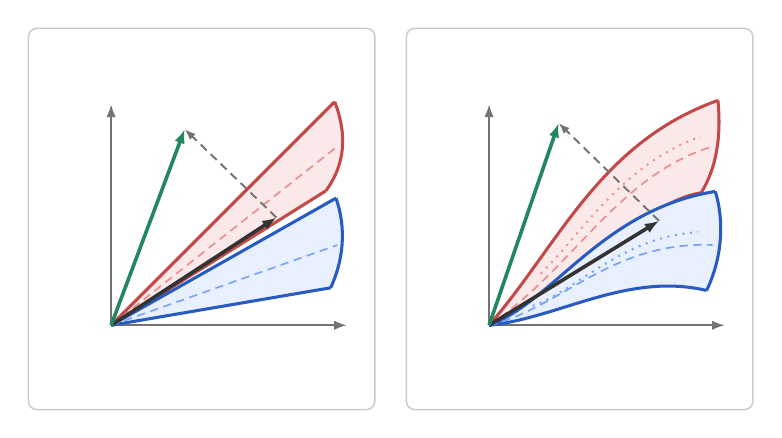
\begin{tikzpicture}
    \ifdefined\ONLYB
        \panelB
    \else
        \ifdefined\ONLYC
            \panelC
        \else
            \panelB
            \begin{scope}[xshift=4.80cm]
                \panelC
            \end{scope}
        \fi
    \fi
\end{tikzpicture}
\end{document}
'
%    xelatex -jobname=fig1_c_clean  '\def\ONLYC{}% ---------------------------------------------------------------------------
%  Figure 1 panels (b) and (c) -- TEXT-FREE export for PowerPoint.
%
%  Every label / annotation has been removed (panel titles, axis labels,
%  "$v_t^{cand}$", "$R_{1,\eta}$", "$VO^T_1$", origin "0", correction symbols,
%  the union equations ...).  Geometry, colours and line weights are identical
%  to the in-paper TikZ figure, so text can be re-added by hand in PPT.
%
%  Build from this folder:
%    xelatex -jobname=fig1_b_clean  '\def\ONLYB{}\input{fig1_bc_clean.tex}'
%    xelatex -jobname=fig1_c_clean  '\def\ONLYC{}\input{fig1_bc_clean.tex}'
%    xelatex -jobname=fig1_bc_clean '\input{fig1_bc_clean.tex}'
% ---------------------------------------------------------------------------
\documentclass[tikz,border=2pt]{standalone}

\usepackage{tikz}
\usetikzlibrary{arrows.meta,positioning,calc}

\definecolor{pvoBlue}{HTML}{2F6FED}
\definecolor{pvoGreen}{HTML}{2AA876}
\definecolor{pvoRed}{HTML}{E05252}

\tikzset{
    line join=round, line cap=round,
    panel/.style={rounded corners=3pt, draw=black!20, line width=0.55pt},
    axis/.style={-{Latex[length=1.6mm]}, line width=0.7pt, draw=black!55},
    riskone/.style={line width=1.1pt, draw=pvoRed!88!black},
    risktwo/.style={line width=1.1pt, draw=pvoBlue!82!black},
    meanline/.style={line width=0.62pt, densely dashed},
    candidate/.style={-{Latex[length=1.8mm]}, line width=1.3pt, draw=black!80},
    accepted/.style={-{Latex[length=1.8mm]}, line width=1.3pt, draw=pvoGreen!80!black},
    correction/.style={-{Latex[length=1.4mm]}, line width=0.7pt, densely dashed, draw=black!55}
}

% --------------------------------------------------------------- panel (b) --
\newcommand{\panelB}{%
    \draw[panel] (-0.10,-0.12) rectangle (4.30,4.72);
    \begin{scope}[shift={(0.95,0.95)}, scale=0.85, shift={(-0.48,-0.52)}]
        \draw[axis] (0.48,0.52) -- (4.00,0.52);
        \draw[axis] (0.48,0.52) -- (0.48,3.82);

        % deterministic relative-velocity cone for obstacle 1
        \path[fill=pvoRed!13]
            (0.48,0.52) -- (3.82,3.86)
            .. controls (4.01,3.37) and (3.98,2.93) .. (3.69,2.53) -- cycle;
        \draw[riskone] (0.48,0.52) -- (3.82,3.86);
        \draw[riskone] (0.48,0.52) -- (3.69,2.53);
        \draw[riskone] (3.82,3.86) .. controls (4.01,3.37) and (3.98,2.93) .. (3.69,2.53);
        \draw[meanline, pvoRed!64] (0.48,0.52) -- (3.82,3.16);

        % deterministic relative-velocity cone for obstacle 2
        \path[fill=pvoBlue!11]
            (0.48,0.52) -- (3.84,2.42)
            .. controls (4.00,1.96) and (3.95,1.49) .. (3.76,1.08) -- cycle;
        \draw[risktwo] (0.48,0.52) -- (3.84,2.42);
        \draw[risktwo] (0.48,0.52) -- (3.76,1.08);
        \draw[risktwo] (3.84,2.42) .. controls (4.00,1.96) and (3.95,1.49) .. (3.76,1.08);
        \draw[meanline, pvoBlue!62] (0.48,0.52) -- (3.86,1.72);

        % candidate velocity / filtered velocity / correction
        \draw[candidate] (0.48,0.52) -- (2.95,2.13);
        \draw[accepted] (0.48,0.52) -- (1.58,3.45);
        \draw[correction] (2.95,2.13) -- (1.58,3.45);
    \end{scope}%
}

% --------------------------------------------------------------- panel (c) --
\newcommand{\panelC}{%
    \draw[panel] (-0.10,-0.12) rectangle (4.30,4.72);
    \begin{scope}[shift={(0.95,0.95)}, scale=0.85, shift={(-0.48,-0.52)}]
        \draw[axis] (0.48,0.52) -- (4.00,0.52);
        \draw[axis] (0.48,0.52) -- (0.48,3.82);

        % action-conditioned risk tube for obstacle 1
        \path[fill=pvoRed!13]
            (0.48,0.52)
            .. controls (1.52,1.72) and (2.13,3.25) .. (3.90,3.88)
            .. controls (3.95,3.33) and (3.88,2.88) .. (3.65,2.50)
            .. controls (2.72,2.35) and (1.64,1.02) .. (0.48,0.52) -- cycle;
        \draw[riskone]
            (0.48,0.52) .. controls (1.52,1.72) and (2.13,3.25) .. (3.90,3.88);
        \draw[riskone]
            (0.48,0.52) .. controls (1.64,1.02) and (2.72,2.35) .. (3.65,2.50);
        \draw[riskone] (3.90,3.88) .. controls (3.95,3.33) and (3.88,2.88) .. (3.65,2.50);
        \draw[meanline, pvoRed!65]
            (0.48,0.52) .. controls (1.72,1.35) and (2.38,2.73) .. (3.78,3.18);
        \draw[dotted, line width=0.75pt, pvoRed!62]
            (1.25,1.29) .. controls (1.86,1.88) and (2.46,2.92) .. (3.64,3.34);

        % action-conditioned risk tube for obstacle 2
        \path[fill=pvoBlue!11]
            (0.48,0.52)
            .. controls (1.45,0.88) and (2.17,2.25) .. (3.86,2.52)
            .. controls (4.00,2.06) and (3.96,1.52) .. (3.73,1.04)
            .. controls (2.55,1.32) and (1.53,0.63) .. (0.48,0.52) -- cycle;
        \draw[risktwo]
            (0.48,0.52) .. controls (1.45,0.88) and (2.17,2.25) .. (3.86,2.52);
        \draw[risktwo]
            (0.48,0.52) .. controls (1.53,0.63) and (2.55,1.32) .. (3.73,1.04);
        \draw[risktwo] (3.86,2.52) .. controls (4.00,2.06) and (3.96,1.52) .. (3.73,1.04);
        \draw[meanline, pvoBlue!64]
            (0.48,0.52) .. controls (1.55,0.77) and (2.30,1.78) .. (3.82,1.72);
        \draw[dotted, line width=0.75pt, pvoBlue!62]
            (1.13,0.81) .. controls (1.79,1.04) and (2.48,1.85) .. (3.60,1.91);

        % candidate velocity / filtered velocity / correction
        \draw[candidate] (0.48,0.52) -- (3.02,2.08);
        \draw[accepted] (0.48,0.52) -- (1.52,3.54);
        \draw[correction] (3.02,2.08) -- (1.52,3.54);
    \end{scope}%
}

\begin{document}
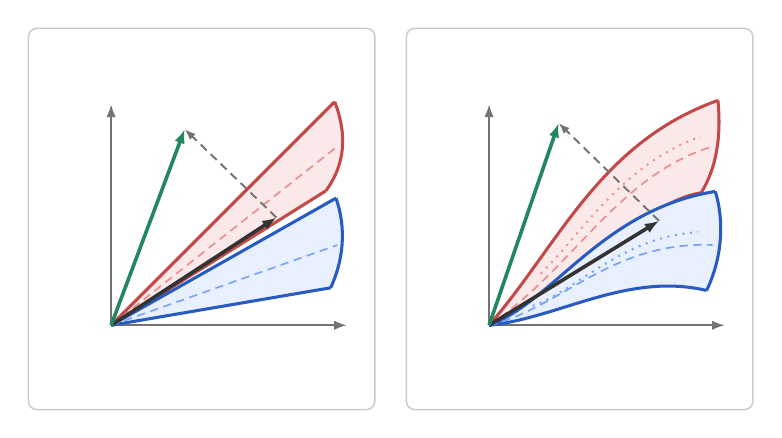
\begin{tikzpicture}
    \ifdefined\ONLYB
        \panelB
    \else
        \ifdefined\ONLYC
            \panelC
        \else
            \panelB
            \begin{scope}[xshift=4.80cm]
                \panelC
            \end{scope}
        \fi
    \fi
\end{tikzpicture}
\end{document}
'
%    xelatex -jobname=fig1_bc_clean '% ---------------------------------------------------------------------------
%  Figure 1 panels (b) and (c) -- TEXT-FREE export for PowerPoint.
%
%  Every label / annotation has been removed (panel titles, axis labels,
%  "$v_t^{cand}$", "$R_{1,\eta}$", "$VO^T_1$", origin "0", correction symbols,
%  the union equations ...).  Geometry, colours and line weights are identical
%  to the in-paper TikZ figure, so text can be re-added by hand in PPT.
%
%  Build from this folder:
%    xelatex -jobname=fig1_b_clean  '\def\ONLYB{}\input{fig1_bc_clean.tex}'
%    xelatex -jobname=fig1_c_clean  '\def\ONLYC{}\input{fig1_bc_clean.tex}'
%    xelatex -jobname=fig1_bc_clean '\input{fig1_bc_clean.tex}'
% ---------------------------------------------------------------------------
\documentclass[tikz,border=2pt]{standalone}

\usepackage{tikz}
\usetikzlibrary{arrows.meta,positioning,calc}

\definecolor{pvoBlue}{HTML}{2F6FED}
\definecolor{pvoGreen}{HTML}{2AA876}
\definecolor{pvoRed}{HTML}{E05252}

\tikzset{
    line join=round, line cap=round,
    panel/.style={rounded corners=3pt, draw=black!20, line width=0.55pt},
    axis/.style={-{Latex[length=1.6mm]}, line width=0.7pt, draw=black!55},
    riskone/.style={line width=1.1pt, draw=pvoRed!88!black},
    risktwo/.style={line width=1.1pt, draw=pvoBlue!82!black},
    meanline/.style={line width=0.62pt, densely dashed},
    candidate/.style={-{Latex[length=1.8mm]}, line width=1.3pt, draw=black!80},
    accepted/.style={-{Latex[length=1.8mm]}, line width=1.3pt, draw=pvoGreen!80!black},
    correction/.style={-{Latex[length=1.4mm]}, line width=0.7pt, densely dashed, draw=black!55}
}

% --------------------------------------------------------------- panel (b) --
\newcommand{\panelB}{%
    \draw[panel] (-0.10,-0.12) rectangle (4.30,4.72);
    \begin{scope}[shift={(0.95,0.95)}, scale=0.85, shift={(-0.48,-0.52)}]
        \draw[axis] (0.48,0.52) -- (4.00,0.52);
        \draw[axis] (0.48,0.52) -- (0.48,3.82);

        % deterministic relative-velocity cone for obstacle 1
        \path[fill=pvoRed!13]
            (0.48,0.52) -- (3.82,3.86)
            .. controls (4.01,3.37) and (3.98,2.93) .. (3.69,2.53) -- cycle;
        \draw[riskone] (0.48,0.52) -- (3.82,3.86);
        \draw[riskone] (0.48,0.52) -- (3.69,2.53);
        \draw[riskone] (3.82,3.86) .. controls (4.01,3.37) and (3.98,2.93) .. (3.69,2.53);
        \draw[meanline, pvoRed!64] (0.48,0.52) -- (3.82,3.16);

        % deterministic relative-velocity cone for obstacle 2
        \path[fill=pvoBlue!11]
            (0.48,0.52) -- (3.84,2.42)
            .. controls (4.00,1.96) and (3.95,1.49) .. (3.76,1.08) -- cycle;
        \draw[risktwo] (0.48,0.52) -- (3.84,2.42);
        \draw[risktwo] (0.48,0.52) -- (3.76,1.08);
        \draw[risktwo] (3.84,2.42) .. controls (4.00,1.96) and (3.95,1.49) .. (3.76,1.08);
        \draw[meanline, pvoBlue!62] (0.48,0.52) -- (3.86,1.72);

        % candidate velocity / filtered velocity / correction
        \draw[candidate] (0.48,0.52) -- (2.95,2.13);
        \draw[accepted] (0.48,0.52) -- (1.58,3.45);
        \draw[correction] (2.95,2.13) -- (1.58,3.45);
    \end{scope}%
}

% --------------------------------------------------------------- panel (c) --
\newcommand{\panelC}{%
    \draw[panel] (-0.10,-0.12) rectangle (4.30,4.72);
    \begin{scope}[shift={(0.95,0.95)}, scale=0.85, shift={(-0.48,-0.52)}]
        \draw[axis] (0.48,0.52) -- (4.00,0.52);
        \draw[axis] (0.48,0.52) -- (0.48,3.82);

        % action-conditioned risk tube for obstacle 1
        \path[fill=pvoRed!13]
            (0.48,0.52)
            .. controls (1.52,1.72) and (2.13,3.25) .. (3.90,3.88)
            .. controls (3.95,3.33) and (3.88,2.88) .. (3.65,2.50)
            .. controls (2.72,2.35) and (1.64,1.02) .. (0.48,0.52) -- cycle;
        \draw[riskone]
            (0.48,0.52) .. controls (1.52,1.72) and (2.13,3.25) .. (3.90,3.88);
        \draw[riskone]
            (0.48,0.52) .. controls (1.64,1.02) and (2.72,2.35) .. (3.65,2.50);
        \draw[riskone] (3.90,3.88) .. controls (3.95,3.33) and (3.88,2.88) .. (3.65,2.50);
        \draw[meanline, pvoRed!65]
            (0.48,0.52) .. controls (1.72,1.35) and (2.38,2.73) .. (3.78,3.18);
        \draw[dotted, line width=0.75pt, pvoRed!62]
            (1.25,1.29) .. controls (1.86,1.88) and (2.46,2.92) .. (3.64,3.34);

        % action-conditioned risk tube for obstacle 2
        \path[fill=pvoBlue!11]
            (0.48,0.52)
            .. controls (1.45,0.88) and (2.17,2.25) .. (3.86,2.52)
            .. controls (4.00,2.06) and (3.96,1.52) .. (3.73,1.04)
            .. controls (2.55,1.32) and (1.53,0.63) .. (0.48,0.52) -- cycle;
        \draw[risktwo]
            (0.48,0.52) .. controls (1.45,0.88) and (2.17,2.25) .. (3.86,2.52);
        \draw[risktwo]
            (0.48,0.52) .. controls (1.53,0.63) and (2.55,1.32) .. (3.73,1.04);
        \draw[risktwo] (3.86,2.52) .. controls (4.00,2.06) and (3.96,1.52) .. (3.73,1.04);
        \draw[meanline, pvoBlue!64]
            (0.48,0.52) .. controls (1.55,0.77) and (2.30,1.78) .. (3.82,1.72);
        \draw[dotted, line width=0.75pt, pvoBlue!62]
            (1.13,0.81) .. controls (1.79,1.04) and (2.48,1.85) .. (3.60,1.91);

        % candidate velocity / filtered velocity / correction
        \draw[candidate] (0.48,0.52) -- (3.02,2.08);
        \draw[accepted] (0.48,0.52) -- (1.52,3.54);
        \draw[correction] (3.02,2.08) -- (1.52,3.54);
    \end{scope}%
}

\begin{document}
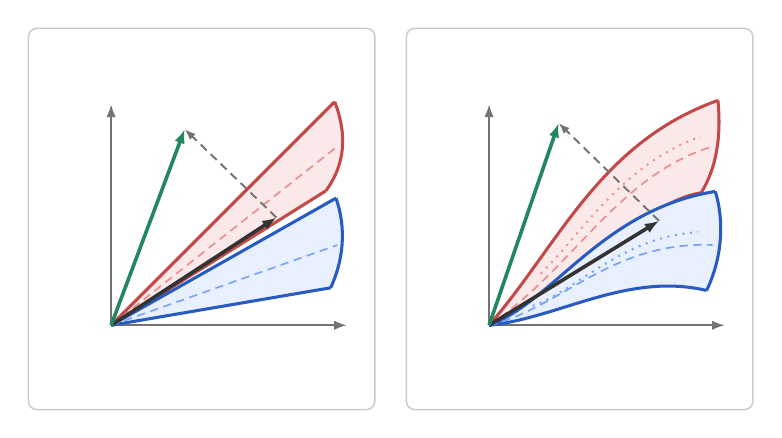
\begin{tikzpicture}
    \ifdefined\ONLYB
        \panelB
    \else
        \ifdefined\ONLYC
            \panelC
        \else
            \panelB
            \begin{scope}[xshift=4.80cm]
                \panelC
            \end{scope}
        \fi
    \fi
\end{tikzpicture}
\end{document}
'
% ---------------------------------------------------------------------------
\documentclass[tikz,border=2pt]{standalone}

\usepackage{tikz}
\usetikzlibrary{arrows.meta,positioning,calc}

\definecolor{pvoBlue}{HTML}{2F6FED}
\definecolor{pvoGreen}{HTML}{2AA876}
\definecolor{pvoRed}{HTML}{E05252}

\tikzset{
    line join=round, line cap=round,
    panel/.style={rounded corners=3pt, draw=black!20, line width=0.55pt},
    axis/.style={-{Latex[length=1.6mm]}, line width=0.7pt, draw=black!55},
    riskone/.style={line width=1.1pt, draw=pvoRed!88!black},
    risktwo/.style={line width=1.1pt, draw=pvoBlue!82!black},
    meanline/.style={line width=0.62pt, densely dashed},
    candidate/.style={-{Latex[length=1.8mm]}, line width=1.3pt, draw=black!80},
    accepted/.style={-{Latex[length=1.8mm]}, line width=1.3pt, draw=pvoGreen!80!black},
    correction/.style={-{Latex[length=1.4mm]}, line width=0.7pt, densely dashed, draw=black!55}
}

% --------------------------------------------------------------- panel (b) --
\newcommand{\panelB}{%
    \draw[panel] (-0.10,-0.12) rectangle (4.30,4.72);
    \begin{scope}[shift={(0.95,0.95)}, scale=0.85, shift={(-0.48,-0.52)}]
        \draw[axis] (0.48,0.52) -- (4.00,0.52);
        \draw[axis] (0.48,0.52) -- (0.48,3.82);

        % deterministic relative-velocity cone for obstacle 1
        \path[fill=pvoRed!13]
            (0.48,0.52) -- (3.82,3.86)
            .. controls (4.01,3.37) and (3.98,2.93) .. (3.69,2.53) -- cycle;
        \draw[riskone] (0.48,0.52) -- (3.82,3.86);
        \draw[riskone] (0.48,0.52) -- (3.69,2.53);
        \draw[riskone] (3.82,3.86) .. controls (4.01,3.37) and (3.98,2.93) .. (3.69,2.53);
        \draw[meanline, pvoRed!64] (0.48,0.52) -- (3.82,3.16);

        % deterministic relative-velocity cone for obstacle 2
        \path[fill=pvoBlue!11]
            (0.48,0.52) -- (3.84,2.42)
            .. controls (4.00,1.96) and (3.95,1.49) .. (3.76,1.08) -- cycle;
        \draw[risktwo] (0.48,0.52) -- (3.84,2.42);
        \draw[risktwo] (0.48,0.52) -- (3.76,1.08);
        \draw[risktwo] (3.84,2.42) .. controls (4.00,1.96) and (3.95,1.49) .. (3.76,1.08);
        \draw[meanline, pvoBlue!62] (0.48,0.52) -- (3.86,1.72);

        % candidate velocity / filtered velocity / correction
        \draw[candidate] (0.48,0.52) -- (2.95,2.13);
        \draw[accepted] (0.48,0.52) -- (1.58,3.45);
        \draw[correction] (2.95,2.13) -- (1.58,3.45);
    \end{scope}%
}

% --------------------------------------------------------------- panel (c) --
\newcommand{\panelC}{%
    \draw[panel] (-0.10,-0.12) rectangle (4.30,4.72);
    \begin{scope}[shift={(0.95,0.95)}, scale=0.85, shift={(-0.48,-0.52)}]
        \draw[axis] (0.48,0.52) -- (4.00,0.52);
        \draw[axis] (0.48,0.52) -- (0.48,3.82);

        % action-conditioned risk tube for obstacle 1
        \path[fill=pvoRed!13]
            (0.48,0.52)
            .. controls (1.52,1.72) and (2.13,3.25) .. (3.90,3.88)
            .. controls (3.95,3.33) and (3.88,2.88) .. (3.65,2.50)
            .. controls (2.72,2.35) and (1.64,1.02) .. (0.48,0.52) -- cycle;
        \draw[riskone]
            (0.48,0.52) .. controls (1.52,1.72) and (2.13,3.25) .. (3.90,3.88);
        \draw[riskone]
            (0.48,0.52) .. controls (1.64,1.02) and (2.72,2.35) .. (3.65,2.50);
        \draw[riskone] (3.90,3.88) .. controls (3.95,3.33) and (3.88,2.88) .. (3.65,2.50);
        \draw[meanline, pvoRed!65]
            (0.48,0.52) .. controls (1.72,1.35) and (2.38,2.73) .. (3.78,3.18);
        \draw[dotted, line width=0.75pt, pvoRed!62]
            (1.25,1.29) .. controls (1.86,1.88) and (2.46,2.92) .. (3.64,3.34);

        % action-conditioned risk tube for obstacle 2
        \path[fill=pvoBlue!11]
            (0.48,0.52)
            .. controls (1.45,0.88) and (2.17,2.25) .. (3.86,2.52)
            .. controls (4.00,2.06) and (3.96,1.52) .. (3.73,1.04)
            .. controls (2.55,1.32) and (1.53,0.63) .. (0.48,0.52) -- cycle;
        \draw[risktwo]
            (0.48,0.52) .. controls (1.45,0.88) and (2.17,2.25) .. (3.86,2.52);
        \draw[risktwo]
            (0.48,0.52) .. controls (1.53,0.63) and (2.55,1.32) .. (3.73,1.04);
        \draw[risktwo] (3.86,2.52) .. controls (4.00,2.06) and (3.96,1.52) .. (3.73,1.04);
        \draw[meanline, pvoBlue!64]
            (0.48,0.52) .. controls (1.55,0.77) and (2.30,1.78) .. (3.82,1.72);
        \draw[dotted, line width=0.75pt, pvoBlue!62]
            (1.13,0.81) .. controls (1.79,1.04) and (2.48,1.85) .. (3.60,1.91);

        % candidate velocity / filtered velocity / correction
        \draw[candidate] (0.48,0.52) -- (3.02,2.08);
        \draw[accepted] (0.48,0.52) -- (1.52,3.54);
        \draw[correction] (3.02,2.08) -- (1.52,3.54);
    \end{scope}%
}

\begin{document}
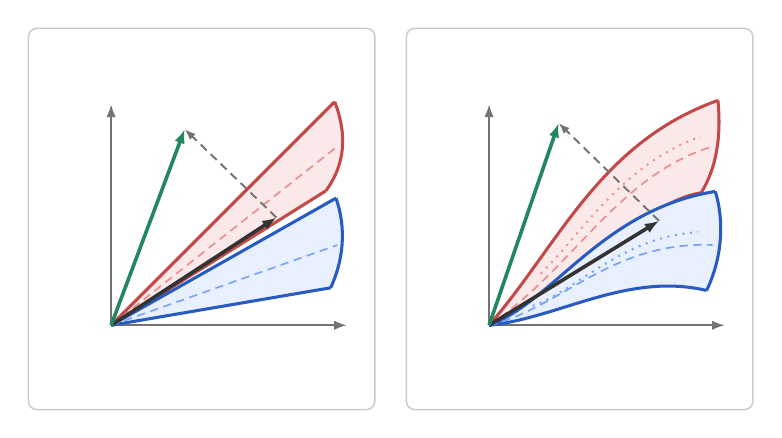
\begin{tikzpicture}
    \ifdefined\ONLYB
        \panelB
    \else
        \ifdefined\ONLYC
            \panelC
        \else
            \panelB
            \begin{scope}[xshift=4.80cm]
                \panelC
            \end{scope}
        \fi
    \fi
\end{tikzpicture}
\end{document}
'
%    xelatex -jobname=fig1_c_clean  '\def\ONLYC{}% ---------------------------------------------------------------------------
%  Figure 1 panels (b) and (c) -- TEXT-FREE export for PowerPoint.
%
%  Every label / annotation has been removed (panel titles, axis labels,
%  "$v_t^{cand}$", "$R_{1,\eta}$", "$VO^T_1$", origin "0", correction symbols,
%  the union equations ...).  Geometry, colours and line weights are identical
%  to the in-paper TikZ figure, so text can be re-added by hand in PPT.
%
%  Build from this folder:
%    xelatex -jobname=fig1_b_clean  '\def\ONLYB{}% ---------------------------------------------------------------------------
%  Figure 1 panels (b) and (c) -- TEXT-FREE export for PowerPoint.
%
%  Every label / annotation has been removed (panel titles, axis labels,
%  "$v_t^{cand}$", "$R_{1,\eta}$", "$VO^T_1$", origin "0", correction symbols,
%  the union equations ...).  Geometry, colours and line weights are identical
%  to the in-paper TikZ figure, so text can be re-added by hand in PPT.
%
%  Build from this folder:
%    xelatex -jobname=fig1_b_clean  '\def\ONLYB{}\input{fig1_bc_clean.tex}'
%    xelatex -jobname=fig1_c_clean  '\def\ONLYC{}\input{fig1_bc_clean.tex}'
%    xelatex -jobname=fig1_bc_clean '\input{fig1_bc_clean.tex}'
% ---------------------------------------------------------------------------
\documentclass[tikz,border=2pt]{standalone}

\usepackage{tikz}
\usetikzlibrary{arrows.meta,positioning,calc}

\definecolor{pvoBlue}{HTML}{2F6FED}
\definecolor{pvoGreen}{HTML}{2AA876}
\definecolor{pvoRed}{HTML}{E05252}

\tikzset{
    line join=round, line cap=round,
    panel/.style={rounded corners=3pt, draw=black!20, line width=0.55pt},
    axis/.style={-{Latex[length=1.6mm]}, line width=0.7pt, draw=black!55},
    riskone/.style={line width=1.1pt, draw=pvoRed!88!black},
    risktwo/.style={line width=1.1pt, draw=pvoBlue!82!black},
    meanline/.style={line width=0.62pt, densely dashed},
    candidate/.style={-{Latex[length=1.8mm]}, line width=1.3pt, draw=black!80},
    accepted/.style={-{Latex[length=1.8mm]}, line width=1.3pt, draw=pvoGreen!80!black},
    correction/.style={-{Latex[length=1.4mm]}, line width=0.7pt, densely dashed, draw=black!55}
}

% --------------------------------------------------------------- panel (b) --
\newcommand{\panelB}{%
    \draw[panel] (-0.10,-0.12) rectangle (4.30,4.72);
    \begin{scope}[shift={(0.95,0.95)}, scale=0.85, shift={(-0.48,-0.52)}]
        \draw[axis] (0.48,0.52) -- (4.00,0.52);
        \draw[axis] (0.48,0.52) -- (0.48,3.82);

        % deterministic relative-velocity cone for obstacle 1
        \path[fill=pvoRed!13]
            (0.48,0.52) -- (3.82,3.86)
            .. controls (4.01,3.37) and (3.98,2.93) .. (3.69,2.53) -- cycle;
        \draw[riskone] (0.48,0.52) -- (3.82,3.86);
        \draw[riskone] (0.48,0.52) -- (3.69,2.53);
        \draw[riskone] (3.82,3.86) .. controls (4.01,3.37) and (3.98,2.93) .. (3.69,2.53);
        \draw[meanline, pvoRed!64] (0.48,0.52) -- (3.82,3.16);

        % deterministic relative-velocity cone for obstacle 2
        \path[fill=pvoBlue!11]
            (0.48,0.52) -- (3.84,2.42)
            .. controls (4.00,1.96) and (3.95,1.49) .. (3.76,1.08) -- cycle;
        \draw[risktwo] (0.48,0.52) -- (3.84,2.42);
        \draw[risktwo] (0.48,0.52) -- (3.76,1.08);
        \draw[risktwo] (3.84,2.42) .. controls (4.00,1.96) and (3.95,1.49) .. (3.76,1.08);
        \draw[meanline, pvoBlue!62] (0.48,0.52) -- (3.86,1.72);

        % candidate velocity / filtered velocity / correction
        \draw[candidate] (0.48,0.52) -- (2.95,2.13);
        \draw[accepted] (0.48,0.52) -- (1.58,3.45);
        \draw[correction] (2.95,2.13) -- (1.58,3.45);
    \end{scope}%
}

% --------------------------------------------------------------- panel (c) --
\newcommand{\panelC}{%
    \draw[panel] (-0.10,-0.12) rectangle (4.30,4.72);
    \begin{scope}[shift={(0.95,0.95)}, scale=0.85, shift={(-0.48,-0.52)}]
        \draw[axis] (0.48,0.52) -- (4.00,0.52);
        \draw[axis] (0.48,0.52) -- (0.48,3.82);

        % action-conditioned risk tube for obstacle 1
        \path[fill=pvoRed!13]
            (0.48,0.52)
            .. controls (1.52,1.72) and (2.13,3.25) .. (3.90,3.88)
            .. controls (3.95,3.33) and (3.88,2.88) .. (3.65,2.50)
            .. controls (2.72,2.35) and (1.64,1.02) .. (0.48,0.52) -- cycle;
        \draw[riskone]
            (0.48,0.52) .. controls (1.52,1.72) and (2.13,3.25) .. (3.90,3.88);
        \draw[riskone]
            (0.48,0.52) .. controls (1.64,1.02) and (2.72,2.35) .. (3.65,2.50);
        \draw[riskone] (3.90,3.88) .. controls (3.95,3.33) and (3.88,2.88) .. (3.65,2.50);
        \draw[meanline, pvoRed!65]
            (0.48,0.52) .. controls (1.72,1.35) and (2.38,2.73) .. (3.78,3.18);
        \draw[dotted, line width=0.75pt, pvoRed!62]
            (1.25,1.29) .. controls (1.86,1.88) and (2.46,2.92) .. (3.64,3.34);

        % action-conditioned risk tube for obstacle 2
        \path[fill=pvoBlue!11]
            (0.48,0.52)
            .. controls (1.45,0.88) and (2.17,2.25) .. (3.86,2.52)
            .. controls (4.00,2.06) and (3.96,1.52) .. (3.73,1.04)
            .. controls (2.55,1.32) and (1.53,0.63) .. (0.48,0.52) -- cycle;
        \draw[risktwo]
            (0.48,0.52) .. controls (1.45,0.88) and (2.17,2.25) .. (3.86,2.52);
        \draw[risktwo]
            (0.48,0.52) .. controls (1.53,0.63) and (2.55,1.32) .. (3.73,1.04);
        \draw[risktwo] (3.86,2.52) .. controls (4.00,2.06) and (3.96,1.52) .. (3.73,1.04);
        \draw[meanline, pvoBlue!64]
            (0.48,0.52) .. controls (1.55,0.77) and (2.30,1.78) .. (3.82,1.72);
        \draw[dotted, line width=0.75pt, pvoBlue!62]
            (1.13,0.81) .. controls (1.79,1.04) and (2.48,1.85) .. (3.60,1.91);

        % candidate velocity / filtered velocity / correction
        \draw[candidate] (0.48,0.52) -- (3.02,2.08);
        \draw[accepted] (0.48,0.52) -- (1.52,3.54);
        \draw[correction] (3.02,2.08) -- (1.52,3.54);
    \end{scope}%
}

\begin{document}
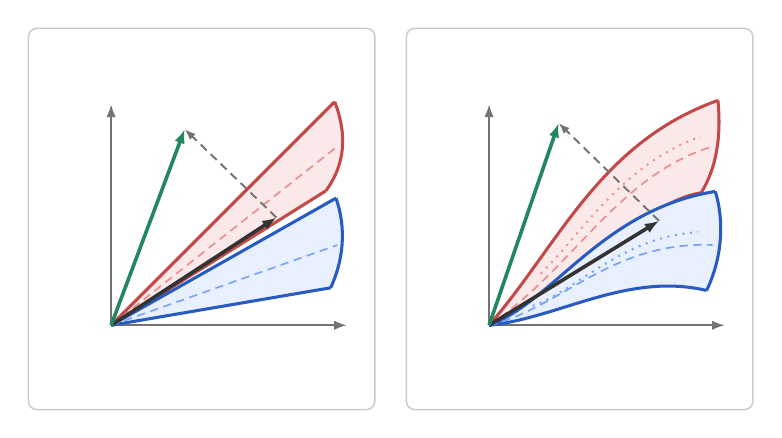
\begin{tikzpicture}
    \ifdefined\ONLYB
        \panelB
    \else
        \ifdefined\ONLYC
            \panelC
        \else
            \panelB
            \begin{scope}[xshift=4.80cm]
                \panelC
            \end{scope}
        \fi
    \fi
\end{tikzpicture}
\end{document}
'
%    xelatex -jobname=fig1_c_clean  '\def\ONLYC{}% ---------------------------------------------------------------------------
%  Figure 1 panels (b) and (c) -- TEXT-FREE export for PowerPoint.
%
%  Every label / annotation has been removed (panel titles, axis labels,
%  "$v_t^{cand}$", "$R_{1,\eta}$", "$VO^T_1$", origin "0", correction symbols,
%  the union equations ...).  Geometry, colours and line weights are identical
%  to the in-paper TikZ figure, so text can be re-added by hand in PPT.
%
%  Build from this folder:
%    xelatex -jobname=fig1_b_clean  '\def\ONLYB{}\input{fig1_bc_clean.tex}'
%    xelatex -jobname=fig1_c_clean  '\def\ONLYC{}\input{fig1_bc_clean.tex}'
%    xelatex -jobname=fig1_bc_clean '\input{fig1_bc_clean.tex}'
% ---------------------------------------------------------------------------
\documentclass[tikz,border=2pt]{standalone}

\usepackage{tikz}
\usetikzlibrary{arrows.meta,positioning,calc}

\definecolor{pvoBlue}{HTML}{2F6FED}
\definecolor{pvoGreen}{HTML}{2AA876}
\definecolor{pvoRed}{HTML}{E05252}

\tikzset{
    line join=round, line cap=round,
    panel/.style={rounded corners=3pt, draw=black!20, line width=0.55pt},
    axis/.style={-{Latex[length=1.6mm]}, line width=0.7pt, draw=black!55},
    riskone/.style={line width=1.1pt, draw=pvoRed!88!black},
    risktwo/.style={line width=1.1pt, draw=pvoBlue!82!black},
    meanline/.style={line width=0.62pt, densely dashed},
    candidate/.style={-{Latex[length=1.8mm]}, line width=1.3pt, draw=black!80},
    accepted/.style={-{Latex[length=1.8mm]}, line width=1.3pt, draw=pvoGreen!80!black},
    correction/.style={-{Latex[length=1.4mm]}, line width=0.7pt, densely dashed, draw=black!55}
}

% --------------------------------------------------------------- panel (b) --
\newcommand{\panelB}{%
    \draw[panel] (-0.10,-0.12) rectangle (4.30,4.72);
    \begin{scope}[shift={(0.95,0.95)}, scale=0.85, shift={(-0.48,-0.52)}]
        \draw[axis] (0.48,0.52) -- (4.00,0.52);
        \draw[axis] (0.48,0.52) -- (0.48,3.82);

        % deterministic relative-velocity cone for obstacle 1
        \path[fill=pvoRed!13]
            (0.48,0.52) -- (3.82,3.86)
            .. controls (4.01,3.37) and (3.98,2.93) .. (3.69,2.53) -- cycle;
        \draw[riskone] (0.48,0.52) -- (3.82,3.86);
        \draw[riskone] (0.48,0.52) -- (3.69,2.53);
        \draw[riskone] (3.82,3.86) .. controls (4.01,3.37) and (3.98,2.93) .. (3.69,2.53);
        \draw[meanline, pvoRed!64] (0.48,0.52) -- (3.82,3.16);

        % deterministic relative-velocity cone for obstacle 2
        \path[fill=pvoBlue!11]
            (0.48,0.52) -- (3.84,2.42)
            .. controls (4.00,1.96) and (3.95,1.49) .. (3.76,1.08) -- cycle;
        \draw[risktwo] (0.48,0.52) -- (3.84,2.42);
        \draw[risktwo] (0.48,0.52) -- (3.76,1.08);
        \draw[risktwo] (3.84,2.42) .. controls (4.00,1.96) and (3.95,1.49) .. (3.76,1.08);
        \draw[meanline, pvoBlue!62] (0.48,0.52) -- (3.86,1.72);

        % candidate velocity / filtered velocity / correction
        \draw[candidate] (0.48,0.52) -- (2.95,2.13);
        \draw[accepted] (0.48,0.52) -- (1.58,3.45);
        \draw[correction] (2.95,2.13) -- (1.58,3.45);
    \end{scope}%
}

% --------------------------------------------------------------- panel (c) --
\newcommand{\panelC}{%
    \draw[panel] (-0.10,-0.12) rectangle (4.30,4.72);
    \begin{scope}[shift={(0.95,0.95)}, scale=0.85, shift={(-0.48,-0.52)}]
        \draw[axis] (0.48,0.52) -- (4.00,0.52);
        \draw[axis] (0.48,0.52) -- (0.48,3.82);

        % action-conditioned risk tube for obstacle 1
        \path[fill=pvoRed!13]
            (0.48,0.52)
            .. controls (1.52,1.72) and (2.13,3.25) .. (3.90,3.88)
            .. controls (3.95,3.33) and (3.88,2.88) .. (3.65,2.50)
            .. controls (2.72,2.35) and (1.64,1.02) .. (0.48,0.52) -- cycle;
        \draw[riskone]
            (0.48,0.52) .. controls (1.52,1.72) and (2.13,3.25) .. (3.90,3.88);
        \draw[riskone]
            (0.48,0.52) .. controls (1.64,1.02) and (2.72,2.35) .. (3.65,2.50);
        \draw[riskone] (3.90,3.88) .. controls (3.95,3.33) and (3.88,2.88) .. (3.65,2.50);
        \draw[meanline, pvoRed!65]
            (0.48,0.52) .. controls (1.72,1.35) and (2.38,2.73) .. (3.78,3.18);
        \draw[dotted, line width=0.75pt, pvoRed!62]
            (1.25,1.29) .. controls (1.86,1.88) and (2.46,2.92) .. (3.64,3.34);

        % action-conditioned risk tube for obstacle 2
        \path[fill=pvoBlue!11]
            (0.48,0.52)
            .. controls (1.45,0.88) and (2.17,2.25) .. (3.86,2.52)
            .. controls (4.00,2.06) and (3.96,1.52) .. (3.73,1.04)
            .. controls (2.55,1.32) and (1.53,0.63) .. (0.48,0.52) -- cycle;
        \draw[risktwo]
            (0.48,0.52) .. controls (1.45,0.88) and (2.17,2.25) .. (3.86,2.52);
        \draw[risktwo]
            (0.48,0.52) .. controls (1.53,0.63) and (2.55,1.32) .. (3.73,1.04);
        \draw[risktwo] (3.86,2.52) .. controls (4.00,2.06) and (3.96,1.52) .. (3.73,1.04);
        \draw[meanline, pvoBlue!64]
            (0.48,0.52) .. controls (1.55,0.77) and (2.30,1.78) .. (3.82,1.72);
        \draw[dotted, line width=0.75pt, pvoBlue!62]
            (1.13,0.81) .. controls (1.79,1.04) and (2.48,1.85) .. (3.60,1.91);

        % candidate velocity / filtered velocity / correction
        \draw[candidate] (0.48,0.52) -- (3.02,2.08);
        \draw[accepted] (0.48,0.52) -- (1.52,3.54);
        \draw[correction] (3.02,2.08) -- (1.52,3.54);
    \end{scope}%
}

\begin{document}
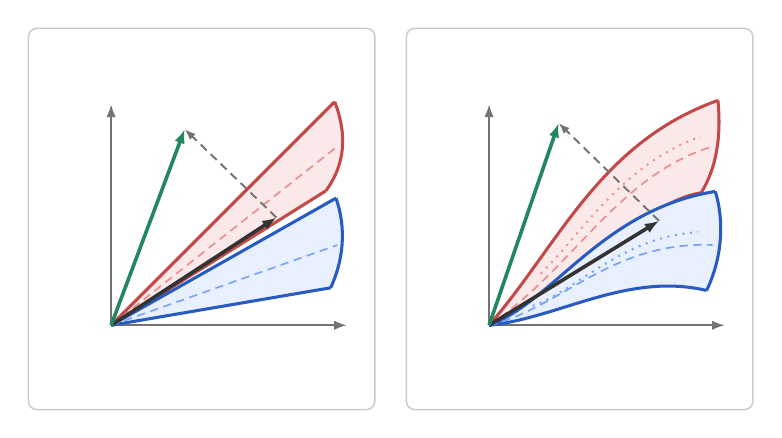
\begin{tikzpicture}
    \ifdefined\ONLYB
        \panelB
    \else
        \ifdefined\ONLYC
            \panelC
        \else
            \panelB
            \begin{scope}[xshift=4.80cm]
                \panelC
            \end{scope}
        \fi
    \fi
\end{tikzpicture}
\end{document}
'
%    xelatex -jobname=fig1_bc_clean '% ---------------------------------------------------------------------------
%  Figure 1 panels (b) and (c) -- TEXT-FREE export for PowerPoint.
%
%  Every label / annotation has been removed (panel titles, axis labels,
%  "$v_t^{cand}$", "$R_{1,\eta}$", "$VO^T_1$", origin "0", correction symbols,
%  the union equations ...).  Geometry, colours and line weights are identical
%  to the in-paper TikZ figure, so text can be re-added by hand in PPT.
%
%  Build from this folder:
%    xelatex -jobname=fig1_b_clean  '\def\ONLYB{}\input{fig1_bc_clean.tex}'
%    xelatex -jobname=fig1_c_clean  '\def\ONLYC{}\input{fig1_bc_clean.tex}'
%    xelatex -jobname=fig1_bc_clean '\input{fig1_bc_clean.tex}'
% ---------------------------------------------------------------------------
\documentclass[tikz,border=2pt]{standalone}

\usepackage{tikz}
\usetikzlibrary{arrows.meta,positioning,calc}

\definecolor{pvoBlue}{HTML}{2F6FED}
\definecolor{pvoGreen}{HTML}{2AA876}
\definecolor{pvoRed}{HTML}{E05252}

\tikzset{
    line join=round, line cap=round,
    panel/.style={rounded corners=3pt, draw=black!20, line width=0.55pt},
    axis/.style={-{Latex[length=1.6mm]}, line width=0.7pt, draw=black!55},
    riskone/.style={line width=1.1pt, draw=pvoRed!88!black},
    risktwo/.style={line width=1.1pt, draw=pvoBlue!82!black},
    meanline/.style={line width=0.62pt, densely dashed},
    candidate/.style={-{Latex[length=1.8mm]}, line width=1.3pt, draw=black!80},
    accepted/.style={-{Latex[length=1.8mm]}, line width=1.3pt, draw=pvoGreen!80!black},
    correction/.style={-{Latex[length=1.4mm]}, line width=0.7pt, densely dashed, draw=black!55}
}

% --------------------------------------------------------------- panel (b) --
\newcommand{\panelB}{%
    \draw[panel] (-0.10,-0.12) rectangle (4.30,4.72);
    \begin{scope}[shift={(0.95,0.95)}, scale=0.85, shift={(-0.48,-0.52)}]
        \draw[axis] (0.48,0.52) -- (4.00,0.52);
        \draw[axis] (0.48,0.52) -- (0.48,3.82);

        % deterministic relative-velocity cone for obstacle 1
        \path[fill=pvoRed!13]
            (0.48,0.52) -- (3.82,3.86)
            .. controls (4.01,3.37) and (3.98,2.93) .. (3.69,2.53) -- cycle;
        \draw[riskone] (0.48,0.52) -- (3.82,3.86);
        \draw[riskone] (0.48,0.52) -- (3.69,2.53);
        \draw[riskone] (3.82,3.86) .. controls (4.01,3.37) and (3.98,2.93) .. (3.69,2.53);
        \draw[meanline, pvoRed!64] (0.48,0.52) -- (3.82,3.16);

        % deterministic relative-velocity cone for obstacle 2
        \path[fill=pvoBlue!11]
            (0.48,0.52) -- (3.84,2.42)
            .. controls (4.00,1.96) and (3.95,1.49) .. (3.76,1.08) -- cycle;
        \draw[risktwo] (0.48,0.52) -- (3.84,2.42);
        \draw[risktwo] (0.48,0.52) -- (3.76,1.08);
        \draw[risktwo] (3.84,2.42) .. controls (4.00,1.96) and (3.95,1.49) .. (3.76,1.08);
        \draw[meanline, pvoBlue!62] (0.48,0.52) -- (3.86,1.72);

        % candidate velocity / filtered velocity / correction
        \draw[candidate] (0.48,0.52) -- (2.95,2.13);
        \draw[accepted] (0.48,0.52) -- (1.58,3.45);
        \draw[correction] (2.95,2.13) -- (1.58,3.45);
    \end{scope}%
}

% --------------------------------------------------------------- panel (c) --
\newcommand{\panelC}{%
    \draw[panel] (-0.10,-0.12) rectangle (4.30,4.72);
    \begin{scope}[shift={(0.95,0.95)}, scale=0.85, shift={(-0.48,-0.52)}]
        \draw[axis] (0.48,0.52) -- (4.00,0.52);
        \draw[axis] (0.48,0.52) -- (0.48,3.82);

        % action-conditioned risk tube for obstacle 1
        \path[fill=pvoRed!13]
            (0.48,0.52)
            .. controls (1.52,1.72) and (2.13,3.25) .. (3.90,3.88)
            .. controls (3.95,3.33) and (3.88,2.88) .. (3.65,2.50)
            .. controls (2.72,2.35) and (1.64,1.02) .. (0.48,0.52) -- cycle;
        \draw[riskone]
            (0.48,0.52) .. controls (1.52,1.72) and (2.13,3.25) .. (3.90,3.88);
        \draw[riskone]
            (0.48,0.52) .. controls (1.64,1.02) and (2.72,2.35) .. (3.65,2.50);
        \draw[riskone] (3.90,3.88) .. controls (3.95,3.33) and (3.88,2.88) .. (3.65,2.50);
        \draw[meanline, pvoRed!65]
            (0.48,0.52) .. controls (1.72,1.35) and (2.38,2.73) .. (3.78,3.18);
        \draw[dotted, line width=0.75pt, pvoRed!62]
            (1.25,1.29) .. controls (1.86,1.88) and (2.46,2.92) .. (3.64,3.34);

        % action-conditioned risk tube for obstacle 2
        \path[fill=pvoBlue!11]
            (0.48,0.52)
            .. controls (1.45,0.88) and (2.17,2.25) .. (3.86,2.52)
            .. controls (4.00,2.06) and (3.96,1.52) .. (3.73,1.04)
            .. controls (2.55,1.32) and (1.53,0.63) .. (0.48,0.52) -- cycle;
        \draw[risktwo]
            (0.48,0.52) .. controls (1.45,0.88) and (2.17,2.25) .. (3.86,2.52);
        \draw[risktwo]
            (0.48,0.52) .. controls (1.53,0.63) and (2.55,1.32) .. (3.73,1.04);
        \draw[risktwo] (3.86,2.52) .. controls (4.00,2.06) and (3.96,1.52) .. (3.73,1.04);
        \draw[meanline, pvoBlue!64]
            (0.48,0.52) .. controls (1.55,0.77) and (2.30,1.78) .. (3.82,1.72);
        \draw[dotted, line width=0.75pt, pvoBlue!62]
            (1.13,0.81) .. controls (1.79,1.04) and (2.48,1.85) .. (3.60,1.91);

        % candidate velocity / filtered velocity / correction
        \draw[candidate] (0.48,0.52) -- (3.02,2.08);
        \draw[accepted] (0.48,0.52) -- (1.52,3.54);
        \draw[correction] (3.02,2.08) -- (1.52,3.54);
    \end{scope}%
}

\begin{document}
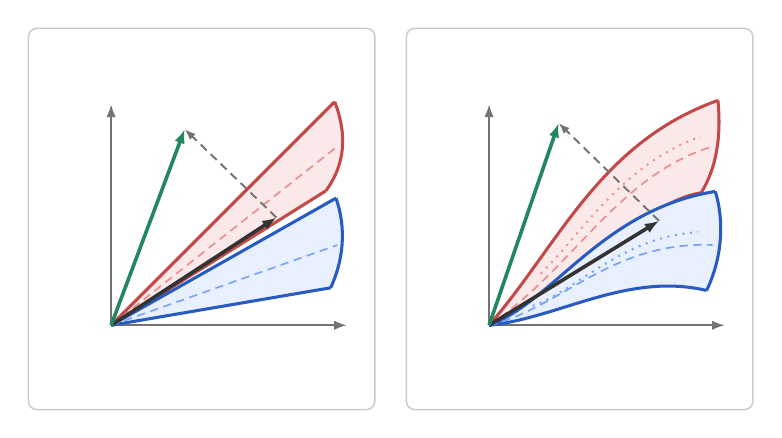
\begin{tikzpicture}
    \ifdefined\ONLYB
        \panelB
    \else
        \ifdefined\ONLYC
            \panelC
        \else
            \panelB
            \begin{scope}[xshift=4.80cm]
                \panelC
            \end{scope}
        \fi
    \fi
\end{tikzpicture}
\end{document}
'
% ---------------------------------------------------------------------------
\documentclass[tikz,border=2pt]{standalone}

\usepackage{tikz}
\usetikzlibrary{arrows.meta,positioning,calc}

\definecolor{pvoBlue}{HTML}{2F6FED}
\definecolor{pvoGreen}{HTML}{2AA876}
\definecolor{pvoRed}{HTML}{E05252}

\tikzset{
    line join=round, line cap=round,
    panel/.style={rounded corners=3pt, draw=black!20, line width=0.55pt},
    axis/.style={-{Latex[length=1.6mm]}, line width=0.7pt, draw=black!55},
    riskone/.style={line width=1.1pt, draw=pvoRed!88!black},
    risktwo/.style={line width=1.1pt, draw=pvoBlue!82!black},
    meanline/.style={line width=0.62pt, densely dashed},
    candidate/.style={-{Latex[length=1.8mm]}, line width=1.3pt, draw=black!80},
    accepted/.style={-{Latex[length=1.8mm]}, line width=1.3pt, draw=pvoGreen!80!black},
    correction/.style={-{Latex[length=1.4mm]}, line width=0.7pt, densely dashed, draw=black!55}
}

% --------------------------------------------------------------- panel (b) --
\newcommand{\panelB}{%
    \draw[panel] (-0.10,-0.12) rectangle (4.30,4.72);
    \begin{scope}[shift={(0.95,0.95)}, scale=0.85, shift={(-0.48,-0.52)}]
        \draw[axis] (0.48,0.52) -- (4.00,0.52);
        \draw[axis] (0.48,0.52) -- (0.48,3.82);

        % deterministic relative-velocity cone for obstacle 1
        \path[fill=pvoRed!13]
            (0.48,0.52) -- (3.82,3.86)
            .. controls (4.01,3.37) and (3.98,2.93) .. (3.69,2.53) -- cycle;
        \draw[riskone] (0.48,0.52) -- (3.82,3.86);
        \draw[riskone] (0.48,0.52) -- (3.69,2.53);
        \draw[riskone] (3.82,3.86) .. controls (4.01,3.37) and (3.98,2.93) .. (3.69,2.53);
        \draw[meanline, pvoRed!64] (0.48,0.52) -- (3.82,3.16);

        % deterministic relative-velocity cone for obstacle 2
        \path[fill=pvoBlue!11]
            (0.48,0.52) -- (3.84,2.42)
            .. controls (4.00,1.96) and (3.95,1.49) .. (3.76,1.08) -- cycle;
        \draw[risktwo] (0.48,0.52) -- (3.84,2.42);
        \draw[risktwo] (0.48,0.52) -- (3.76,1.08);
        \draw[risktwo] (3.84,2.42) .. controls (4.00,1.96) and (3.95,1.49) .. (3.76,1.08);
        \draw[meanline, pvoBlue!62] (0.48,0.52) -- (3.86,1.72);

        % candidate velocity / filtered velocity / correction
        \draw[candidate] (0.48,0.52) -- (2.95,2.13);
        \draw[accepted] (0.48,0.52) -- (1.58,3.45);
        \draw[correction] (2.95,2.13) -- (1.58,3.45);
    \end{scope}%
}

% --------------------------------------------------------------- panel (c) --
\newcommand{\panelC}{%
    \draw[panel] (-0.10,-0.12) rectangle (4.30,4.72);
    \begin{scope}[shift={(0.95,0.95)}, scale=0.85, shift={(-0.48,-0.52)}]
        \draw[axis] (0.48,0.52) -- (4.00,0.52);
        \draw[axis] (0.48,0.52) -- (0.48,3.82);

        % action-conditioned risk tube for obstacle 1
        \path[fill=pvoRed!13]
            (0.48,0.52)
            .. controls (1.52,1.72) and (2.13,3.25) .. (3.90,3.88)
            .. controls (3.95,3.33) and (3.88,2.88) .. (3.65,2.50)
            .. controls (2.72,2.35) and (1.64,1.02) .. (0.48,0.52) -- cycle;
        \draw[riskone]
            (0.48,0.52) .. controls (1.52,1.72) and (2.13,3.25) .. (3.90,3.88);
        \draw[riskone]
            (0.48,0.52) .. controls (1.64,1.02) and (2.72,2.35) .. (3.65,2.50);
        \draw[riskone] (3.90,3.88) .. controls (3.95,3.33) and (3.88,2.88) .. (3.65,2.50);
        \draw[meanline, pvoRed!65]
            (0.48,0.52) .. controls (1.72,1.35) and (2.38,2.73) .. (3.78,3.18);
        \draw[dotted, line width=0.75pt, pvoRed!62]
            (1.25,1.29) .. controls (1.86,1.88) and (2.46,2.92) .. (3.64,3.34);

        % action-conditioned risk tube for obstacle 2
        \path[fill=pvoBlue!11]
            (0.48,0.52)
            .. controls (1.45,0.88) and (2.17,2.25) .. (3.86,2.52)
            .. controls (4.00,2.06) and (3.96,1.52) .. (3.73,1.04)
            .. controls (2.55,1.32) and (1.53,0.63) .. (0.48,0.52) -- cycle;
        \draw[risktwo]
            (0.48,0.52) .. controls (1.45,0.88) and (2.17,2.25) .. (3.86,2.52);
        \draw[risktwo]
            (0.48,0.52) .. controls (1.53,0.63) and (2.55,1.32) .. (3.73,1.04);
        \draw[risktwo] (3.86,2.52) .. controls (4.00,2.06) and (3.96,1.52) .. (3.73,1.04);
        \draw[meanline, pvoBlue!64]
            (0.48,0.52) .. controls (1.55,0.77) and (2.30,1.78) .. (3.82,1.72);
        \draw[dotted, line width=0.75pt, pvoBlue!62]
            (1.13,0.81) .. controls (1.79,1.04) and (2.48,1.85) .. (3.60,1.91);

        % candidate velocity / filtered velocity / correction
        \draw[candidate] (0.48,0.52) -- (3.02,2.08);
        \draw[accepted] (0.48,0.52) -- (1.52,3.54);
        \draw[correction] (3.02,2.08) -- (1.52,3.54);
    \end{scope}%
}

\begin{document}
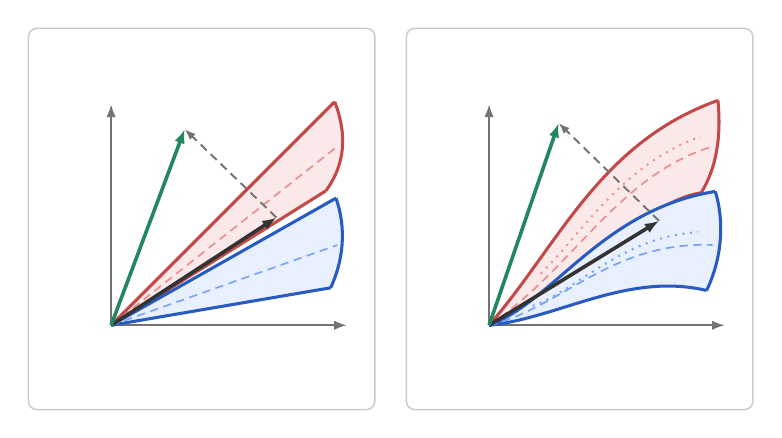
\begin{tikzpicture}
    \ifdefined\ONLYB
        \panelB
    \else
        \ifdefined\ONLYC
            \panelC
        \else
            \panelB
            \begin{scope}[xshift=4.80cm]
                \panelC
            \end{scope}
        \fi
    \fi
\end{tikzpicture}
\end{document}
'
%    xelatex -jobname=fig1_bc_clean '% ---------------------------------------------------------------------------
%  Figure 1 panels (b) and (c) -- TEXT-FREE export for PowerPoint.
%
%  Every label / annotation has been removed (panel titles, axis labels,
%  "$v_t^{cand}$", "$R_{1,\eta}$", "$VO^T_1$", origin "0", correction symbols,
%  the union equations ...).  Geometry, colours and line weights are identical
%  to the in-paper TikZ figure, so text can be re-added by hand in PPT.
%
%  Build from this folder:
%    xelatex -jobname=fig1_b_clean  '\def\ONLYB{}% ---------------------------------------------------------------------------
%  Figure 1 panels (b) and (c) -- TEXT-FREE export for PowerPoint.
%
%  Every label / annotation has been removed (panel titles, axis labels,
%  "$v_t^{cand}$", "$R_{1,\eta}$", "$VO^T_1$", origin "0", correction symbols,
%  the union equations ...).  Geometry, colours and line weights are identical
%  to the in-paper TikZ figure, so text can be re-added by hand in PPT.
%
%  Build from this folder:
%    xelatex -jobname=fig1_b_clean  '\def\ONLYB{}\input{fig1_bc_clean.tex}'
%    xelatex -jobname=fig1_c_clean  '\def\ONLYC{}\input{fig1_bc_clean.tex}'
%    xelatex -jobname=fig1_bc_clean '\input{fig1_bc_clean.tex}'
% ---------------------------------------------------------------------------
\documentclass[tikz,border=2pt]{standalone}

\usepackage{tikz}
\usetikzlibrary{arrows.meta,positioning,calc}

\definecolor{pvoBlue}{HTML}{2F6FED}
\definecolor{pvoGreen}{HTML}{2AA876}
\definecolor{pvoRed}{HTML}{E05252}

\tikzset{
    line join=round, line cap=round,
    panel/.style={rounded corners=3pt, draw=black!20, line width=0.55pt},
    axis/.style={-{Latex[length=1.6mm]}, line width=0.7pt, draw=black!55},
    riskone/.style={line width=1.1pt, draw=pvoRed!88!black},
    risktwo/.style={line width=1.1pt, draw=pvoBlue!82!black},
    meanline/.style={line width=0.62pt, densely dashed},
    candidate/.style={-{Latex[length=1.8mm]}, line width=1.3pt, draw=black!80},
    accepted/.style={-{Latex[length=1.8mm]}, line width=1.3pt, draw=pvoGreen!80!black},
    correction/.style={-{Latex[length=1.4mm]}, line width=0.7pt, densely dashed, draw=black!55}
}

% --------------------------------------------------------------- panel (b) --
\newcommand{\panelB}{%
    \draw[panel] (-0.10,-0.12) rectangle (4.30,4.72);
    \begin{scope}[shift={(0.95,0.95)}, scale=0.85, shift={(-0.48,-0.52)}]
        \draw[axis] (0.48,0.52) -- (4.00,0.52);
        \draw[axis] (0.48,0.52) -- (0.48,3.82);

        % deterministic relative-velocity cone for obstacle 1
        \path[fill=pvoRed!13]
            (0.48,0.52) -- (3.82,3.86)
            .. controls (4.01,3.37) and (3.98,2.93) .. (3.69,2.53) -- cycle;
        \draw[riskone] (0.48,0.52) -- (3.82,3.86);
        \draw[riskone] (0.48,0.52) -- (3.69,2.53);
        \draw[riskone] (3.82,3.86) .. controls (4.01,3.37) and (3.98,2.93) .. (3.69,2.53);
        \draw[meanline, pvoRed!64] (0.48,0.52) -- (3.82,3.16);

        % deterministic relative-velocity cone for obstacle 2
        \path[fill=pvoBlue!11]
            (0.48,0.52) -- (3.84,2.42)
            .. controls (4.00,1.96) and (3.95,1.49) .. (3.76,1.08) -- cycle;
        \draw[risktwo] (0.48,0.52) -- (3.84,2.42);
        \draw[risktwo] (0.48,0.52) -- (3.76,1.08);
        \draw[risktwo] (3.84,2.42) .. controls (4.00,1.96) and (3.95,1.49) .. (3.76,1.08);
        \draw[meanline, pvoBlue!62] (0.48,0.52) -- (3.86,1.72);

        % candidate velocity / filtered velocity / correction
        \draw[candidate] (0.48,0.52) -- (2.95,2.13);
        \draw[accepted] (0.48,0.52) -- (1.58,3.45);
        \draw[correction] (2.95,2.13) -- (1.58,3.45);
    \end{scope}%
}

% --------------------------------------------------------------- panel (c) --
\newcommand{\panelC}{%
    \draw[panel] (-0.10,-0.12) rectangle (4.30,4.72);
    \begin{scope}[shift={(0.95,0.95)}, scale=0.85, shift={(-0.48,-0.52)}]
        \draw[axis] (0.48,0.52) -- (4.00,0.52);
        \draw[axis] (0.48,0.52) -- (0.48,3.82);

        % action-conditioned risk tube for obstacle 1
        \path[fill=pvoRed!13]
            (0.48,0.52)
            .. controls (1.52,1.72) and (2.13,3.25) .. (3.90,3.88)
            .. controls (3.95,3.33) and (3.88,2.88) .. (3.65,2.50)
            .. controls (2.72,2.35) and (1.64,1.02) .. (0.48,0.52) -- cycle;
        \draw[riskone]
            (0.48,0.52) .. controls (1.52,1.72) and (2.13,3.25) .. (3.90,3.88);
        \draw[riskone]
            (0.48,0.52) .. controls (1.64,1.02) and (2.72,2.35) .. (3.65,2.50);
        \draw[riskone] (3.90,3.88) .. controls (3.95,3.33) and (3.88,2.88) .. (3.65,2.50);
        \draw[meanline, pvoRed!65]
            (0.48,0.52) .. controls (1.72,1.35) and (2.38,2.73) .. (3.78,3.18);
        \draw[dotted, line width=0.75pt, pvoRed!62]
            (1.25,1.29) .. controls (1.86,1.88) and (2.46,2.92) .. (3.64,3.34);

        % action-conditioned risk tube for obstacle 2
        \path[fill=pvoBlue!11]
            (0.48,0.52)
            .. controls (1.45,0.88) and (2.17,2.25) .. (3.86,2.52)
            .. controls (4.00,2.06) and (3.96,1.52) .. (3.73,1.04)
            .. controls (2.55,1.32) and (1.53,0.63) .. (0.48,0.52) -- cycle;
        \draw[risktwo]
            (0.48,0.52) .. controls (1.45,0.88) and (2.17,2.25) .. (3.86,2.52);
        \draw[risktwo]
            (0.48,0.52) .. controls (1.53,0.63) and (2.55,1.32) .. (3.73,1.04);
        \draw[risktwo] (3.86,2.52) .. controls (4.00,2.06) and (3.96,1.52) .. (3.73,1.04);
        \draw[meanline, pvoBlue!64]
            (0.48,0.52) .. controls (1.55,0.77) and (2.30,1.78) .. (3.82,1.72);
        \draw[dotted, line width=0.75pt, pvoBlue!62]
            (1.13,0.81) .. controls (1.79,1.04) and (2.48,1.85) .. (3.60,1.91);

        % candidate velocity / filtered velocity / correction
        \draw[candidate] (0.48,0.52) -- (3.02,2.08);
        \draw[accepted] (0.48,0.52) -- (1.52,3.54);
        \draw[correction] (3.02,2.08) -- (1.52,3.54);
    \end{scope}%
}

\begin{document}
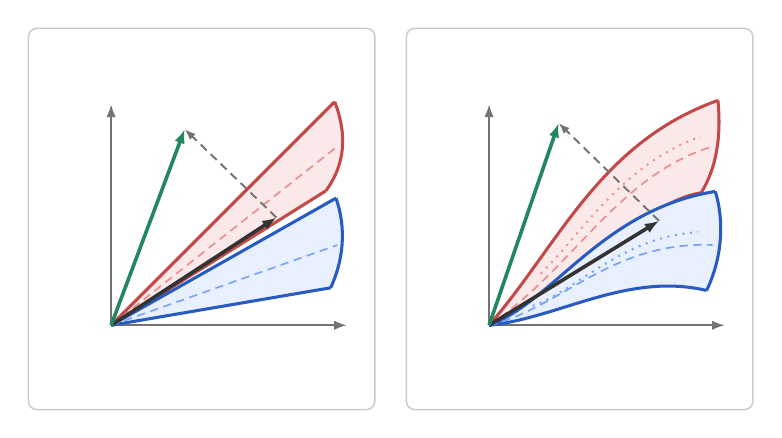
\begin{tikzpicture}
    \ifdefined\ONLYB
        \panelB
    \else
        \ifdefined\ONLYC
            \panelC
        \else
            \panelB
            \begin{scope}[xshift=4.80cm]
                \panelC
            \end{scope}
        \fi
    \fi
\end{tikzpicture}
\end{document}
'
%    xelatex -jobname=fig1_c_clean  '\def\ONLYC{}% ---------------------------------------------------------------------------
%  Figure 1 panels (b) and (c) -- TEXT-FREE export for PowerPoint.
%
%  Every label / annotation has been removed (panel titles, axis labels,
%  "$v_t^{cand}$", "$R_{1,\eta}$", "$VO^T_1$", origin "0", correction symbols,
%  the union equations ...).  Geometry, colours and line weights are identical
%  to the in-paper TikZ figure, so text can be re-added by hand in PPT.
%
%  Build from this folder:
%    xelatex -jobname=fig1_b_clean  '\def\ONLYB{}\input{fig1_bc_clean.tex}'
%    xelatex -jobname=fig1_c_clean  '\def\ONLYC{}\input{fig1_bc_clean.tex}'
%    xelatex -jobname=fig1_bc_clean '\input{fig1_bc_clean.tex}'
% ---------------------------------------------------------------------------
\documentclass[tikz,border=2pt]{standalone}

\usepackage{tikz}
\usetikzlibrary{arrows.meta,positioning,calc}

\definecolor{pvoBlue}{HTML}{2F6FED}
\definecolor{pvoGreen}{HTML}{2AA876}
\definecolor{pvoRed}{HTML}{E05252}

\tikzset{
    line join=round, line cap=round,
    panel/.style={rounded corners=3pt, draw=black!20, line width=0.55pt},
    axis/.style={-{Latex[length=1.6mm]}, line width=0.7pt, draw=black!55},
    riskone/.style={line width=1.1pt, draw=pvoRed!88!black},
    risktwo/.style={line width=1.1pt, draw=pvoBlue!82!black},
    meanline/.style={line width=0.62pt, densely dashed},
    candidate/.style={-{Latex[length=1.8mm]}, line width=1.3pt, draw=black!80},
    accepted/.style={-{Latex[length=1.8mm]}, line width=1.3pt, draw=pvoGreen!80!black},
    correction/.style={-{Latex[length=1.4mm]}, line width=0.7pt, densely dashed, draw=black!55}
}

% --------------------------------------------------------------- panel (b) --
\newcommand{\panelB}{%
    \draw[panel] (-0.10,-0.12) rectangle (4.30,4.72);
    \begin{scope}[shift={(0.95,0.95)}, scale=0.85, shift={(-0.48,-0.52)}]
        \draw[axis] (0.48,0.52) -- (4.00,0.52);
        \draw[axis] (0.48,0.52) -- (0.48,3.82);

        % deterministic relative-velocity cone for obstacle 1
        \path[fill=pvoRed!13]
            (0.48,0.52) -- (3.82,3.86)
            .. controls (4.01,3.37) and (3.98,2.93) .. (3.69,2.53) -- cycle;
        \draw[riskone] (0.48,0.52) -- (3.82,3.86);
        \draw[riskone] (0.48,0.52) -- (3.69,2.53);
        \draw[riskone] (3.82,3.86) .. controls (4.01,3.37) and (3.98,2.93) .. (3.69,2.53);
        \draw[meanline, pvoRed!64] (0.48,0.52) -- (3.82,3.16);

        % deterministic relative-velocity cone for obstacle 2
        \path[fill=pvoBlue!11]
            (0.48,0.52) -- (3.84,2.42)
            .. controls (4.00,1.96) and (3.95,1.49) .. (3.76,1.08) -- cycle;
        \draw[risktwo] (0.48,0.52) -- (3.84,2.42);
        \draw[risktwo] (0.48,0.52) -- (3.76,1.08);
        \draw[risktwo] (3.84,2.42) .. controls (4.00,1.96) and (3.95,1.49) .. (3.76,1.08);
        \draw[meanline, pvoBlue!62] (0.48,0.52) -- (3.86,1.72);

        % candidate velocity / filtered velocity / correction
        \draw[candidate] (0.48,0.52) -- (2.95,2.13);
        \draw[accepted] (0.48,0.52) -- (1.58,3.45);
        \draw[correction] (2.95,2.13) -- (1.58,3.45);
    \end{scope}%
}

% --------------------------------------------------------------- panel (c) --
\newcommand{\panelC}{%
    \draw[panel] (-0.10,-0.12) rectangle (4.30,4.72);
    \begin{scope}[shift={(0.95,0.95)}, scale=0.85, shift={(-0.48,-0.52)}]
        \draw[axis] (0.48,0.52) -- (4.00,0.52);
        \draw[axis] (0.48,0.52) -- (0.48,3.82);

        % action-conditioned risk tube for obstacle 1
        \path[fill=pvoRed!13]
            (0.48,0.52)
            .. controls (1.52,1.72) and (2.13,3.25) .. (3.90,3.88)
            .. controls (3.95,3.33) and (3.88,2.88) .. (3.65,2.50)
            .. controls (2.72,2.35) and (1.64,1.02) .. (0.48,0.52) -- cycle;
        \draw[riskone]
            (0.48,0.52) .. controls (1.52,1.72) and (2.13,3.25) .. (3.90,3.88);
        \draw[riskone]
            (0.48,0.52) .. controls (1.64,1.02) and (2.72,2.35) .. (3.65,2.50);
        \draw[riskone] (3.90,3.88) .. controls (3.95,3.33) and (3.88,2.88) .. (3.65,2.50);
        \draw[meanline, pvoRed!65]
            (0.48,0.52) .. controls (1.72,1.35) and (2.38,2.73) .. (3.78,3.18);
        \draw[dotted, line width=0.75pt, pvoRed!62]
            (1.25,1.29) .. controls (1.86,1.88) and (2.46,2.92) .. (3.64,3.34);

        % action-conditioned risk tube for obstacle 2
        \path[fill=pvoBlue!11]
            (0.48,0.52)
            .. controls (1.45,0.88) and (2.17,2.25) .. (3.86,2.52)
            .. controls (4.00,2.06) and (3.96,1.52) .. (3.73,1.04)
            .. controls (2.55,1.32) and (1.53,0.63) .. (0.48,0.52) -- cycle;
        \draw[risktwo]
            (0.48,0.52) .. controls (1.45,0.88) and (2.17,2.25) .. (3.86,2.52);
        \draw[risktwo]
            (0.48,0.52) .. controls (1.53,0.63) and (2.55,1.32) .. (3.73,1.04);
        \draw[risktwo] (3.86,2.52) .. controls (4.00,2.06) and (3.96,1.52) .. (3.73,1.04);
        \draw[meanline, pvoBlue!64]
            (0.48,0.52) .. controls (1.55,0.77) and (2.30,1.78) .. (3.82,1.72);
        \draw[dotted, line width=0.75pt, pvoBlue!62]
            (1.13,0.81) .. controls (1.79,1.04) and (2.48,1.85) .. (3.60,1.91);

        % candidate velocity / filtered velocity / correction
        \draw[candidate] (0.48,0.52) -- (3.02,2.08);
        \draw[accepted] (0.48,0.52) -- (1.52,3.54);
        \draw[correction] (3.02,2.08) -- (1.52,3.54);
    \end{scope}%
}

\begin{document}
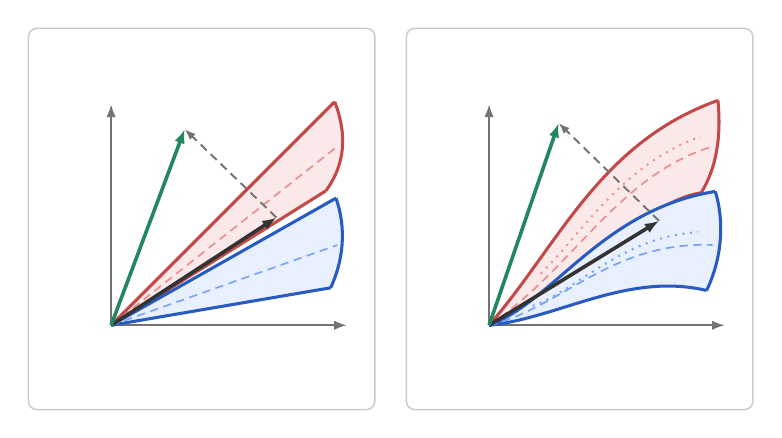
\begin{tikzpicture}
    \ifdefined\ONLYB
        \panelB
    \else
        \ifdefined\ONLYC
            \panelC
        \else
            \panelB
            \begin{scope}[xshift=4.80cm]
                \panelC
            \end{scope}
        \fi
    \fi
\end{tikzpicture}
\end{document}
'
%    xelatex -jobname=fig1_bc_clean '% ---------------------------------------------------------------------------
%  Figure 1 panels (b) and (c) -- TEXT-FREE export for PowerPoint.
%
%  Every label / annotation has been removed (panel titles, axis labels,
%  "$v_t^{cand}$", "$R_{1,\eta}$", "$VO^T_1$", origin "0", correction symbols,
%  the union equations ...).  Geometry, colours and line weights are identical
%  to the in-paper TikZ figure, so text can be re-added by hand in PPT.
%
%  Build from this folder:
%    xelatex -jobname=fig1_b_clean  '\def\ONLYB{}\input{fig1_bc_clean.tex}'
%    xelatex -jobname=fig1_c_clean  '\def\ONLYC{}\input{fig1_bc_clean.tex}'
%    xelatex -jobname=fig1_bc_clean '\input{fig1_bc_clean.tex}'
% ---------------------------------------------------------------------------
\documentclass[tikz,border=2pt]{standalone}

\usepackage{tikz}
\usetikzlibrary{arrows.meta,positioning,calc}

\definecolor{pvoBlue}{HTML}{2F6FED}
\definecolor{pvoGreen}{HTML}{2AA876}
\definecolor{pvoRed}{HTML}{E05252}

\tikzset{
    line join=round, line cap=round,
    panel/.style={rounded corners=3pt, draw=black!20, line width=0.55pt},
    axis/.style={-{Latex[length=1.6mm]}, line width=0.7pt, draw=black!55},
    riskone/.style={line width=1.1pt, draw=pvoRed!88!black},
    risktwo/.style={line width=1.1pt, draw=pvoBlue!82!black},
    meanline/.style={line width=0.62pt, densely dashed},
    candidate/.style={-{Latex[length=1.8mm]}, line width=1.3pt, draw=black!80},
    accepted/.style={-{Latex[length=1.8mm]}, line width=1.3pt, draw=pvoGreen!80!black},
    correction/.style={-{Latex[length=1.4mm]}, line width=0.7pt, densely dashed, draw=black!55}
}

% --------------------------------------------------------------- panel (b) --
\newcommand{\panelB}{%
    \draw[panel] (-0.10,-0.12) rectangle (4.30,4.72);
    \begin{scope}[shift={(0.95,0.95)}, scale=0.85, shift={(-0.48,-0.52)}]
        \draw[axis] (0.48,0.52) -- (4.00,0.52);
        \draw[axis] (0.48,0.52) -- (0.48,3.82);

        % deterministic relative-velocity cone for obstacle 1
        \path[fill=pvoRed!13]
            (0.48,0.52) -- (3.82,3.86)
            .. controls (4.01,3.37) and (3.98,2.93) .. (3.69,2.53) -- cycle;
        \draw[riskone] (0.48,0.52) -- (3.82,3.86);
        \draw[riskone] (0.48,0.52) -- (3.69,2.53);
        \draw[riskone] (3.82,3.86) .. controls (4.01,3.37) and (3.98,2.93) .. (3.69,2.53);
        \draw[meanline, pvoRed!64] (0.48,0.52) -- (3.82,3.16);

        % deterministic relative-velocity cone for obstacle 2
        \path[fill=pvoBlue!11]
            (0.48,0.52) -- (3.84,2.42)
            .. controls (4.00,1.96) and (3.95,1.49) .. (3.76,1.08) -- cycle;
        \draw[risktwo] (0.48,0.52) -- (3.84,2.42);
        \draw[risktwo] (0.48,0.52) -- (3.76,1.08);
        \draw[risktwo] (3.84,2.42) .. controls (4.00,1.96) and (3.95,1.49) .. (3.76,1.08);
        \draw[meanline, pvoBlue!62] (0.48,0.52) -- (3.86,1.72);

        % candidate velocity / filtered velocity / correction
        \draw[candidate] (0.48,0.52) -- (2.95,2.13);
        \draw[accepted] (0.48,0.52) -- (1.58,3.45);
        \draw[correction] (2.95,2.13) -- (1.58,3.45);
    \end{scope}%
}

% --------------------------------------------------------------- panel (c) --
\newcommand{\panelC}{%
    \draw[panel] (-0.10,-0.12) rectangle (4.30,4.72);
    \begin{scope}[shift={(0.95,0.95)}, scale=0.85, shift={(-0.48,-0.52)}]
        \draw[axis] (0.48,0.52) -- (4.00,0.52);
        \draw[axis] (0.48,0.52) -- (0.48,3.82);

        % action-conditioned risk tube for obstacle 1
        \path[fill=pvoRed!13]
            (0.48,0.52)
            .. controls (1.52,1.72) and (2.13,3.25) .. (3.90,3.88)
            .. controls (3.95,3.33) and (3.88,2.88) .. (3.65,2.50)
            .. controls (2.72,2.35) and (1.64,1.02) .. (0.48,0.52) -- cycle;
        \draw[riskone]
            (0.48,0.52) .. controls (1.52,1.72) and (2.13,3.25) .. (3.90,3.88);
        \draw[riskone]
            (0.48,0.52) .. controls (1.64,1.02) and (2.72,2.35) .. (3.65,2.50);
        \draw[riskone] (3.90,3.88) .. controls (3.95,3.33) and (3.88,2.88) .. (3.65,2.50);
        \draw[meanline, pvoRed!65]
            (0.48,0.52) .. controls (1.72,1.35) and (2.38,2.73) .. (3.78,3.18);
        \draw[dotted, line width=0.75pt, pvoRed!62]
            (1.25,1.29) .. controls (1.86,1.88) and (2.46,2.92) .. (3.64,3.34);

        % action-conditioned risk tube for obstacle 2
        \path[fill=pvoBlue!11]
            (0.48,0.52)
            .. controls (1.45,0.88) and (2.17,2.25) .. (3.86,2.52)
            .. controls (4.00,2.06) and (3.96,1.52) .. (3.73,1.04)
            .. controls (2.55,1.32) and (1.53,0.63) .. (0.48,0.52) -- cycle;
        \draw[risktwo]
            (0.48,0.52) .. controls (1.45,0.88) and (2.17,2.25) .. (3.86,2.52);
        \draw[risktwo]
            (0.48,0.52) .. controls (1.53,0.63) and (2.55,1.32) .. (3.73,1.04);
        \draw[risktwo] (3.86,2.52) .. controls (4.00,2.06) and (3.96,1.52) .. (3.73,1.04);
        \draw[meanline, pvoBlue!64]
            (0.48,0.52) .. controls (1.55,0.77) and (2.30,1.78) .. (3.82,1.72);
        \draw[dotted, line width=0.75pt, pvoBlue!62]
            (1.13,0.81) .. controls (1.79,1.04) and (2.48,1.85) .. (3.60,1.91);

        % candidate velocity / filtered velocity / correction
        \draw[candidate] (0.48,0.52) -- (3.02,2.08);
        \draw[accepted] (0.48,0.52) -- (1.52,3.54);
        \draw[correction] (3.02,2.08) -- (1.52,3.54);
    \end{scope}%
}

\begin{document}
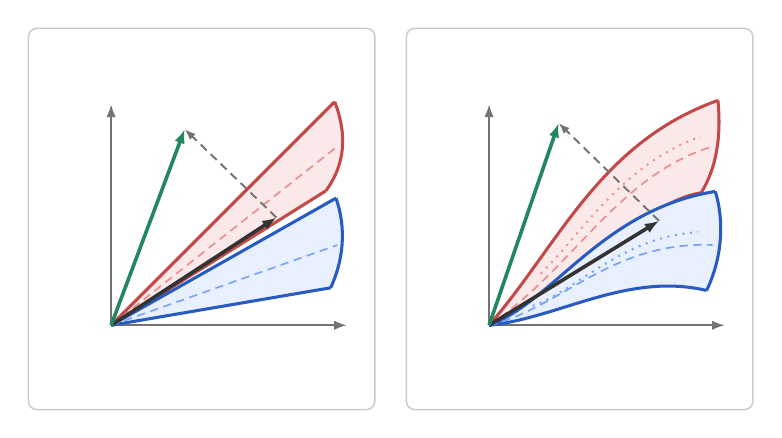
\begin{tikzpicture}
    \ifdefined\ONLYB
        \panelB
    \else
        \ifdefined\ONLYC
            \panelC
        \else
            \panelB
            \begin{scope}[xshift=4.80cm]
                \panelC
            \end{scope}
        \fi
    \fi
\end{tikzpicture}
\end{document}
'
% ---------------------------------------------------------------------------
\documentclass[tikz,border=2pt]{standalone}

\usepackage{tikz}
\usetikzlibrary{arrows.meta,positioning,calc}

\definecolor{pvoBlue}{HTML}{2F6FED}
\definecolor{pvoGreen}{HTML}{2AA876}
\definecolor{pvoRed}{HTML}{E05252}

\tikzset{
    line join=round, line cap=round,
    panel/.style={rounded corners=3pt, draw=black!20, line width=0.55pt},
    axis/.style={-{Latex[length=1.6mm]}, line width=0.7pt, draw=black!55},
    riskone/.style={line width=1.1pt, draw=pvoRed!88!black},
    risktwo/.style={line width=1.1pt, draw=pvoBlue!82!black},
    meanline/.style={line width=0.62pt, densely dashed},
    candidate/.style={-{Latex[length=1.8mm]}, line width=1.3pt, draw=black!80},
    accepted/.style={-{Latex[length=1.8mm]}, line width=1.3pt, draw=pvoGreen!80!black},
    correction/.style={-{Latex[length=1.4mm]}, line width=0.7pt, densely dashed, draw=black!55}
}

% --------------------------------------------------------------- panel (b) --
\newcommand{\panelB}{%
    \draw[panel] (-0.10,-0.12) rectangle (4.30,4.72);
    \begin{scope}[shift={(0.95,0.95)}, scale=0.85, shift={(-0.48,-0.52)}]
        \draw[axis] (0.48,0.52) -- (4.00,0.52);
        \draw[axis] (0.48,0.52) -- (0.48,3.82);

        % deterministic relative-velocity cone for obstacle 1
        \path[fill=pvoRed!13]
            (0.48,0.52) -- (3.82,3.86)
            .. controls (4.01,3.37) and (3.98,2.93) .. (3.69,2.53) -- cycle;
        \draw[riskone] (0.48,0.52) -- (3.82,3.86);
        \draw[riskone] (0.48,0.52) -- (3.69,2.53);
        \draw[riskone] (3.82,3.86) .. controls (4.01,3.37) and (3.98,2.93) .. (3.69,2.53);
        \draw[meanline, pvoRed!64] (0.48,0.52) -- (3.82,3.16);

        % deterministic relative-velocity cone for obstacle 2
        \path[fill=pvoBlue!11]
            (0.48,0.52) -- (3.84,2.42)
            .. controls (4.00,1.96) and (3.95,1.49) .. (3.76,1.08) -- cycle;
        \draw[risktwo] (0.48,0.52) -- (3.84,2.42);
        \draw[risktwo] (0.48,0.52) -- (3.76,1.08);
        \draw[risktwo] (3.84,2.42) .. controls (4.00,1.96) and (3.95,1.49) .. (3.76,1.08);
        \draw[meanline, pvoBlue!62] (0.48,0.52) -- (3.86,1.72);

        % candidate velocity / filtered velocity / correction
        \draw[candidate] (0.48,0.52) -- (2.95,2.13);
        \draw[accepted] (0.48,0.52) -- (1.58,3.45);
        \draw[correction] (2.95,2.13) -- (1.58,3.45);
    \end{scope}%
}

% --------------------------------------------------------------- panel (c) --
\newcommand{\panelC}{%
    \draw[panel] (-0.10,-0.12) rectangle (4.30,4.72);
    \begin{scope}[shift={(0.95,0.95)}, scale=0.85, shift={(-0.48,-0.52)}]
        \draw[axis] (0.48,0.52) -- (4.00,0.52);
        \draw[axis] (0.48,0.52) -- (0.48,3.82);

        % action-conditioned risk tube for obstacle 1
        \path[fill=pvoRed!13]
            (0.48,0.52)
            .. controls (1.52,1.72) and (2.13,3.25) .. (3.90,3.88)
            .. controls (3.95,3.33) and (3.88,2.88) .. (3.65,2.50)
            .. controls (2.72,2.35) and (1.64,1.02) .. (0.48,0.52) -- cycle;
        \draw[riskone]
            (0.48,0.52) .. controls (1.52,1.72) and (2.13,3.25) .. (3.90,3.88);
        \draw[riskone]
            (0.48,0.52) .. controls (1.64,1.02) and (2.72,2.35) .. (3.65,2.50);
        \draw[riskone] (3.90,3.88) .. controls (3.95,3.33) and (3.88,2.88) .. (3.65,2.50);
        \draw[meanline, pvoRed!65]
            (0.48,0.52) .. controls (1.72,1.35) and (2.38,2.73) .. (3.78,3.18);
        \draw[dotted, line width=0.75pt, pvoRed!62]
            (1.25,1.29) .. controls (1.86,1.88) and (2.46,2.92) .. (3.64,3.34);

        % action-conditioned risk tube for obstacle 2
        \path[fill=pvoBlue!11]
            (0.48,0.52)
            .. controls (1.45,0.88) and (2.17,2.25) .. (3.86,2.52)
            .. controls (4.00,2.06) and (3.96,1.52) .. (3.73,1.04)
            .. controls (2.55,1.32) and (1.53,0.63) .. (0.48,0.52) -- cycle;
        \draw[risktwo]
            (0.48,0.52) .. controls (1.45,0.88) and (2.17,2.25) .. (3.86,2.52);
        \draw[risktwo]
            (0.48,0.52) .. controls (1.53,0.63) and (2.55,1.32) .. (3.73,1.04);
        \draw[risktwo] (3.86,2.52) .. controls (4.00,2.06) and (3.96,1.52) .. (3.73,1.04);
        \draw[meanline, pvoBlue!64]
            (0.48,0.52) .. controls (1.55,0.77) and (2.30,1.78) .. (3.82,1.72);
        \draw[dotted, line width=0.75pt, pvoBlue!62]
            (1.13,0.81) .. controls (1.79,1.04) and (2.48,1.85) .. (3.60,1.91);

        % candidate velocity / filtered velocity / correction
        \draw[candidate] (0.48,0.52) -- (3.02,2.08);
        \draw[accepted] (0.48,0.52) -- (1.52,3.54);
        \draw[correction] (3.02,2.08) -- (1.52,3.54);
    \end{scope}%
}

\begin{document}
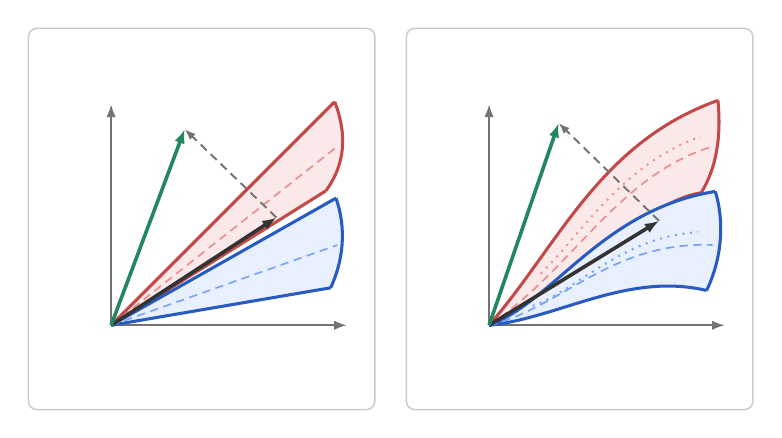
\begin{tikzpicture}
    \ifdefined\ONLYB
        \panelB
    \else
        \ifdefined\ONLYC
            \panelC
        \else
            \panelB
            \begin{scope}[xshift=4.80cm]
                \panelC
            \end{scope}
        \fi
    \fi
\end{tikzpicture}
\end{document}
'
% ---------------------------------------------------------------------------
\documentclass[tikz,border=2pt]{standalone}

\usepackage{tikz}
\usetikzlibrary{arrows.meta,positioning,calc}

\definecolor{pvoBlue}{HTML}{2F6FED}
\definecolor{pvoGreen}{HTML}{2AA876}
\definecolor{pvoRed}{HTML}{E05252}

\tikzset{
    line join=round, line cap=round,
    panel/.style={rounded corners=3pt, draw=black!20, line width=0.55pt},
    axis/.style={-{Latex[length=1.6mm]}, line width=0.7pt, draw=black!55},
    riskone/.style={line width=1.1pt, draw=pvoRed!88!black},
    risktwo/.style={line width=1.1pt, draw=pvoBlue!82!black},
    meanline/.style={line width=0.62pt, densely dashed},
    candidate/.style={-{Latex[length=1.8mm]}, line width=1.3pt, draw=black!80},
    accepted/.style={-{Latex[length=1.8mm]}, line width=1.3pt, draw=pvoGreen!80!black},
    correction/.style={-{Latex[length=1.4mm]}, line width=0.7pt, densely dashed, draw=black!55}
}

% --------------------------------------------------------------- panel (b) --
\newcommand{\panelB}{%
    \draw[panel] (-0.10,-0.12) rectangle (4.30,4.72);
    \begin{scope}[shift={(0.95,0.95)}, scale=0.85, shift={(-0.48,-0.52)}]
        \draw[axis] (0.48,0.52) -- (4.00,0.52);
        \draw[axis] (0.48,0.52) -- (0.48,3.82);

        % deterministic relative-velocity cone for obstacle 1
        \path[fill=pvoRed!13]
            (0.48,0.52) -- (3.82,3.86)
            .. controls (4.01,3.37) and (3.98,2.93) .. (3.69,2.53) -- cycle;
        \draw[riskone] (0.48,0.52) -- (3.82,3.86);
        \draw[riskone] (0.48,0.52) -- (3.69,2.53);
        \draw[riskone] (3.82,3.86) .. controls (4.01,3.37) and (3.98,2.93) .. (3.69,2.53);
        \draw[meanline, pvoRed!64] (0.48,0.52) -- (3.82,3.16);

        % deterministic relative-velocity cone for obstacle 2
        \path[fill=pvoBlue!11]
            (0.48,0.52) -- (3.84,2.42)
            .. controls (4.00,1.96) and (3.95,1.49) .. (3.76,1.08) -- cycle;
        \draw[risktwo] (0.48,0.52) -- (3.84,2.42);
        \draw[risktwo] (0.48,0.52) -- (3.76,1.08);
        \draw[risktwo] (3.84,2.42) .. controls (4.00,1.96) and (3.95,1.49) .. (3.76,1.08);
        \draw[meanline, pvoBlue!62] (0.48,0.52) -- (3.86,1.72);

        % candidate velocity / filtered velocity / correction
        \draw[candidate] (0.48,0.52) -- (2.95,2.13);
        \draw[accepted] (0.48,0.52) -- (1.58,3.45);
        \draw[correction] (2.95,2.13) -- (1.58,3.45);
    \end{scope}%
}

% --------------------------------------------------------------- panel (c) --
\newcommand{\panelC}{%
    \draw[panel] (-0.10,-0.12) rectangle (4.30,4.72);
    \begin{scope}[shift={(0.95,0.95)}, scale=0.85, shift={(-0.48,-0.52)}]
        \draw[axis] (0.48,0.52) -- (4.00,0.52);
        \draw[axis] (0.48,0.52) -- (0.48,3.82);

        % action-conditioned risk tube for obstacle 1
        \path[fill=pvoRed!13]
            (0.48,0.52)
            .. controls (1.52,1.72) and (2.13,3.25) .. (3.90,3.88)
            .. controls (3.95,3.33) and (3.88,2.88) .. (3.65,2.50)
            .. controls (2.72,2.35) and (1.64,1.02) .. (0.48,0.52) -- cycle;
        \draw[riskone]
            (0.48,0.52) .. controls (1.52,1.72) and (2.13,3.25) .. (3.90,3.88);
        \draw[riskone]
            (0.48,0.52) .. controls (1.64,1.02) and (2.72,2.35) .. (3.65,2.50);
        \draw[riskone] (3.90,3.88) .. controls (3.95,3.33) and (3.88,2.88) .. (3.65,2.50);
        \draw[meanline, pvoRed!65]
            (0.48,0.52) .. controls (1.72,1.35) and (2.38,2.73) .. (3.78,3.18);
        \draw[dotted, line width=0.75pt, pvoRed!62]
            (1.25,1.29) .. controls (1.86,1.88) and (2.46,2.92) .. (3.64,3.34);

        % action-conditioned risk tube for obstacle 2
        \path[fill=pvoBlue!11]
            (0.48,0.52)
            .. controls (1.45,0.88) and (2.17,2.25) .. (3.86,2.52)
            .. controls (4.00,2.06) and (3.96,1.52) .. (3.73,1.04)
            .. controls (2.55,1.32) and (1.53,0.63) .. (0.48,0.52) -- cycle;
        \draw[risktwo]
            (0.48,0.52) .. controls (1.45,0.88) and (2.17,2.25) .. (3.86,2.52);
        \draw[risktwo]
            (0.48,0.52) .. controls (1.53,0.63) and (2.55,1.32) .. (3.73,1.04);
        \draw[risktwo] (3.86,2.52) .. controls (4.00,2.06) and (3.96,1.52) .. (3.73,1.04);
        \draw[meanline, pvoBlue!64]
            (0.48,0.52) .. controls (1.55,0.77) and (2.30,1.78) .. (3.82,1.72);
        \draw[dotted, line width=0.75pt, pvoBlue!62]
            (1.13,0.81) .. controls (1.79,1.04) and (2.48,1.85) .. (3.60,1.91);

        % candidate velocity / filtered velocity / correction
        \draw[candidate] (0.48,0.52) -- (3.02,2.08);
        \draw[accepted] (0.48,0.52) -- (1.52,3.54);
        \draw[correction] (3.02,2.08) -- (1.52,3.54);
    \end{scope}%
}

\begin{document}
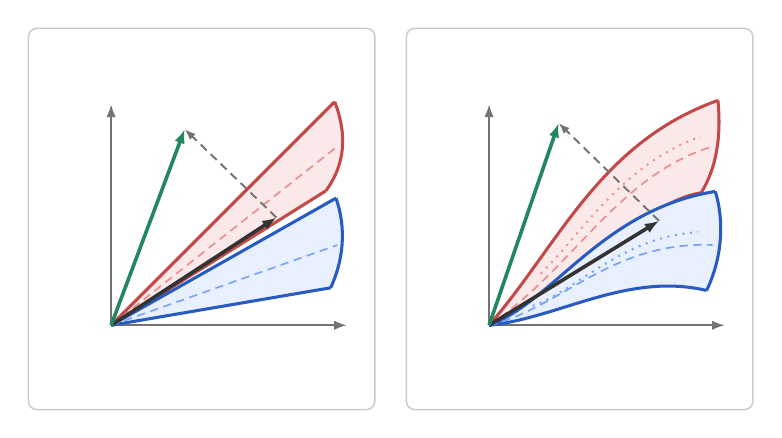
\begin{tikzpicture}
    \ifdefined\ONLYB
        \panelB
    \else
        \ifdefined\ONLYC
            \panelC
        \else
            \panelB
            \begin{scope}[xshift=4.80cm]
                \panelC
            \end{scope}
        \fi
    \fi
\end{tikzpicture}
\end{document}
'
%    xelatex -jobname=fig1_bc_clean '% ---------------------------------------------------------------------------
%  Figure 1 panels (b) and (c) -- TEXT-FREE export for PowerPoint.
%
%  Every label / annotation has been removed (panel titles, axis labels,
%  "$v_t^{cand}$", "$R_{1,\eta}$", "$VO^T_1$", origin "0", correction symbols,
%  the union equations ...).  Geometry, colours and line weights are identical
%  to the in-paper TikZ figure, so text can be re-added by hand in PPT.
%
%  Build from this folder:
%    xelatex -jobname=fig1_b_clean  '\def\ONLYB{}% ---------------------------------------------------------------------------
%  Figure 1 panels (b) and (c) -- TEXT-FREE export for PowerPoint.
%
%  Every label / annotation has been removed (panel titles, axis labels,
%  "$v_t^{cand}$", "$R_{1,\eta}$", "$VO^T_1$", origin "0", correction symbols,
%  the union equations ...).  Geometry, colours and line weights are identical
%  to the in-paper TikZ figure, so text can be re-added by hand in PPT.
%
%  Build from this folder:
%    xelatex -jobname=fig1_b_clean  '\def\ONLYB{}% ---------------------------------------------------------------------------
%  Figure 1 panels (b) and (c) -- TEXT-FREE export for PowerPoint.
%
%  Every label / annotation has been removed (panel titles, axis labels,
%  "$v_t^{cand}$", "$R_{1,\eta}$", "$VO^T_1$", origin "0", correction symbols,
%  the union equations ...).  Geometry, colours and line weights are identical
%  to the in-paper TikZ figure, so text can be re-added by hand in PPT.
%
%  Build from this folder:
%    xelatex -jobname=fig1_b_clean  '\def\ONLYB{}\input{fig1_bc_clean.tex}'
%    xelatex -jobname=fig1_c_clean  '\def\ONLYC{}\input{fig1_bc_clean.tex}'
%    xelatex -jobname=fig1_bc_clean '\input{fig1_bc_clean.tex}'
% ---------------------------------------------------------------------------
\documentclass[tikz,border=2pt]{standalone}

\usepackage{tikz}
\usetikzlibrary{arrows.meta,positioning,calc}

\definecolor{pvoBlue}{HTML}{2F6FED}
\definecolor{pvoGreen}{HTML}{2AA876}
\definecolor{pvoRed}{HTML}{E05252}

\tikzset{
    line join=round, line cap=round,
    panel/.style={rounded corners=3pt, draw=black!20, line width=0.55pt},
    axis/.style={-{Latex[length=1.6mm]}, line width=0.7pt, draw=black!55},
    riskone/.style={line width=1.1pt, draw=pvoRed!88!black},
    risktwo/.style={line width=1.1pt, draw=pvoBlue!82!black},
    meanline/.style={line width=0.62pt, densely dashed},
    candidate/.style={-{Latex[length=1.8mm]}, line width=1.3pt, draw=black!80},
    accepted/.style={-{Latex[length=1.8mm]}, line width=1.3pt, draw=pvoGreen!80!black},
    correction/.style={-{Latex[length=1.4mm]}, line width=0.7pt, densely dashed, draw=black!55}
}

% --------------------------------------------------------------- panel (b) --
\newcommand{\panelB}{%
    \draw[panel] (-0.10,-0.12) rectangle (4.30,4.72);
    \begin{scope}[shift={(0.95,0.95)}, scale=0.85, shift={(-0.48,-0.52)}]
        \draw[axis] (0.48,0.52) -- (4.00,0.52);
        \draw[axis] (0.48,0.52) -- (0.48,3.82);

        % deterministic relative-velocity cone for obstacle 1
        \path[fill=pvoRed!13]
            (0.48,0.52) -- (3.82,3.86)
            .. controls (4.01,3.37) and (3.98,2.93) .. (3.69,2.53) -- cycle;
        \draw[riskone] (0.48,0.52) -- (3.82,3.86);
        \draw[riskone] (0.48,0.52) -- (3.69,2.53);
        \draw[riskone] (3.82,3.86) .. controls (4.01,3.37) and (3.98,2.93) .. (3.69,2.53);
        \draw[meanline, pvoRed!64] (0.48,0.52) -- (3.82,3.16);

        % deterministic relative-velocity cone for obstacle 2
        \path[fill=pvoBlue!11]
            (0.48,0.52) -- (3.84,2.42)
            .. controls (4.00,1.96) and (3.95,1.49) .. (3.76,1.08) -- cycle;
        \draw[risktwo] (0.48,0.52) -- (3.84,2.42);
        \draw[risktwo] (0.48,0.52) -- (3.76,1.08);
        \draw[risktwo] (3.84,2.42) .. controls (4.00,1.96) and (3.95,1.49) .. (3.76,1.08);
        \draw[meanline, pvoBlue!62] (0.48,0.52) -- (3.86,1.72);

        % candidate velocity / filtered velocity / correction
        \draw[candidate] (0.48,0.52) -- (2.95,2.13);
        \draw[accepted] (0.48,0.52) -- (1.58,3.45);
        \draw[correction] (2.95,2.13) -- (1.58,3.45);
    \end{scope}%
}

% --------------------------------------------------------------- panel (c) --
\newcommand{\panelC}{%
    \draw[panel] (-0.10,-0.12) rectangle (4.30,4.72);
    \begin{scope}[shift={(0.95,0.95)}, scale=0.85, shift={(-0.48,-0.52)}]
        \draw[axis] (0.48,0.52) -- (4.00,0.52);
        \draw[axis] (0.48,0.52) -- (0.48,3.82);

        % action-conditioned risk tube for obstacle 1
        \path[fill=pvoRed!13]
            (0.48,0.52)
            .. controls (1.52,1.72) and (2.13,3.25) .. (3.90,3.88)
            .. controls (3.95,3.33) and (3.88,2.88) .. (3.65,2.50)
            .. controls (2.72,2.35) and (1.64,1.02) .. (0.48,0.52) -- cycle;
        \draw[riskone]
            (0.48,0.52) .. controls (1.52,1.72) and (2.13,3.25) .. (3.90,3.88);
        \draw[riskone]
            (0.48,0.52) .. controls (1.64,1.02) and (2.72,2.35) .. (3.65,2.50);
        \draw[riskone] (3.90,3.88) .. controls (3.95,3.33) and (3.88,2.88) .. (3.65,2.50);
        \draw[meanline, pvoRed!65]
            (0.48,0.52) .. controls (1.72,1.35) and (2.38,2.73) .. (3.78,3.18);
        \draw[dotted, line width=0.75pt, pvoRed!62]
            (1.25,1.29) .. controls (1.86,1.88) and (2.46,2.92) .. (3.64,3.34);

        % action-conditioned risk tube for obstacle 2
        \path[fill=pvoBlue!11]
            (0.48,0.52)
            .. controls (1.45,0.88) and (2.17,2.25) .. (3.86,2.52)
            .. controls (4.00,2.06) and (3.96,1.52) .. (3.73,1.04)
            .. controls (2.55,1.32) and (1.53,0.63) .. (0.48,0.52) -- cycle;
        \draw[risktwo]
            (0.48,0.52) .. controls (1.45,0.88) and (2.17,2.25) .. (3.86,2.52);
        \draw[risktwo]
            (0.48,0.52) .. controls (1.53,0.63) and (2.55,1.32) .. (3.73,1.04);
        \draw[risktwo] (3.86,2.52) .. controls (4.00,2.06) and (3.96,1.52) .. (3.73,1.04);
        \draw[meanline, pvoBlue!64]
            (0.48,0.52) .. controls (1.55,0.77) and (2.30,1.78) .. (3.82,1.72);
        \draw[dotted, line width=0.75pt, pvoBlue!62]
            (1.13,0.81) .. controls (1.79,1.04) and (2.48,1.85) .. (3.60,1.91);

        % candidate velocity / filtered velocity / correction
        \draw[candidate] (0.48,0.52) -- (3.02,2.08);
        \draw[accepted] (0.48,0.52) -- (1.52,3.54);
        \draw[correction] (3.02,2.08) -- (1.52,3.54);
    \end{scope}%
}

\begin{document}
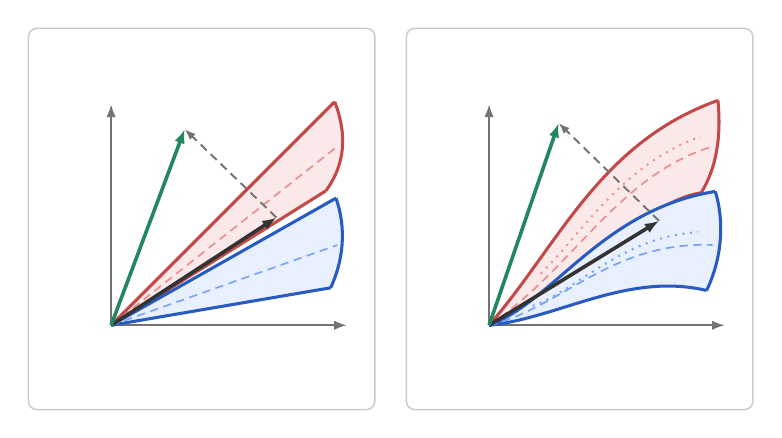
\begin{tikzpicture}
    \ifdefined\ONLYB
        \panelB
    \else
        \ifdefined\ONLYC
            \panelC
        \else
            \panelB
            \begin{scope}[xshift=4.80cm]
                \panelC
            \end{scope}
        \fi
    \fi
\end{tikzpicture}
\end{document}
'
%    xelatex -jobname=fig1_c_clean  '\def\ONLYC{}% ---------------------------------------------------------------------------
%  Figure 1 panels (b) and (c) -- TEXT-FREE export for PowerPoint.
%
%  Every label / annotation has been removed (panel titles, axis labels,
%  "$v_t^{cand}$", "$R_{1,\eta}$", "$VO^T_1$", origin "0", correction symbols,
%  the union equations ...).  Geometry, colours and line weights are identical
%  to the in-paper TikZ figure, so text can be re-added by hand in PPT.
%
%  Build from this folder:
%    xelatex -jobname=fig1_b_clean  '\def\ONLYB{}\input{fig1_bc_clean.tex}'
%    xelatex -jobname=fig1_c_clean  '\def\ONLYC{}\input{fig1_bc_clean.tex}'
%    xelatex -jobname=fig1_bc_clean '\input{fig1_bc_clean.tex}'
% ---------------------------------------------------------------------------
\documentclass[tikz,border=2pt]{standalone}

\usepackage{tikz}
\usetikzlibrary{arrows.meta,positioning,calc}

\definecolor{pvoBlue}{HTML}{2F6FED}
\definecolor{pvoGreen}{HTML}{2AA876}
\definecolor{pvoRed}{HTML}{E05252}

\tikzset{
    line join=round, line cap=round,
    panel/.style={rounded corners=3pt, draw=black!20, line width=0.55pt},
    axis/.style={-{Latex[length=1.6mm]}, line width=0.7pt, draw=black!55},
    riskone/.style={line width=1.1pt, draw=pvoRed!88!black},
    risktwo/.style={line width=1.1pt, draw=pvoBlue!82!black},
    meanline/.style={line width=0.62pt, densely dashed},
    candidate/.style={-{Latex[length=1.8mm]}, line width=1.3pt, draw=black!80},
    accepted/.style={-{Latex[length=1.8mm]}, line width=1.3pt, draw=pvoGreen!80!black},
    correction/.style={-{Latex[length=1.4mm]}, line width=0.7pt, densely dashed, draw=black!55}
}

% --------------------------------------------------------------- panel (b) --
\newcommand{\panelB}{%
    \draw[panel] (-0.10,-0.12) rectangle (4.30,4.72);
    \begin{scope}[shift={(0.95,0.95)}, scale=0.85, shift={(-0.48,-0.52)}]
        \draw[axis] (0.48,0.52) -- (4.00,0.52);
        \draw[axis] (0.48,0.52) -- (0.48,3.82);

        % deterministic relative-velocity cone for obstacle 1
        \path[fill=pvoRed!13]
            (0.48,0.52) -- (3.82,3.86)
            .. controls (4.01,3.37) and (3.98,2.93) .. (3.69,2.53) -- cycle;
        \draw[riskone] (0.48,0.52) -- (3.82,3.86);
        \draw[riskone] (0.48,0.52) -- (3.69,2.53);
        \draw[riskone] (3.82,3.86) .. controls (4.01,3.37) and (3.98,2.93) .. (3.69,2.53);
        \draw[meanline, pvoRed!64] (0.48,0.52) -- (3.82,3.16);

        % deterministic relative-velocity cone for obstacle 2
        \path[fill=pvoBlue!11]
            (0.48,0.52) -- (3.84,2.42)
            .. controls (4.00,1.96) and (3.95,1.49) .. (3.76,1.08) -- cycle;
        \draw[risktwo] (0.48,0.52) -- (3.84,2.42);
        \draw[risktwo] (0.48,0.52) -- (3.76,1.08);
        \draw[risktwo] (3.84,2.42) .. controls (4.00,1.96) and (3.95,1.49) .. (3.76,1.08);
        \draw[meanline, pvoBlue!62] (0.48,0.52) -- (3.86,1.72);

        % candidate velocity / filtered velocity / correction
        \draw[candidate] (0.48,0.52) -- (2.95,2.13);
        \draw[accepted] (0.48,0.52) -- (1.58,3.45);
        \draw[correction] (2.95,2.13) -- (1.58,3.45);
    \end{scope}%
}

% --------------------------------------------------------------- panel (c) --
\newcommand{\panelC}{%
    \draw[panel] (-0.10,-0.12) rectangle (4.30,4.72);
    \begin{scope}[shift={(0.95,0.95)}, scale=0.85, shift={(-0.48,-0.52)}]
        \draw[axis] (0.48,0.52) -- (4.00,0.52);
        \draw[axis] (0.48,0.52) -- (0.48,3.82);

        % action-conditioned risk tube for obstacle 1
        \path[fill=pvoRed!13]
            (0.48,0.52)
            .. controls (1.52,1.72) and (2.13,3.25) .. (3.90,3.88)
            .. controls (3.95,3.33) and (3.88,2.88) .. (3.65,2.50)
            .. controls (2.72,2.35) and (1.64,1.02) .. (0.48,0.52) -- cycle;
        \draw[riskone]
            (0.48,0.52) .. controls (1.52,1.72) and (2.13,3.25) .. (3.90,3.88);
        \draw[riskone]
            (0.48,0.52) .. controls (1.64,1.02) and (2.72,2.35) .. (3.65,2.50);
        \draw[riskone] (3.90,3.88) .. controls (3.95,3.33) and (3.88,2.88) .. (3.65,2.50);
        \draw[meanline, pvoRed!65]
            (0.48,0.52) .. controls (1.72,1.35) and (2.38,2.73) .. (3.78,3.18);
        \draw[dotted, line width=0.75pt, pvoRed!62]
            (1.25,1.29) .. controls (1.86,1.88) and (2.46,2.92) .. (3.64,3.34);

        % action-conditioned risk tube for obstacle 2
        \path[fill=pvoBlue!11]
            (0.48,0.52)
            .. controls (1.45,0.88) and (2.17,2.25) .. (3.86,2.52)
            .. controls (4.00,2.06) and (3.96,1.52) .. (3.73,1.04)
            .. controls (2.55,1.32) and (1.53,0.63) .. (0.48,0.52) -- cycle;
        \draw[risktwo]
            (0.48,0.52) .. controls (1.45,0.88) and (2.17,2.25) .. (3.86,2.52);
        \draw[risktwo]
            (0.48,0.52) .. controls (1.53,0.63) and (2.55,1.32) .. (3.73,1.04);
        \draw[risktwo] (3.86,2.52) .. controls (4.00,2.06) and (3.96,1.52) .. (3.73,1.04);
        \draw[meanline, pvoBlue!64]
            (0.48,0.52) .. controls (1.55,0.77) and (2.30,1.78) .. (3.82,1.72);
        \draw[dotted, line width=0.75pt, pvoBlue!62]
            (1.13,0.81) .. controls (1.79,1.04) and (2.48,1.85) .. (3.60,1.91);

        % candidate velocity / filtered velocity / correction
        \draw[candidate] (0.48,0.52) -- (3.02,2.08);
        \draw[accepted] (0.48,0.52) -- (1.52,3.54);
        \draw[correction] (3.02,2.08) -- (1.52,3.54);
    \end{scope}%
}

\begin{document}
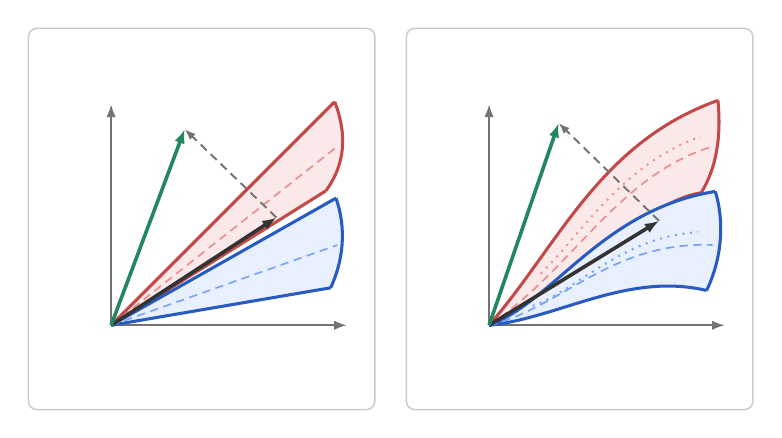
\begin{tikzpicture}
    \ifdefined\ONLYB
        \panelB
    \else
        \ifdefined\ONLYC
            \panelC
        \else
            \panelB
            \begin{scope}[xshift=4.80cm]
                \panelC
            \end{scope}
        \fi
    \fi
\end{tikzpicture}
\end{document}
'
%    xelatex -jobname=fig1_bc_clean '% ---------------------------------------------------------------------------
%  Figure 1 panels (b) and (c) -- TEXT-FREE export for PowerPoint.
%
%  Every label / annotation has been removed (panel titles, axis labels,
%  "$v_t^{cand}$", "$R_{1,\eta}$", "$VO^T_1$", origin "0", correction symbols,
%  the union equations ...).  Geometry, colours and line weights are identical
%  to the in-paper TikZ figure, so text can be re-added by hand in PPT.
%
%  Build from this folder:
%    xelatex -jobname=fig1_b_clean  '\def\ONLYB{}\input{fig1_bc_clean.tex}'
%    xelatex -jobname=fig1_c_clean  '\def\ONLYC{}\input{fig1_bc_clean.tex}'
%    xelatex -jobname=fig1_bc_clean '\input{fig1_bc_clean.tex}'
% ---------------------------------------------------------------------------
\documentclass[tikz,border=2pt]{standalone}

\usepackage{tikz}
\usetikzlibrary{arrows.meta,positioning,calc}

\definecolor{pvoBlue}{HTML}{2F6FED}
\definecolor{pvoGreen}{HTML}{2AA876}
\definecolor{pvoRed}{HTML}{E05252}

\tikzset{
    line join=round, line cap=round,
    panel/.style={rounded corners=3pt, draw=black!20, line width=0.55pt},
    axis/.style={-{Latex[length=1.6mm]}, line width=0.7pt, draw=black!55},
    riskone/.style={line width=1.1pt, draw=pvoRed!88!black},
    risktwo/.style={line width=1.1pt, draw=pvoBlue!82!black},
    meanline/.style={line width=0.62pt, densely dashed},
    candidate/.style={-{Latex[length=1.8mm]}, line width=1.3pt, draw=black!80},
    accepted/.style={-{Latex[length=1.8mm]}, line width=1.3pt, draw=pvoGreen!80!black},
    correction/.style={-{Latex[length=1.4mm]}, line width=0.7pt, densely dashed, draw=black!55}
}

% --------------------------------------------------------------- panel (b) --
\newcommand{\panelB}{%
    \draw[panel] (-0.10,-0.12) rectangle (4.30,4.72);
    \begin{scope}[shift={(0.95,0.95)}, scale=0.85, shift={(-0.48,-0.52)}]
        \draw[axis] (0.48,0.52) -- (4.00,0.52);
        \draw[axis] (0.48,0.52) -- (0.48,3.82);

        % deterministic relative-velocity cone for obstacle 1
        \path[fill=pvoRed!13]
            (0.48,0.52) -- (3.82,3.86)
            .. controls (4.01,3.37) and (3.98,2.93) .. (3.69,2.53) -- cycle;
        \draw[riskone] (0.48,0.52) -- (3.82,3.86);
        \draw[riskone] (0.48,0.52) -- (3.69,2.53);
        \draw[riskone] (3.82,3.86) .. controls (4.01,3.37) and (3.98,2.93) .. (3.69,2.53);
        \draw[meanline, pvoRed!64] (0.48,0.52) -- (3.82,3.16);

        % deterministic relative-velocity cone for obstacle 2
        \path[fill=pvoBlue!11]
            (0.48,0.52) -- (3.84,2.42)
            .. controls (4.00,1.96) and (3.95,1.49) .. (3.76,1.08) -- cycle;
        \draw[risktwo] (0.48,0.52) -- (3.84,2.42);
        \draw[risktwo] (0.48,0.52) -- (3.76,1.08);
        \draw[risktwo] (3.84,2.42) .. controls (4.00,1.96) and (3.95,1.49) .. (3.76,1.08);
        \draw[meanline, pvoBlue!62] (0.48,0.52) -- (3.86,1.72);

        % candidate velocity / filtered velocity / correction
        \draw[candidate] (0.48,0.52) -- (2.95,2.13);
        \draw[accepted] (0.48,0.52) -- (1.58,3.45);
        \draw[correction] (2.95,2.13) -- (1.58,3.45);
    \end{scope}%
}

% --------------------------------------------------------------- panel (c) --
\newcommand{\panelC}{%
    \draw[panel] (-0.10,-0.12) rectangle (4.30,4.72);
    \begin{scope}[shift={(0.95,0.95)}, scale=0.85, shift={(-0.48,-0.52)}]
        \draw[axis] (0.48,0.52) -- (4.00,0.52);
        \draw[axis] (0.48,0.52) -- (0.48,3.82);

        % action-conditioned risk tube for obstacle 1
        \path[fill=pvoRed!13]
            (0.48,0.52)
            .. controls (1.52,1.72) and (2.13,3.25) .. (3.90,3.88)
            .. controls (3.95,3.33) and (3.88,2.88) .. (3.65,2.50)
            .. controls (2.72,2.35) and (1.64,1.02) .. (0.48,0.52) -- cycle;
        \draw[riskone]
            (0.48,0.52) .. controls (1.52,1.72) and (2.13,3.25) .. (3.90,3.88);
        \draw[riskone]
            (0.48,0.52) .. controls (1.64,1.02) and (2.72,2.35) .. (3.65,2.50);
        \draw[riskone] (3.90,3.88) .. controls (3.95,3.33) and (3.88,2.88) .. (3.65,2.50);
        \draw[meanline, pvoRed!65]
            (0.48,0.52) .. controls (1.72,1.35) and (2.38,2.73) .. (3.78,3.18);
        \draw[dotted, line width=0.75pt, pvoRed!62]
            (1.25,1.29) .. controls (1.86,1.88) and (2.46,2.92) .. (3.64,3.34);

        % action-conditioned risk tube for obstacle 2
        \path[fill=pvoBlue!11]
            (0.48,0.52)
            .. controls (1.45,0.88) and (2.17,2.25) .. (3.86,2.52)
            .. controls (4.00,2.06) and (3.96,1.52) .. (3.73,1.04)
            .. controls (2.55,1.32) and (1.53,0.63) .. (0.48,0.52) -- cycle;
        \draw[risktwo]
            (0.48,0.52) .. controls (1.45,0.88) and (2.17,2.25) .. (3.86,2.52);
        \draw[risktwo]
            (0.48,0.52) .. controls (1.53,0.63) and (2.55,1.32) .. (3.73,1.04);
        \draw[risktwo] (3.86,2.52) .. controls (4.00,2.06) and (3.96,1.52) .. (3.73,1.04);
        \draw[meanline, pvoBlue!64]
            (0.48,0.52) .. controls (1.55,0.77) and (2.30,1.78) .. (3.82,1.72);
        \draw[dotted, line width=0.75pt, pvoBlue!62]
            (1.13,0.81) .. controls (1.79,1.04) and (2.48,1.85) .. (3.60,1.91);

        % candidate velocity / filtered velocity / correction
        \draw[candidate] (0.48,0.52) -- (3.02,2.08);
        \draw[accepted] (0.48,0.52) -- (1.52,3.54);
        \draw[correction] (3.02,2.08) -- (1.52,3.54);
    \end{scope}%
}

\begin{document}
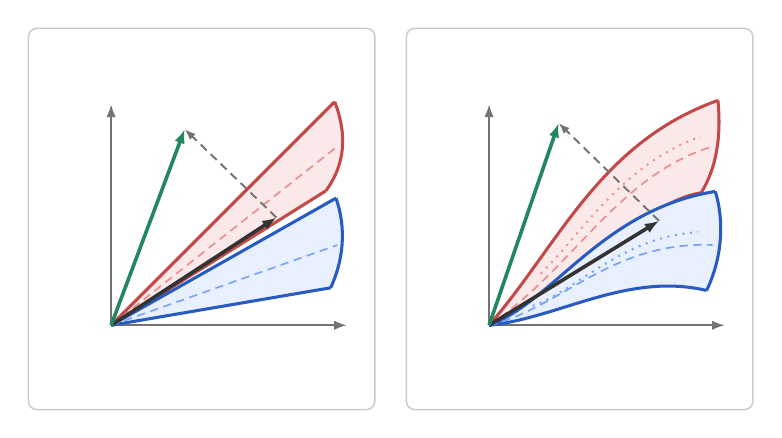
\begin{tikzpicture}
    \ifdefined\ONLYB
        \panelB
    \else
        \ifdefined\ONLYC
            \panelC
        \else
            \panelB
            \begin{scope}[xshift=4.80cm]
                \panelC
            \end{scope}
        \fi
    \fi
\end{tikzpicture}
\end{document}
'
% ---------------------------------------------------------------------------
\documentclass[tikz,border=2pt]{standalone}

\usepackage{tikz}
\usetikzlibrary{arrows.meta,positioning,calc}

\definecolor{pvoBlue}{HTML}{2F6FED}
\definecolor{pvoGreen}{HTML}{2AA876}
\definecolor{pvoRed}{HTML}{E05252}

\tikzset{
    line join=round, line cap=round,
    panel/.style={rounded corners=3pt, draw=black!20, line width=0.55pt},
    axis/.style={-{Latex[length=1.6mm]}, line width=0.7pt, draw=black!55},
    riskone/.style={line width=1.1pt, draw=pvoRed!88!black},
    risktwo/.style={line width=1.1pt, draw=pvoBlue!82!black},
    meanline/.style={line width=0.62pt, densely dashed},
    candidate/.style={-{Latex[length=1.8mm]}, line width=1.3pt, draw=black!80},
    accepted/.style={-{Latex[length=1.8mm]}, line width=1.3pt, draw=pvoGreen!80!black},
    correction/.style={-{Latex[length=1.4mm]}, line width=0.7pt, densely dashed, draw=black!55}
}

% --------------------------------------------------------------- panel (b) --
\newcommand{\panelB}{%
    \draw[panel] (-0.10,-0.12) rectangle (4.30,4.72);
    \begin{scope}[shift={(0.95,0.95)}, scale=0.85, shift={(-0.48,-0.52)}]
        \draw[axis] (0.48,0.52) -- (4.00,0.52);
        \draw[axis] (0.48,0.52) -- (0.48,3.82);

        % deterministic relative-velocity cone for obstacle 1
        \path[fill=pvoRed!13]
            (0.48,0.52) -- (3.82,3.86)
            .. controls (4.01,3.37) and (3.98,2.93) .. (3.69,2.53) -- cycle;
        \draw[riskone] (0.48,0.52) -- (3.82,3.86);
        \draw[riskone] (0.48,0.52) -- (3.69,2.53);
        \draw[riskone] (3.82,3.86) .. controls (4.01,3.37) and (3.98,2.93) .. (3.69,2.53);
        \draw[meanline, pvoRed!64] (0.48,0.52) -- (3.82,3.16);

        % deterministic relative-velocity cone for obstacle 2
        \path[fill=pvoBlue!11]
            (0.48,0.52) -- (3.84,2.42)
            .. controls (4.00,1.96) and (3.95,1.49) .. (3.76,1.08) -- cycle;
        \draw[risktwo] (0.48,0.52) -- (3.84,2.42);
        \draw[risktwo] (0.48,0.52) -- (3.76,1.08);
        \draw[risktwo] (3.84,2.42) .. controls (4.00,1.96) and (3.95,1.49) .. (3.76,1.08);
        \draw[meanline, pvoBlue!62] (0.48,0.52) -- (3.86,1.72);

        % candidate velocity / filtered velocity / correction
        \draw[candidate] (0.48,0.52) -- (2.95,2.13);
        \draw[accepted] (0.48,0.52) -- (1.58,3.45);
        \draw[correction] (2.95,2.13) -- (1.58,3.45);
    \end{scope}%
}

% --------------------------------------------------------------- panel (c) --
\newcommand{\panelC}{%
    \draw[panel] (-0.10,-0.12) rectangle (4.30,4.72);
    \begin{scope}[shift={(0.95,0.95)}, scale=0.85, shift={(-0.48,-0.52)}]
        \draw[axis] (0.48,0.52) -- (4.00,0.52);
        \draw[axis] (0.48,0.52) -- (0.48,3.82);

        % action-conditioned risk tube for obstacle 1
        \path[fill=pvoRed!13]
            (0.48,0.52)
            .. controls (1.52,1.72) and (2.13,3.25) .. (3.90,3.88)
            .. controls (3.95,3.33) and (3.88,2.88) .. (3.65,2.50)
            .. controls (2.72,2.35) and (1.64,1.02) .. (0.48,0.52) -- cycle;
        \draw[riskone]
            (0.48,0.52) .. controls (1.52,1.72) and (2.13,3.25) .. (3.90,3.88);
        \draw[riskone]
            (0.48,0.52) .. controls (1.64,1.02) and (2.72,2.35) .. (3.65,2.50);
        \draw[riskone] (3.90,3.88) .. controls (3.95,3.33) and (3.88,2.88) .. (3.65,2.50);
        \draw[meanline, pvoRed!65]
            (0.48,0.52) .. controls (1.72,1.35) and (2.38,2.73) .. (3.78,3.18);
        \draw[dotted, line width=0.75pt, pvoRed!62]
            (1.25,1.29) .. controls (1.86,1.88) and (2.46,2.92) .. (3.64,3.34);

        % action-conditioned risk tube for obstacle 2
        \path[fill=pvoBlue!11]
            (0.48,0.52)
            .. controls (1.45,0.88) and (2.17,2.25) .. (3.86,2.52)
            .. controls (4.00,2.06) and (3.96,1.52) .. (3.73,1.04)
            .. controls (2.55,1.32) and (1.53,0.63) .. (0.48,0.52) -- cycle;
        \draw[risktwo]
            (0.48,0.52) .. controls (1.45,0.88) and (2.17,2.25) .. (3.86,2.52);
        \draw[risktwo]
            (0.48,0.52) .. controls (1.53,0.63) and (2.55,1.32) .. (3.73,1.04);
        \draw[risktwo] (3.86,2.52) .. controls (4.00,2.06) and (3.96,1.52) .. (3.73,1.04);
        \draw[meanline, pvoBlue!64]
            (0.48,0.52) .. controls (1.55,0.77) and (2.30,1.78) .. (3.82,1.72);
        \draw[dotted, line width=0.75pt, pvoBlue!62]
            (1.13,0.81) .. controls (1.79,1.04) and (2.48,1.85) .. (3.60,1.91);

        % candidate velocity / filtered velocity / correction
        \draw[candidate] (0.48,0.52) -- (3.02,2.08);
        \draw[accepted] (0.48,0.52) -- (1.52,3.54);
        \draw[correction] (3.02,2.08) -- (1.52,3.54);
    \end{scope}%
}

\begin{document}
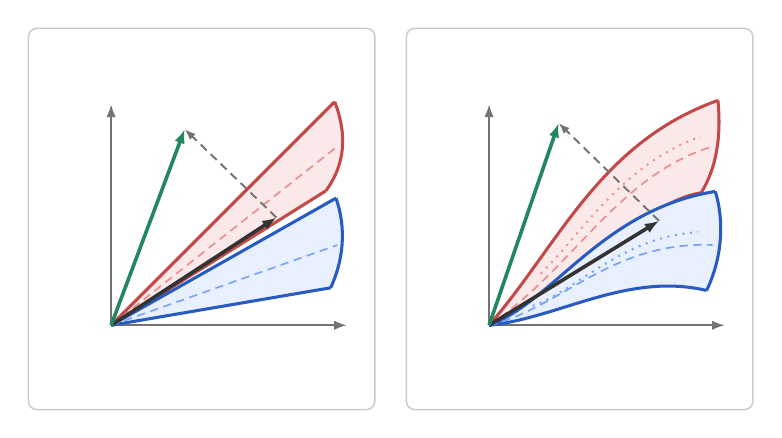
\begin{tikzpicture}
    \ifdefined\ONLYB
        \panelB
    \else
        \ifdefined\ONLYC
            \panelC
        \else
            \panelB
            \begin{scope}[xshift=4.80cm]
                \panelC
            \end{scope}
        \fi
    \fi
\end{tikzpicture}
\end{document}
'
%    xelatex -jobname=fig1_c_clean  '\def\ONLYC{}% ---------------------------------------------------------------------------
%  Figure 1 panels (b) and (c) -- TEXT-FREE export for PowerPoint.
%
%  Every label / annotation has been removed (panel titles, axis labels,
%  "$v_t^{cand}$", "$R_{1,\eta}$", "$VO^T_1$", origin "0", correction symbols,
%  the union equations ...).  Geometry, colours and line weights are identical
%  to the in-paper TikZ figure, so text can be re-added by hand in PPT.
%
%  Build from this folder:
%    xelatex -jobname=fig1_b_clean  '\def\ONLYB{}% ---------------------------------------------------------------------------
%  Figure 1 panels (b) and (c) -- TEXT-FREE export for PowerPoint.
%
%  Every label / annotation has been removed (panel titles, axis labels,
%  "$v_t^{cand}$", "$R_{1,\eta}$", "$VO^T_1$", origin "0", correction symbols,
%  the union equations ...).  Geometry, colours and line weights are identical
%  to the in-paper TikZ figure, so text can be re-added by hand in PPT.
%
%  Build from this folder:
%    xelatex -jobname=fig1_b_clean  '\def\ONLYB{}\input{fig1_bc_clean.tex}'
%    xelatex -jobname=fig1_c_clean  '\def\ONLYC{}\input{fig1_bc_clean.tex}'
%    xelatex -jobname=fig1_bc_clean '\input{fig1_bc_clean.tex}'
% ---------------------------------------------------------------------------
\documentclass[tikz,border=2pt]{standalone}

\usepackage{tikz}
\usetikzlibrary{arrows.meta,positioning,calc}

\definecolor{pvoBlue}{HTML}{2F6FED}
\definecolor{pvoGreen}{HTML}{2AA876}
\definecolor{pvoRed}{HTML}{E05252}

\tikzset{
    line join=round, line cap=round,
    panel/.style={rounded corners=3pt, draw=black!20, line width=0.55pt},
    axis/.style={-{Latex[length=1.6mm]}, line width=0.7pt, draw=black!55},
    riskone/.style={line width=1.1pt, draw=pvoRed!88!black},
    risktwo/.style={line width=1.1pt, draw=pvoBlue!82!black},
    meanline/.style={line width=0.62pt, densely dashed},
    candidate/.style={-{Latex[length=1.8mm]}, line width=1.3pt, draw=black!80},
    accepted/.style={-{Latex[length=1.8mm]}, line width=1.3pt, draw=pvoGreen!80!black},
    correction/.style={-{Latex[length=1.4mm]}, line width=0.7pt, densely dashed, draw=black!55}
}

% --------------------------------------------------------------- panel (b) --
\newcommand{\panelB}{%
    \draw[panel] (-0.10,-0.12) rectangle (4.30,4.72);
    \begin{scope}[shift={(0.95,0.95)}, scale=0.85, shift={(-0.48,-0.52)}]
        \draw[axis] (0.48,0.52) -- (4.00,0.52);
        \draw[axis] (0.48,0.52) -- (0.48,3.82);

        % deterministic relative-velocity cone for obstacle 1
        \path[fill=pvoRed!13]
            (0.48,0.52) -- (3.82,3.86)
            .. controls (4.01,3.37) and (3.98,2.93) .. (3.69,2.53) -- cycle;
        \draw[riskone] (0.48,0.52) -- (3.82,3.86);
        \draw[riskone] (0.48,0.52) -- (3.69,2.53);
        \draw[riskone] (3.82,3.86) .. controls (4.01,3.37) and (3.98,2.93) .. (3.69,2.53);
        \draw[meanline, pvoRed!64] (0.48,0.52) -- (3.82,3.16);

        % deterministic relative-velocity cone for obstacle 2
        \path[fill=pvoBlue!11]
            (0.48,0.52) -- (3.84,2.42)
            .. controls (4.00,1.96) and (3.95,1.49) .. (3.76,1.08) -- cycle;
        \draw[risktwo] (0.48,0.52) -- (3.84,2.42);
        \draw[risktwo] (0.48,0.52) -- (3.76,1.08);
        \draw[risktwo] (3.84,2.42) .. controls (4.00,1.96) and (3.95,1.49) .. (3.76,1.08);
        \draw[meanline, pvoBlue!62] (0.48,0.52) -- (3.86,1.72);

        % candidate velocity / filtered velocity / correction
        \draw[candidate] (0.48,0.52) -- (2.95,2.13);
        \draw[accepted] (0.48,0.52) -- (1.58,3.45);
        \draw[correction] (2.95,2.13) -- (1.58,3.45);
    \end{scope}%
}

% --------------------------------------------------------------- panel (c) --
\newcommand{\panelC}{%
    \draw[panel] (-0.10,-0.12) rectangle (4.30,4.72);
    \begin{scope}[shift={(0.95,0.95)}, scale=0.85, shift={(-0.48,-0.52)}]
        \draw[axis] (0.48,0.52) -- (4.00,0.52);
        \draw[axis] (0.48,0.52) -- (0.48,3.82);

        % action-conditioned risk tube for obstacle 1
        \path[fill=pvoRed!13]
            (0.48,0.52)
            .. controls (1.52,1.72) and (2.13,3.25) .. (3.90,3.88)
            .. controls (3.95,3.33) and (3.88,2.88) .. (3.65,2.50)
            .. controls (2.72,2.35) and (1.64,1.02) .. (0.48,0.52) -- cycle;
        \draw[riskone]
            (0.48,0.52) .. controls (1.52,1.72) and (2.13,3.25) .. (3.90,3.88);
        \draw[riskone]
            (0.48,0.52) .. controls (1.64,1.02) and (2.72,2.35) .. (3.65,2.50);
        \draw[riskone] (3.90,3.88) .. controls (3.95,3.33) and (3.88,2.88) .. (3.65,2.50);
        \draw[meanline, pvoRed!65]
            (0.48,0.52) .. controls (1.72,1.35) and (2.38,2.73) .. (3.78,3.18);
        \draw[dotted, line width=0.75pt, pvoRed!62]
            (1.25,1.29) .. controls (1.86,1.88) and (2.46,2.92) .. (3.64,3.34);

        % action-conditioned risk tube for obstacle 2
        \path[fill=pvoBlue!11]
            (0.48,0.52)
            .. controls (1.45,0.88) and (2.17,2.25) .. (3.86,2.52)
            .. controls (4.00,2.06) and (3.96,1.52) .. (3.73,1.04)
            .. controls (2.55,1.32) and (1.53,0.63) .. (0.48,0.52) -- cycle;
        \draw[risktwo]
            (0.48,0.52) .. controls (1.45,0.88) and (2.17,2.25) .. (3.86,2.52);
        \draw[risktwo]
            (0.48,0.52) .. controls (1.53,0.63) and (2.55,1.32) .. (3.73,1.04);
        \draw[risktwo] (3.86,2.52) .. controls (4.00,2.06) and (3.96,1.52) .. (3.73,1.04);
        \draw[meanline, pvoBlue!64]
            (0.48,0.52) .. controls (1.55,0.77) and (2.30,1.78) .. (3.82,1.72);
        \draw[dotted, line width=0.75pt, pvoBlue!62]
            (1.13,0.81) .. controls (1.79,1.04) and (2.48,1.85) .. (3.60,1.91);

        % candidate velocity / filtered velocity / correction
        \draw[candidate] (0.48,0.52) -- (3.02,2.08);
        \draw[accepted] (0.48,0.52) -- (1.52,3.54);
        \draw[correction] (3.02,2.08) -- (1.52,3.54);
    \end{scope}%
}

\begin{document}
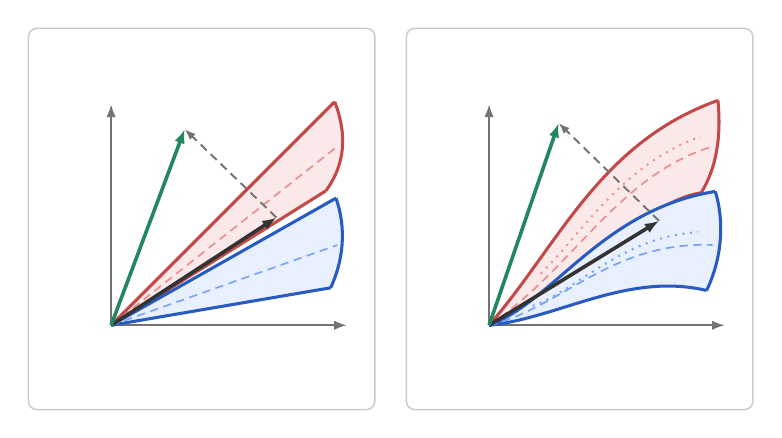
\begin{tikzpicture}
    \ifdefined\ONLYB
        \panelB
    \else
        \ifdefined\ONLYC
            \panelC
        \else
            \panelB
            \begin{scope}[xshift=4.80cm]
                \panelC
            \end{scope}
        \fi
    \fi
\end{tikzpicture}
\end{document}
'
%    xelatex -jobname=fig1_c_clean  '\def\ONLYC{}% ---------------------------------------------------------------------------
%  Figure 1 panels (b) and (c) -- TEXT-FREE export for PowerPoint.
%
%  Every label / annotation has been removed (panel titles, axis labels,
%  "$v_t^{cand}$", "$R_{1,\eta}$", "$VO^T_1$", origin "0", correction symbols,
%  the union equations ...).  Geometry, colours and line weights are identical
%  to the in-paper TikZ figure, so text can be re-added by hand in PPT.
%
%  Build from this folder:
%    xelatex -jobname=fig1_b_clean  '\def\ONLYB{}\input{fig1_bc_clean.tex}'
%    xelatex -jobname=fig1_c_clean  '\def\ONLYC{}\input{fig1_bc_clean.tex}'
%    xelatex -jobname=fig1_bc_clean '\input{fig1_bc_clean.tex}'
% ---------------------------------------------------------------------------
\documentclass[tikz,border=2pt]{standalone}

\usepackage{tikz}
\usetikzlibrary{arrows.meta,positioning,calc}

\definecolor{pvoBlue}{HTML}{2F6FED}
\definecolor{pvoGreen}{HTML}{2AA876}
\definecolor{pvoRed}{HTML}{E05252}

\tikzset{
    line join=round, line cap=round,
    panel/.style={rounded corners=3pt, draw=black!20, line width=0.55pt},
    axis/.style={-{Latex[length=1.6mm]}, line width=0.7pt, draw=black!55},
    riskone/.style={line width=1.1pt, draw=pvoRed!88!black},
    risktwo/.style={line width=1.1pt, draw=pvoBlue!82!black},
    meanline/.style={line width=0.62pt, densely dashed},
    candidate/.style={-{Latex[length=1.8mm]}, line width=1.3pt, draw=black!80},
    accepted/.style={-{Latex[length=1.8mm]}, line width=1.3pt, draw=pvoGreen!80!black},
    correction/.style={-{Latex[length=1.4mm]}, line width=0.7pt, densely dashed, draw=black!55}
}

% --------------------------------------------------------------- panel (b) --
\newcommand{\panelB}{%
    \draw[panel] (-0.10,-0.12) rectangle (4.30,4.72);
    \begin{scope}[shift={(0.95,0.95)}, scale=0.85, shift={(-0.48,-0.52)}]
        \draw[axis] (0.48,0.52) -- (4.00,0.52);
        \draw[axis] (0.48,0.52) -- (0.48,3.82);

        % deterministic relative-velocity cone for obstacle 1
        \path[fill=pvoRed!13]
            (0.48,0.52) -- (3.82,3.86)
            .. controls (4.01,3.37) and (3.98,2.93) .. (3.69,2.53) -- cycle;
        \draw[riskone] (0.48,0.52) -- (3.82,3.86);
        \draw[riskone] (0.48,0.52) -- (3.69,2.53);
        \draw[riskone] (3.82,3.86) .. controls (4.01,3.37) and (3.98,2.93) .. (3.69,2.53);
        \draw[meanline, pvoRed!64] (0.48,0.52) -- (3.82,3.16);

        % deterministic relative-velocity cone for obstacle 2
        \path[fill=pvoBlue!11]
            (0.48,0.52) -- (3.84,2.42)
            .. controls (4.00,1.96) and (3.95,1.49) .. (3.76,1.08) -- cycle;
        \draw[risktwo] (0.48,0.52) -- (3.84,2.42);
        \draw[risktwo] (0.48,0.52) -- (3.76,1.08);
        \draw[risktwo] (3.84,2.42) .. controls (4.00,1.96) and (3.95,1.49) .. (3.76,1.08);
        \draw[meanline, pvoBlue!62] (0.48,0.52) -- (3.86,1.72);

        % candidate velocity / filtered velocity / correction
        \draw[candidate] (0.48,0.52) -- (2.95,2.13);
        \draw[accepted] (0.48,0.52) -- (1.58,3.45);
        \draw[correction] (2.95,2.13) -- (1.58,3.45);
    \end{scope}%
}

% --------------------------------------------------------------- panel (c) --
\newcommand{\panelC}{%
    \draw[panel] (-0.10,-0.12) rectangle (4.30,4.72);
    \begin{scope}[shift={(0.95,0.95)}, scale=0.85, shift={(-0.48,-0.52)}]
        \draw[axis] (0.48,0.52) -- (4.00,0.52);
        \draw[axis] (0.48,0.52) -- (0.48,3.82);

        % action-conditioned risk tube for obstacle 1
        \path[fill=pvoRed!13]
            (0.48,0.52)
            .. controls (1.52,1.72) and (2.13,3.25) .. (3.90,3.88)
            .. controls (3.95,3.33) and (3.88,2.88) .. (3.65,2.50)
            .. controls (2.72,2.35) and (1.64,1.02) .. (0.48,0.52) -- cycle;
        \draw[riskone]
            (0.48,0.52) .. controls (1.52,1.72) and (2.13,3.25) .. (3.90,3.88);
        \draw[riskone]
            (0.48,0.52) .. controls (1.64,1.02) and (2.72,2.35) .. (3.65,2.50);
        \draw[riskone] (3.90,3.88) .. controls (3.95,3.33) and (3.88,2.88) .. (3.65,2.50);
        \draw[meanline, pvoRed!65]
            (0.48,0.52) .. controls (1.72,1.35) and (2.38,2.73) .. (3.78,3.18);
        \draw[dotted, line width=0.75pt, pvoRed!62]
            (1.25,1.29) .. controls (1.86,1.88) and (2.46,2.92) .. (3.64,3.34);

        % action-conditioned risk tube for obstacle 2
        \path[fill=pvoBlue!11]
            (0.48,0.52)
            .. controls (1.45,0.88) and (2.17,2.25) .. (3.86,2.52)
            .. controls (4.00,2.06) and (3.96,1.52) .. (3.73,1.04)
            .. controls (2.55,1.32) and (1.53,0.63) .. (0.48,0.52) -- cycle;
        \draw[risktwo]
            (0.48,0.52) .. controls (1.45,0.88) and (2.17,2.25) .. (3.86,2.52);
        \draw[risktwo]
            (0.48,0.52) .. controls (1.53,0.63) and (2.55,1.32) .. (3.73,1.04);
        \draw[risktwo] (3.86,2.52) .. controls (4.00,2.06) and (3.96,1.52) .. (3.73,1.04);
        \draw[meanline, pvoBlue!64]
            (0.48,0.52) .. controls (1.55,0.77) and (2.30,1.78) .. (3.82,1.72);
        \draw[dotted, line width=0.75pt, pvoBlue!62]
            (1.13,0.81) .. controls (1.79,1.04) and (2.48,1.85) .. (3.60,1.91);

        % candidate velocity / filtered velocity / correction
        \draw[candidate] (0.48,0.52) -- (3.02,2.08);
        \draw[accepted] (0.48,0.52) -- (1.52,3.54);
        \draw[correction] (3.02,2.08) -- (1.52,3.54);
    \end{scope}%
}

\begin{document}
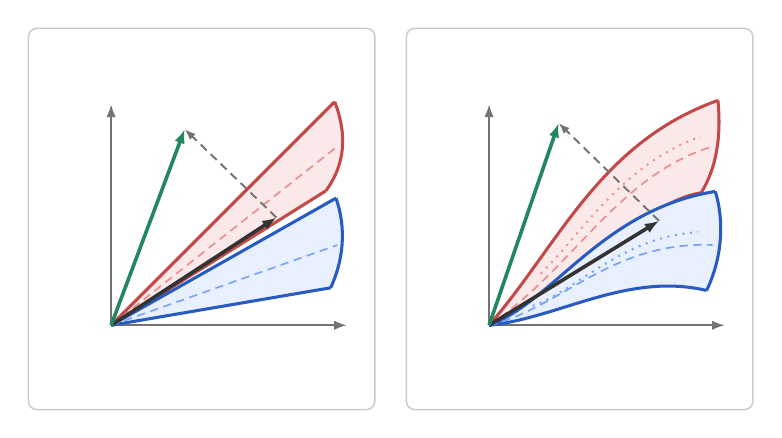
\begin{tikzpicture}
    \ifdefined\ONLYB
        \panelB
    \else
        \ifdefined\ONLYC
            \panelC
        \else
            \panelB
            \begin{scope}[xshift=4.80cm]
                \panelC
            \end{scope}
        \fi
    \fi
\end{tikzpicture}
\end{document}
'
%    xelatex -jobname=fig1_bc_clean '% ---------------------------------------------------------------------------
%  Figure 1 panels (b) and (c) -- TEXT-FREE export for PowerPoint.
%
%  Every label / annotation has been removed (panel titles, axis labels,
%  "$v_t^{cand}$", "$R_{1,\eta}$", "$VO^T_1$", origin "0", correction symbols,
%  the union equations ...).  Geometry, colours and line weights are identical
%  to the in-paper TikZ figure, so text can be re-added by hand in PPT.
%
%  Build from this folder:
%    xelatex -jobname=fig1_b_clean  '\def\ONLYB{}\input{fig1_bc_clean.tex}'
%    xelatex -jobname=fig1_c_clean  '\def\ONLYC{}\input{fig1_bc_clean.tex}'
%    xelatex -jobname=fig1_bc_clean '\input{fig1_bc_clean.tex}'
% ---------------------------------------------------------------------------
\documentclass[tikz,border=2pt]{standalone}

\usepackage{tikz}
\usetikzlibrary{arrows.meta,positioning,calc}

\definecolor{pvoBlue}{HTML}{2F6FED}
\definecolor{pvoGreen}{HTML}{2AA876}
\definecolor{pvoRed}{HTML}{E05252}

\tikzset{
    line join=round, line cap=round,
    panel/.style={rounded corners=3pt, draw=black!20, line width=0.55pt},
    axis/.style={-{Latex[length=1.6mm]}, line width=0.7pt, draw=black!55},
    riskone/.style={line width=1.1pt, draw=pvoRed!88!black},
    risktwo/.style={line width=1.1pt, draw=pvoBlue!82!black},
    meanline/.style={line width=0.62pt, densely dashed},
    candidate/.style={-{Latex[length=1.8mm]}, line width=1.3pt, draw=black!80},
    accepted/.style={-{Latex[length=1.8mm]}, line width=1.3pt, draw=pvoGreen!80!black},
    correction/.style={-{Latex[length=1.4mm]}, line width=0.7pt, densely dashed, draw=black!55}
}

% --------------------------------------------------------------- panel (b) --
\newcommand{\panelB}{%
    \draw[panel] (-0.10,-0.12) rectangle (4.30,4.72);
    \begin{scope}[shift={(0.95,0.95)}, scale=0.85, shift={(-0.48,-0.52)}]
        \draw[axis] (0.48,0.52) -- (4.00,0.52);
        \draw[axis] (0.48,0.52) -- (0.48,3.82);

        % deterministic relative-velocity cone for obstacle 1
        \path[fill=pvoRed!13]
            (0.48,0.52) -- (3.82,3.86)
            .. controls (4.01,3.37) and (3.98,2.93) .. (3.69,2.53) -- cycle;
        \draw[riskone] (0.48,0.52) -- (3.82,3.86);
        \draw[riskone] (0.48,0.52) -- (3.69,2.53);
        \draw[riskone] (3.82,3.86) .. controls (4.01,3.37) and (3.98,2.93) .. (3.69,2.53);
        \draw[meanline, pvoRed!64] (0.48,0.52) -- (3.82,3.16);

        % deterministic relative-velocity cone for obstacle 2
        \path[fill=pvoBlue!11]
            (0.48,0.52) -- (3.84,2.42)
            .. controls (4.00,1.96) and (3.95,1.49) .. (3.76,1.08) -- cycle;
        \draw[risktwo] (0.48,0.52) -- (3.84,2.42);
        \draw[risktwo] (0.48,0.52) -- (3.76,1.08);
        \draw[risktwo] (3.84,2.42) .. controls (4.00,1.96) and (3.95,1.49) .. (3.76,1.08);
        \draw[meanline, pvoBlue!62] (0.48,0.52) -- (3.86,1.72);

        % candidate velocity / filtered velocity / correction
        \draw[candidate] (0.48,0.52) -- (2.95,2.13);
        \draw[accepted] (0.48,0.52) -- (1.58,3.45);
        \draw[correction] (2.95,2.13) -- (1.58,3.45);
    \end{scope}%
}

% --------------------------------------------------------------- panel (c) --
\newcommand{\panelC}{%
    \draw[panel] (-0.10,-0.12) rectangle (4.30,4.72);
    \begin{scope}[shift={(0.95,0.95)}, scale=0.85, shift={(-0.48,-0.52)}]
        \draw[axis] (0.48,0.52) -- (4.00,0.52);
        \draw[axis] (0.48,0.52) -- (0.48,3.82);

        % action-conditioned risk tube for obstacle 1
        \path[fill=pvoRed!13]
            (0.48,0.52)
            .. controls (1.52,1.72) and (2.13,3.25) .. (3.90,3.88)
            .. controls (3.95,3.33) and (3.88,2.88) .. (3.65,2.50)
            .. controls (2.72,2.35) and (1.64,1.02) .. (0.48,0.52) -- cycle;
        \draw[riskone]
            (0.48,0.52) .. controls (1.52,1.72) and (2.13,3.25) .. (3.90,3.88);
        \draw[riskone]
            (0.48,0.52) .. controls (1.64,1.02) and (2.72,2.35) .. (3.65,2.50);
        \draw[riskone] (3.90,3.88) .. controls (3.95,3.33) and (3.88,2.88) .. (3.65,2.50);
        \draw[meanline, pvoRed!65]
            (0.48,0.52) .. controls (1.72,1.35) and (2.38,2.73) .. (3.78,3.18);
        \draw[dotted, line width=0.75pt, pvoRed!62]
            (1.25,1.29) .. controls (1.86,1.88) and (2.46,2.92) .. (3.64,3.34);

        % action-conditioned risk tube for obstacle 2
        \path[fill=pvoBlue!11]
            (0.48,0.52)
            .. controls (1.45,0.88) and (2.17,2.25) .. (3.86,2.52)
            .. controls (4.00,2.06) and (3.96,1.52) .. (3.73,1.04)
            .. controls (2.55,1.32) and (1.53,0.63) .. (0.48,0.52) -- cycle;
        \draw[risktwo]
            (0.48,0.52) .. controls (1.45,0.88) and (2.17,2.25) .. (3.86,2.52);
        \draw[risktwo]
            (0.48,0.52) .. controls (1.53,0.63) and (2.55,1.32) .. (3.73,1.04);
        \draw[risktwo] (3.86,2.52) .. controls (4.00,2.06) and (3.96,1.52) .. (3.73,1.04);
        \draw[meanline, pvoBlue!64]
            (0.48,0.52) .. controls (1.55,0.77) and (2.30,1.78) .. (3.82,1.72);
        \draw[dotted, line width=0.75pt, pvoBlue!62]
            (1.13,0.81) .. controls (1.79,1.04) and (2.48,1.85) .. (3.60,1.91);

        % candidate velocity / filtered velocity / correction
        \draw[candidate] (0.48,0.52) -- (3.02,2.08);
        \draw[accepted] (0.48,0.52) -- (1.52,3.54);
        \draw[correction] (3.02,2.08) -- (1.52,3.54);
    \end{scope}%
}

\begin{document}
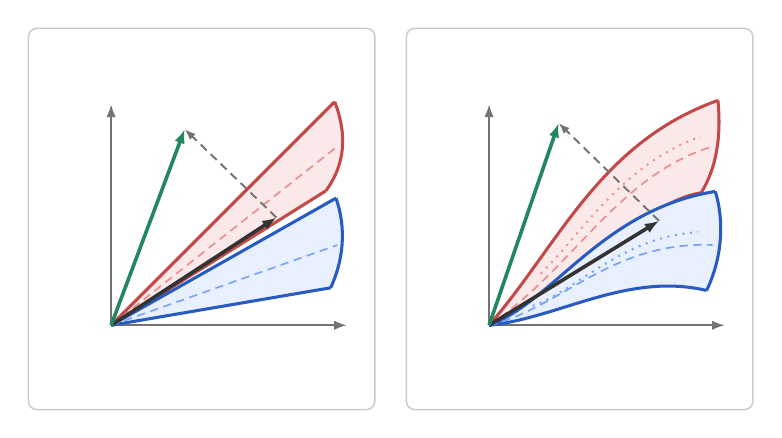
\begin{tikzpicture}
    \ifdefined\ONLYB
        \panelB
    \else
        \ifdefined\ONLYC
            \panelC
        \else
            \panelB
            \begin{scope}[xshift=4.80cm]
                \panelC
            \end{scope}
        \fi
    \fi
\end{tikzpicture}
\end{document}
'
% ---------------------------------------------------------------------------
\documentclass[tikz,border=2pt]{standalone}

\usepackage{tikz}
\usetikzlibrary{arrows.meta,positioning,calc}

\definecolor{pvoBlue}{HTML}{2F6FED}
\definecolor{pvoGreen}{HTML}{2AA876}
\definecolor{pvoRed}{HTML}{E05252}

\tikzset{
    line join=round, line cap=round,
    panel/.style={rounded corners=3pt, draw=black!20, line width=0.55pt},
    axis/.style={-{Latex[length=1.6mm]}, line width=0.7pt, draw=black!55},
    riskone/.style={line width=1.1pt, draw=pvoRed!88!black},
    risktwo/.style={line width=1.1pt, draw=pvoBlue!82!black},
    meanline/.style={line width=0.62pt, densely dashed},
    candidate/.style={-{Latex[length=1.8mm]}, line width=1.3pt, draw=black!80},
    accepted/.style={-{Latex[length=1.8mm]}, line width=1.3pt, draw=pvoGreen!80!black},
    correction/.style={-{Latex[length=1.4mm]}, line width=0.7pt, densely dashed, draw=black!55}
}

% --------------------------------------------------------------- panel (b) --
\newcommand{\panelB}{%
    \draw[panel] (-0.10,-0.12) rectangle (4.30,4.72);
    \begin{scope}[shift={(0.95,0.95)}, scale=0.85, shift={(-0.48,-0.52)}]
        \draw[axis] (0.48,0.52) -- (4.00,0.52);
        \draw[axis] (0.48,0.52) -- (0.48,3.82);

        % deterministic relative-velocity cone for obstacle 1
        \path[fill=pvoRed!13]
            (0.48,0.52) -- (3.82,3.86)
            .. controls (4.01,3.37) and (3.98,2.93) .. (3.69,2.53) -- cycle;
        \draw[riskone] (0.48,0.52) -- (3.82,3.86);
        \draw[riskone] (0.48,0.52) -- (3.69,2.53);
        \draw[riskone] (3.82,3.86) .. controls (4.01,3.37) and (3.98,2.93) .. (3.69,2.53);
        \draw[meanline, pvoRed!64] (0.48,0.52) -- (3.82,3.16);

        % deterministic relative-velocity cone for obstacle 2
        \path[fill=pvoBlue!11]
            (0.48,0.52) -- (3.84,2.42)
            .. controls (4.00,1.96) and (3.95,1.49) .. (3.76,1.08) -- cycle;
        \draw[risktwo] (0.48,0.52) -- (3.84,2.42);
        \draw[risktwo] (0.48,0.52) -- (3.76,1.08);
        \draw[risktwo] (3.84,2.42) .. controls (4.00,1.96) and (3.95,1.49) .. (3.76,1.08);
        \draw[meanline, pvoBlue!62] (0.48,0.52) -- (3.86,1.72);

        % candidate velocity / filtered velocity / correction
        \draw[candidate] (0.48,0.52) -- (2.95,2.13);
        \draw[accepted] (0.48,0.52) -- (1.58,3.45);
        \draw[correction] (2.95,2.13) -- (1.58,3.45);
    \end{scope}%
}

% --------------------------------------------------------------- panel (c) --
\newcommand{\panelC}{%
    \draw[panel] (-0.10,-0.12) rectangle (4.30,4.72);
    \begin{scope}[shift={(0.95,0.95)}, scale=0.85, shift={(-0.48,-0.52)}]
        \draw[axis] (0.48,0.52) -- (4.00,0.52);
        \draw[axis] (0.48,0.52) -- (0.48,3.82);

        % action-conditioned risk tube for obstacle 1
        \path[fill=pvoRed!13]
            (0.48,0.52)
            .. controls (1.52,1.72) and (2.13,3.25) .. (3.90,3.88)
            .. controls (3.95,3.33) and (3.88,2.88) .. (3.65,2.50)
            .. controls (2.72,2.35) and (1.64,1.02) .. (0.48,0.52) -- cycle;
        \draw[riskone]
            (0.48,0.52) .. controls (1.52,1.72) and (2.13,3.25) .. (3.90,3.88);
        \draw[riskone]
            (0.48,0.52) .. controls (1.64,1.02) and (2.72,2.35) .. (3.65,2.50);
        \draw[riskone] (3.90,3.88) .. controls (3.95,3.33) and (3.88,2.88) .. (3.65,2.50);
        \draw[meanline, pvoRed!65]
            (0.48,0.52) .. controls (1.72,1.35) and (2.38,2.73) .. (3.78,3.18);
        \draw[dotted, line width=0.75pt, pvoRed!62]
            (1.25,1.29) .. controls (1.86,1.88) and (2.46,2.92) .. (3.64,3.34);

        % action-conditioned risk tube for obstacle 2
        \path[fill=pvoBlue!11]
            (0.48,0.52)
            .. controls (1.45,0.88) and (2.17,2.25) .. (3.86,2.52)
            .. controls (4.00,2.06) and (3.96,1.52) .. (3.73,1.04)
            .. controls (2.55,1.32) and (1.53,0.63) .. (0.48,0.52) -- cycle;
        \draw[risktwo]
            (0.48,0.52) .. controls (1.45,0.88) and (2.17,2.25) .. (3.86,2.52);
        \draw[risktwo]
            (0.48,0.52) .. controls (1.53,0.63) and (2.55,1.32) .. (3.73,1.04);
        \draw[risktwo] (3.86,2.52) .. controls (4.00,2.06) and (3.96,1.52) .. (3.73,1.04);
        \draw[meanline, pvoBlue!64]
            (0.48,0.52) .. controls (1.55,0.77) and (2.30,1.78) .. (3.82,1.72);
        \draw[dotted, line width=0.75pt, pvoBlue!62]
            (1.13,0.81) .. controls (1.79,1.04) and (2.48,1.85) .. (3.60,1.91);

        % candidate velocity / filtered velocity / correction
        \draw[candidate] (0.48,0.52) -- (3.02,2.08);
        \draw[accepted] (0.48,0.52) -- (1.52,3.54);
        \draw[correction] (3.02,2.08) -- (1.52,3.54);
    \end{scope}%
}

\begin{document}
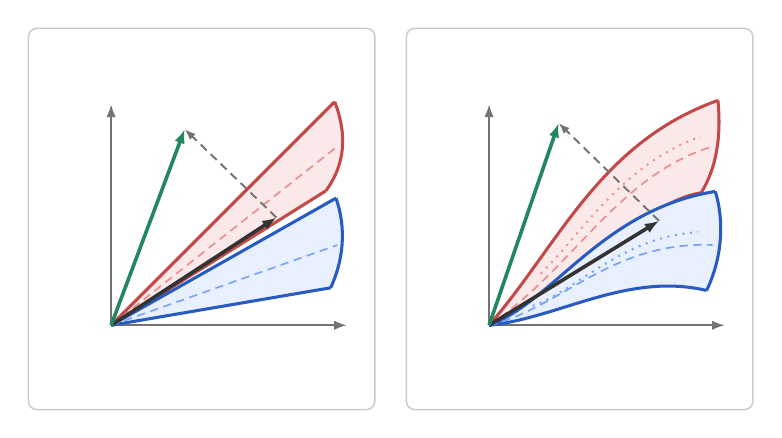
\begin{tikzpicture}
    \ifdefined\ONLYB
        \panelB
    \else
        \ifdefined\ONLYC
            \panelC
        \else
            \panelB
            \begin{scope}[xshift=4.80cm]
                \panelC
            \end{scope}
        \fi
    \fi
\end{tikzpicture}
\end{document}
'
%    xelatex -jobname=fig1_bc_clean '% ---------------------------------------------------------------------------
%  Figure 1 panels (b) and (c) -- TEXT-FREE export for PowerPoint.
%
%  Every label / annotation has been removed (panel titles, axis labels,
%  "$v_t^{cand}$", "$R_{1,\eta}$", "$VO^T_1$", origin "0", correction symbols,
%  the union equations ...).  Geometry, colours and line weights are identical
%  to the in-paper TikZ figure, so text can be re-added by hand in PPT.
%
%  Build from this folder:
%    xelatex -jobname=fig1_b_clean  '\def\ONLYB{}% ---------------------------------------------------------------------------
%  Figure 1 panels (b) and (c) -- TEXT-FREE export for PowerPoint.
%
%  Every label / annotation has been removed (panel titles, axis labels,
%  "$v_t^{cand}$", "$R_{1,\eta}$", "$VO^T_1$", origin "0", correction symbols,
%  the union equations ...).  Geometry, colours and line weights are identical
%  to the in-paper TikZ figure, so text can be re-added by hand in PPT.
%
%  Build from this folder:
%    xelatex -jobname=fig1_b_clean  '\def\ONLYB{}\input{fig1_bc_clean.tex}'
%    xelatex -jobname=fig1_c_clean  '\def\ONLYC{}\input{fig1_bc_clean.tex}'
%    xelatex -jobname=fig1_bc_clean '\input{fig1_bc_clean.tex}'
% ---------------------------------------------------------------------------
\documentclass[tikz,border=2pt]{standalone}

\usepackage{tikz}
\usetikzlibrary{arrows.meta,positioning,calc}

\definecolor{pvoBlue}{HTML}{2F6FED}
\definecolor{pvoGreen}{HTML}{2AA876}
\definecolor{pvoRed}{HTML}{E05252}

\tikzset{
    line join=round, line cap=round,
    panel/.style={rounded corners=3pt, draw=black!20, line width=0.55pt},
    axis/.style={-{Latex[length=1.6mm]}, line width=0.7pt, draw=black!55},
    riskone/.style={line width=1.1pt, draw=pvoRed!88!black},
    risktwo/.style={line width=1.1pt, draw=pvoBlue!82!black},
    meanline/.style={line width=0.62pt, densely dashed},
    candidate/.style={-{Latex[length=1.8mm]}, line width=1.3pt, draw=black!80},
    accepted/.style={-{Latex[length=1.8mm]}, line width=1.3pt, draw=pvoGreen!80!black},
    correction/.style={-{Latex[length=1.4mm]}, line width=0.7pt, densely dashed, draw=black!55}
}

% --------------------------------------------------------------- panel (b) --
\newcommand{\panelB}{%
    \draw[panel] (-0.10,-0.12) rectangle (4.30,4.72);
    \begin{scope}[shift={(0.95,0.95)}, scale=0.85, shift={(-0.48,-0.52)}]
        \draw[axis] (0.48,0.52) -- (4.00,0.52);
        \draw[axis] (0.48,0.52) -- (0.48,3.82);

        % deterministic relative-velocity cone for obstacle 1
        \path[fill=pvoRed!13]
            (0.48,0.52) -- (3.82,3.86)
            .. controls (4.01,3.37) and (3.98,2.93) .. (3.69,2.53) -- cycle;
        \draw[riskone] (0.48,0.52) -- (3.82,3.86);
        \draw[riskone] (0.48,0.52) -- (3.69,2.53);
        \draw[riskone] (3.82,3.86) .. controls (4.01,3.37) and (3.98,2.93) .. (3.69,2.53);
        \draw[meanline, pvoRed!64] (0.48,0.52) -- (3.82,3.16);

        % deterministic relative-velocity cone for obstacle 2
        \path[fill=pvoBlue!11]
            (0.48,0.52) -- (3.84,2.42)
            .. controls (4.00,1.96) and (3.95,1.49) .. (3.76,1.08) -- cycle;
        \draw[risktwo] (0.48,0.52) -- (3.84,2.42);
        \draw[risktwo] (0.48,0.52) -- (3.76,1.08);
        \draw[risktwo] (3.84,2.42) .. controls (4.00,1.96) and (3.95,1.49) .. (3.76,1.08);
        \draw[meanline, pvoBlue!62] (0.48,0.52) -- (3.86,1.72);

        % candidate velocity / filtered velocity / correction
        \draw[candidate] (0.48,0.52) -- (2.95,2.13);
        \draw[accepted] (0.48,0.52) -- (1.58,3.45);
        \draw[correction] (2.95,2.13) -- (1.58,3.45);
    \end{scope}%
}

% --------------------------------------------------------------- panel (c) --
\newcommand{\panelC}{%
    \draw[panel] (-0.10,-0.12) rectangle (4.30,4.72);
    \begin{scope}[shift={(0.95,0.95)}, scale=0.85, shift={(-0.48,-0.52)}]
        \draw[axis] (0.48,0.52) -- (4.00,0.52);
        \draw[axis] (0.48,0.52) -- (0.48,3.82);

        % action-conditioned risk tube for obstacle 1
        \path[fill=pvoRed!13]
            (0.48,0.52)
            .. controls (1.52,1.72) and (2.13,3.25) .. (3.90,3.88)
            .. controls (3.95,3.33) and (3.88,2.88) .. (3.65,2.50)
            .. controls (2.72,2.35) and (1.64,1.02) .. (0.48,0.52) -- cycle;
        \draw[riskone]
            (0.48,0.52) .. controls (1.52,1.72) and (2.13,3.25) .. (3.90,3.88);
        \draw[riskone]
            (0.48,0.52) .. controls (1.64,1.02) and (2.72,2.35) .. (3.65,2.50);
        \draw[riskone] (3.90,3.88) .. controls (3.95,3.33) and (3.88,2.88) .. (3.65,2.50);
        \draw[meanline, pvoRed!65]
            (0.48,0.52) .. controls (1.72,1.35) and (2.38,2.73) .. (3.78,3.18);
        \draw[dotted, line width=0.75pt, pvoRed!62]
            (1.25,1.29) .. controls (1.86,1.88) and (2.46,2.92) .. (3.64,3.34);

        % action-conditioned risk tube for obstacle 2
        \path[fill=pvoBlue!11]
            (0.48,0.52)
            .. controls (1.45,0.88) and (2.17,2.25) .. (3.86,2.52)
            .. controls (4.00,2.06) and (3.96,1.52) .. (3.73,1.04)
            .. controls (2.55,1.32) and (1.53,0.63) .. (0.48,0.52) -- cycle;
        \draw[risktwo]
            (0.48,0.52) .. controls (1.45,0.88) and (2.17,2.25) .. (3.86,2.52);
        \draw[risktwo]
            (0.48,0.52) .. controls (1.53,0.63) and (2.55,1.32) .. (3.73,1.04);
        \draw[risktwo] (3.86,2.52) .. controls (4.00,2.06) and (3.96,1.52) .. (3.73,1.04);
        \draw[meanline, pvoBlue!64]
            (0.48,0.52) .. controls (1.55,0.77) and (2.30,1.78) .. (3.82,1.72);
        \draw[dotted, line width=0.75pt, pvoBlue!62]
            (1.13,0.81) .. controls (1.79,1.04) and (2.48,1.85) .. (3.60,1.91);

        % candidate velocity / filtered velocity / correction
        \draw[candidate] (0.48,0.52) -- (3.02,2.08);
        \draw[accepted] (0.48,0.52) -- (1.52,3.54);
        \draw[correction] (3.02,2.08) -- (1.52,3.54);
    \end{scope}%
}

\begin{document}
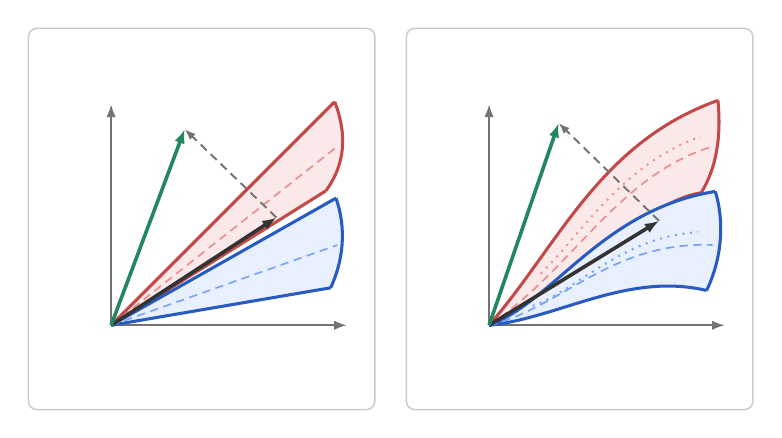
\begin{tikzpicture}
    \ifdefined\ONLYB
        \panelB
    \else
        \ifdefined\ONLYC
            \panelC
        \else
            \panelB
            \begin{scope}[xshift=4.80cm]
                \panelC
            \end{scope}
        \fi
    \fi
\end{tikzpicture}
\end{document}
'
%    xelatex -jobname=fig1_c_clean  '\def\ONLYC{}% ---------------------------------------------------------------------------
%  Figure 1 panels (b) and (c) -- TEXT-FREE export for PowerPoint.
%
%  Every label / annotation has been removed (panel titles, axis labels,
%  "$v_t^{cand}$", "$R_{1,\eta}$", "$VO^T_1$", origin "0", correction symbols,
%  the union equations ...).  Geometry, colours and line weights are identical
%  to the in-paper TikZ figure, so text can be re-added by hand in PPT.
%
%  Build from this folder:
%    xelatex -jobname=fig1_b_clean  '\def\ONLYB{}\input{fig1_bc_clean.tex}'
%    xelatex -jobname=fig1_c_clean  '\def\ONLYC{}\input{fig1_bc_clean.tex}'
%    xelatex -jobname=fig1_bc_clean '\input{fig1_bc_clean.tex}'
% ---------------------------------------------------------------------------
\documentclass[tikz,border=2pt]{standalone}

\usepackage{tikz}
\usetikzlibrary{arrows.meta,positioning,calc}

\definecolor{pvoBlue}{HTML}{2F6FED}
\definecolor{pvoGreen}{HTML}{2AA876}
\definecolor{pvoRed}{HTML}{E05252}

\tikzset{
    line join=round, line cap=round,
    panel/.style={rounded corners=3pt, draw=black!20, line width=0.55pt},
    axis/.style={-{Latex[length=1.6mm]}, line width=0.7pt, draw=black!55},
    riskone/.style={line width=1.1pt, draw=pvoRed!88!black},
    risktwo/.style={line width=1.1pt, draw=pvoBlue!82!black},
    meanline/.style={line width=0.62pt, densely dashed},
    candidate/.style={-{Latex[length=1.8mm]}, line width=1.3pt, draw=black!80},
    accepted/.style={-{Latex[length=1.8mm]}, line width=1.3pt, draw=pvoGreen!80!black},
    correction/.style={-{Latex[length=1.4mm]}, line width=0.7pt, densely dashed, draw=black!55}
}

% --------------------------------------------------------------- panel (b) --
\newcommand{\panelB}{%
    \draw[panel] (-0.10,-0.12) rectangle (4.30,4.72);
    \begin{scope}[shift={(0.95,0.95)}, scale=0.85, shift={(-0.48,-0.52)}]
        \draw[axis] (0.48,0.52) -- (4.00,0.52);
        \draw[axis] (0.48,0.52) -- (0.48,3.82);

        % deterministic relative-velocity cone for obstacle 1
        \path[fill=pvoRed!13]
            (0.48,0.52) -- (3.82,3.86)
            .. controls (4.01,3.37) and (3.98,2.93) .. (3.69,2.53) -- cycle;
        \draw[riskone] (0.48,0.52) -- (3.82,3.86);
        \draw[riskone] (0.48,0.52) -- (3.69,2.53);
        \draw[riskone] (3.82,3.86) .. controls (4.01,3.37) and (3.98,2.93) .. (3.69,2.53);
        \draw[meanline, pvoRed!64] (0.48,0.52) -- (3.82,3.16);

        % deterministic relative-velocity cone for obstacle 2
        \path[fill=pvoBlue!11]
            (0.48,0.52) -- (3.84,2.42)
            .. controls (4.00,1.96) and (3.95,1.49) .. (3.76,1.08) -- cycle;
        \draw[risktwo] (0.48,0.52) -- (3.84,2.42);
        \draw[risktwo] (0.48,0.52) -- (3.76,1.08);
        \draw[risktwo] (3.84,2.42) .. controls (4.00,1.96) and (3.95,1.49) .. (3.76,1.08);
        \draw[meanline, pvoBlue!62] (0.48,0.52) -- (3.86,1.72);

        % candidate velocity / filtered velocity / correction
        \draw[candidate] (0.48,0.52) -- (2.95,2.13);
        \draw[accepted] (0.48,0.52) -- (1.58,3.45);
        \draw[correction] (2.95,2.13) -- (1.58,3.45);
    \end{scope}%
}

% --------------------------------------------------------------- panel (c) --
\newcommand{\panelC}{%
    \draw[panel] (-0.10,-0.12) rectangle (4.30,4.72);
    \begin{scope}[shift={(0.95,0.95)}, scale=0.85, shift={(-0.48,-0.52)}]
        \draw[axis] (0.48,0.52) -- (4.00,0.52);
        \draw[axis] (0.48,0.52) -- (0.48,3.82);

        % action-conditioned risk tube for obstacle 1
        \path[fill=pvoRed!13]
            (0.48,0.52)
            .. controls (1.52,1.72) and (2.13,3.25) .. (3.90,3.88)
            .. controls (3.95,3.33) and (3.88,2.88) .. (3.65,2.50)
            .. controls (2.72,2.35) and (1.64,1.02) .. (0.48,0.52) -- cycle;
        \draw[riskone]
            (0.48,0.52) .. controls (1.52,1.72) and (2.13,3.25) .. (3.90,3.88);
        \draw[riskone]
            (0.48,0.52) .. controls (1.64,1.02) and (2.72,2.35) .. (3.65,2.50);
        \draw[riskone] (3.90,3.88) .. controls (3.95,3.33) and (3.88,2.88) .. (3.65,2.50);
        \draw[meanline, pvoRed!65]
            (0.48,0.52) .. controls (1.72,1.35) and (2.38,2.73) .. (3.78,3.18);
        \draw[dotted, line width=0.75pt, pvoRed!62]
            (1.25,1.29) .. controls (1.86,1.88) and (2.46,2.92) .. (3.64,3.34);

        % action-conditioned risk tube for obstacle 2
        \path[fill=pvoBlue!11]
            (0.48,0.52)
            .. controls (1.45,0.88) and (2.17,2.25) .. (3.86,2.52)
            .. controls (4.00,2.06) and (3.96,1.52) .. (3.73,1.04)
            .. controls (2.55,1.32) and (1.53,0.63) .. (0.48,0.52) -- cycle;
        \draw[risktwo]
            (0.48,0.52) .. controls (1.45,0.88) and (2.17,2.25) .. (3.86,2.52);
        \draw[risktwo]
            (0.48,0.52) .. controls (1.53,0.63) and (2.55,1.32) .. (3.73,1.04);
        \draw[risktwo] (3.86,2.52) .. controls (4.00,2.06) and (3.96,1.52) .. (3.73,1.04);
        \draw[meanline, pvoBlue!64]
            (0.48,0.52) .. controls (1.55,0.77) and (2.30,1.78) .. (3.82,1.72);
        \draw[dotted, line width=0.75pt, pvoBlue!62]
            (1.13,0.81) .. controls (1.79,1.04) and (2.48,1.85) .. (3.60,1.91);

        % candidate velocity / filtered velocity / correction
        \draw[candidate] (0.48,0.52) -- (3.02,2.08);
        \draw[accepted] (0.48,0.52) -- (1.52,3.54);
        \draw[correction] (3.02,2.08) -- (1.52,3.54);
    \end{scope}%
}

\begin{document}
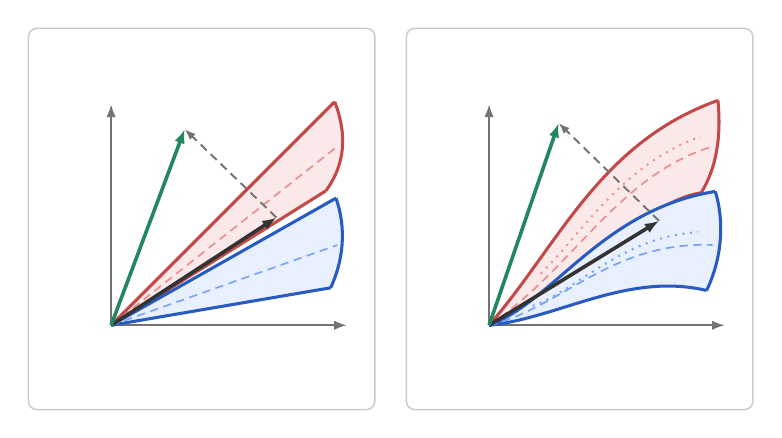
\begin{tikzpicture}
    \ifdefined\ONLYB
        \panelB
    \else
        \ifdefined\ONLYC
            \panelC
        \else
            \panelB
            \begin{scope}[xshift=4.80cm]
                \panelC
            \end{scope}
        \fi
    \fi
\end{tikzpicture}
\end{document}
'
%    xelatex -jobname=fig1_bc_clean '% ---------------------------------------------------------------------------
%  Figure 1 panels (b) and (c) -- TEXT-FREE export for PowerPoint.
%
%  Every label / annotation has been removed (panel titles, axis labels,
%  "$v_t^{cand}$", "$R_{1,\eta}$", "$VO^T_1$", origin "0", correction symbols,
%  the union equations ...).  Geometry, colours and line weights are identical
%  to the in-paper TikZ figure, so text can be re-added by hand in PPT.
%
%  Build from this folder:
%    xelatex -jobname=fig1_b_clean  '\def\ONLYB{}\input{fig1_bc_clean.tex}'
%    xelatex -jobname=fig1_c_clean  '\def\ONLYC{}\input{fig1_bc_clean.tex}'
%    xelatex -jobname=fig1_bc_clean '\input{fig1_bc_clean.tex}'
% ---------------------------------------------------------------------------
\documentclass[tikz,border=2pt]{standalone}

\usepackage{tikz}
\usetikzlibrary{arrows.meta,positioning,calc}

\definecolor{pvoBlue}{HTML}{2F6FED}
\definecolor{pvoGreen}{HTML}{2AA876}
\definecolor{pvoRed}{HTML}{E05252}

\tikzset{
    line join=round, line cap=round,
    panel/.style={rounded corners=3pt, draw=black!20, line width=0.55pt},
    axis/.style={-{Latex[length=1.6mm]}, line width=0.7pt, draw=black!55},
    riskone/.style={line width=1.1pt, draw=pvoRed!88!black},
    risktwo/.style={line width=1.1pt, draw=pvoBlue!82!black},
    meanline/.style={line width=0.62pt, densely dashed},
    candidate/.style={-{Latex[length=1.8mm]}, line width=1.3pt, draw=black!80},
    accepted/.style={-{Latex[length=1.8mm]}, line width=1.3pt, draw=pvoGreen!80!black},
    correction/.style={-{Latex[length=1.4mm]}, line width=0.7pt, densely dashed, draw=black!55}
}

% --------------------------------------------------------------- panel (b) --
\newcommand{\panelB}{%
    \draw[panel] (-0.10,-0.12) rectangle (4.30,4.72);
    \begin{scope}[shift={(0.95,0.95)}, scale=0.85, shift={(-0.48,-0.52)}]
        \draw[axis] (0.48,0.52) -- (4.00,0.52);
        \draw[axis] (0.48,0.52) -- (0.48,3.82);

        % deterministic relative-velocity cone for obstacle 1
        \path[fill=pvoRed!13]
            (0.48,0.52) -- (3.82,3.86)
            .. controls (4.01,3.37) and (3.98,2.93) .. (3.69,2.53) -- cycle;
        \draw[riskone] (0.48,0.52) -- (3.82,3.86);
        \draw[riskone] (0.48,0.52) -- (3.69,2.53);
        \draw[riskone] (3.82,3.86) .. controls (4.01,3.37) and (3.98,2.93) .. (3.69,2.53);
        \draw[meanline, pvoRed!64] (0.48,0.52) -- (3.82,3.16);

        % deterministic relative-velocity cone for obstacle 2
        \path[fill=pvoBlue!11]
            (0.48,0.52) -- (3.84,2.42)
            .. controls (4.00,1.96) and (3.95,1.49) .. (3.76,1.08) -- cycle;
        \draw[risktwo] (0.48,0.52) -- (3.84,2.42);
        \draw[risktwo] (0.48,0.52) -- (3.76,1.08);
        \draw[risktwo] (3.84,2.42) .. controls (4.00,1.96) and (3.95,1.49) .. (3.76,1.08);
        \draw[meanline, pvoBlue!62] (0.48,0.52) -- (3.86,1.72);

        % candidate velocity / filtered velocity / correction
        \draw[candidate] (0.48,0.52) -- (2.95,2.13);
        \draw[accepted] (0.48,0.52) -- (1.58,3.45);
        \draw[correction] (2.95,2.13) -- (1.58,3.45);
    \end{scope}%
}

% --------------------------------------------------------------- panel (c) --
\newcommand{\panelC}{%
    \draw[panel] (-0.10,-0.12) rectangle (4.30,4.72);
    \begin{scope}[shift={(0.95,0.95)}, scale=0.85, shift={(-0.48,-0.52)}]
        \draw[axis] (0.48,0.52) -- (4.00,0.52);
        \draw[axis] (0.48,0.52) -- (0.48,3.82);

        % action-conditioned risk tube for obstacle 1
        \path[fill=pvoRed!13]
            (0.48,0.52)
            .. controls (1.52,1.72) and (2.13,3.25) .. (3.90,3.88)
            .. controls (3.95,3.33) and (3.88,2.88) .. (3.65,2.50)
            .. controls (2.72,2.35) and (1.64,1.02) .. (0.48,0.52) -- cycle;
        \draw[riskone]
            (0.48,0.52) .. controls (1.52,1.72) and (2.13,3.25) .. (3.90,3.88);
        \draw[riskone]
            (0.48,0.52) .. controls (1.64,1.02) and (2.72,2.35) .. (3.65,2.50);
        \draw[riskone] (3.90,3.88) .. controls (3.95,3.33) and (3.88,2.88) .. (3.65,2.50);
        \draw[meanline, pvoRed!65]
            (0.48,0.52) .. controls (1.72,1.35) and (2.38,2.73) .. (3.78,3.18);
        \draw[dotted, line width=0.75pt, pvoRed!62]
            (1.25,1.29) .. controls (1.86,1.88) and (2.46,2.92) .. (3.64,3.34);

        % action-conditioned risk tube for obstacle 2
        \path[fill=pvoBlue!11]
            (0.48,0.52)
            .. controls (1.45,0.88) and (2.17,2.25) .. (3.86,2.52)
            .. controls (4.00,2.06) and (3.96,1.52) .. (3.73,1.04)
            .. controls (2.55,1.32) and (1.53,0.63) .. (0.48,0.52) -- cycle;
        \draw[risktwo]
            (0.48,0.52) .. controls (1.45,0.88) and (2.17,2.25) .. (3.86,2.52);
        \draw[risktwo]
            (0.48,0.52) .. controls (1.53,0.63) and (2.55,1.32) .. (3.73,1.04);
        \draw[risktwo] (3.86,2.52) .. controls (4.00,2.06) and (3.96,1.52) .. (3.73,1.04);
        \draw[meanline, pvoBlue!64]
            (0.48,0.52) .. controls (1.55,0.77) and (2.30,1.78) .. (3.82,1.72);
        \draw[dotted, line width=0.75pt, pvoBlue!62]
            (1.13,0.81) .. controls (1.79,1.04) and (2.48,1.85) .. (3.60,1.91);

        % candidate velocity / filtered velocity / correction
        \draw[candidate] (0.48,0.52) -- (3.02,2.08);
        \draw[accepted] (0.48,0.52) -- (1.52,3.54);
        \draw[correction] (3.02,2.08) -- (1.52,3.54);
    \end{scope}%
}

\begin{document}
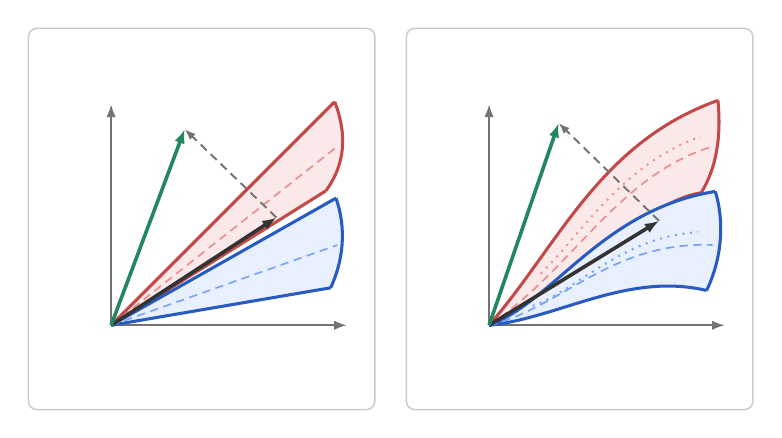
\begin{tikzpicture}
    \ifdefined\ONLYB
        \panelB
    \else
        \ifdefined\ONLYC
            \panelC
        \else
            \panelB
            \begin{scope}[xshift=4.80cm]
                \panelC
            \end{scope}
        \fi
    \fi
\end{tikzpicture}
\end{document}
'
% ---------------------------------------------------------------------------
\documentclass[tikz,border=2pt]{standalone}

\usepackage{tikz}
\usetikzlibrary{arrows.meta,positioning,calc}

\definecolor{pvoBlue}{HTML}{2F6FED}
\definecolor{pvoGreen}{HTML}{2AA876}
\definecolor{pvoRed}{HTML}{E05252}

\tikzset{
    line join=round, line cap=round,
    panel/.style={rounded corners=3pt, draw=black!20, line width=0.55pt},
    axis/.style={-{Latex[length=1.6mm]}, line width=0.7pt, draw=black!55},
    riskone/.style={line width=1.1pt, draw=pvoRed!88!black},
    risktwo/.style={line width=1.1pt, draw=pvoBlue!82!black},
    meanline/.style={line width=0.62pt, densely dashed},
    candidate/.style={-{Latex[length=1.8mm]}, line width=1.3pt, draw=black!80},
    accepted/.style={-{Latex[length=1.8mm]}, line width=1.3pt, draw=pvoGreen!80!black},
    correction/.style={-{Latex[length=1.4mm]}, line width=0.7pt, densely dashed, draw=black!55}
}

% --------------------------------------------------------------- panel (b) --
\newcommand{\panelB}{%
    \draw[panel] (-0.10,-0.12) rectangle (4.30,4.72);
    \begin{scope}[shift={(0.95,0.95)}, scale=0.85, shift={(-0.48,-0.52)}]
        \draw[axis] (0.48,0.52) -- (4.00,0.52);
        \draw[axis] (0.48,0.52) -- (0.48,3.82);

        % deterministic relative-velocity cone for obstacle 1
        \path[fill=pvoRed!13]
            (0.48,0.52) -- (3.82,3.86)
            .. controls (4.01,3.37) and (3.98,2.93) .. (3.69,2.53) -- cycle;
        \draw[riskone] (0.48,0.52) -- (3.82,3.86);
        \draw[riskone] (0.48,0.52) -- (3.69,2.53);
        \draw[riskone] (3.82,3.86) .. controls (4.01,3.37) and (3.98,2.93) .. (3.69,2.53);
        \draw[meanline, pvoRed!64] (0.48,0.52) -- (3.82,3.16);

        % deterministic relative-velocity cone for obstacle 2
        \path[fill=pvoBlue!11]
            (0.48,0.52) -- (3.84,2.42)
            .. controls (4.00,1.96) and (3.95,1.49) .. (3.76,1.08) -- cycle;
        \draw[risktwo] (0.48,0.52) -- (3.84,2.42);
        \draw[risktwo] (0.48,0.52) -- (3.76,1.08);
        \draw[risktwo] (3.84,2.42) .. controls (4.00,1.96) and (3.95,1.49) .. (3.76,1.08);
        \draw[meanline, pvoBlue!62] (0.48,0.52) -- (3.86,1.72);

        % candidate velocity / filtered velocity / correction
        \draw[candidate] (0.48,0.52) -- (2.95,2.13);
        \draw[accepted] (0.48,0.52) -- (1.58,3.45);
        \draw[correction] (2.95,2.13) -- (1.58,3.45);
    \end{scope}%
}

% --------------------------------------------------------------- panel (c) --
\newcommand{\panelC}{%
    \draw[panel] (-0.10,-0.12) rectangle (4.30,4.72);
    \begin{scope}[shift={(0.95,0.95)}, scale=0.85, shift={(-0.48,-0.52)}]
        \draw[axis] (0.48,0.52) -- (4.00,0.52);
        \draw[axis] (0.48,0.52) -- (0.48,3.82);

        % action-conditioned risk tube for obstacle 1
        \path[fill=pvoRed!13]
            (0.48,0.52)
            .. controls (1.52,1.72) and (2.13,3.25) .. (3.90,3.88)
            .. controls (3.95,3.33) and (3.88,2.88) .. (3.65,2.50)
            .. controls (2.72,2.35) and (1.64,1.02) .. (0.48,0.52) -- cycle;
        \draw[riskone]
            (0.48,0.52) .. controls (1.52,1.72) and (2.13,3.25) .. (3.90,3.88);
        \draw[riskone]
            (0.48,0.52) .. controls (1.64,1.02) and (2.72,2.35) .. (3.65,2.50);
        \draw[riskone] (3.90,3.88) .. controls (3.95,3.33) and (3.88,2.88) .. (3.65,2.50);
        \draw[meanline, pvoRed!65]
            (0.48,0.52) .. controls (1.72,1.35) and (2.38,2.73) .. (3.78,3.18);
        \draw[dotted, line width=0.75pt, pvoRed!62]
            (1.25,1.29) .. controls (1.86,1.88) and (2.46,2.92) .. (3.64,3.34);

        % action-conditioned risk tube for obstacle 2
        \path[fill=pvoBlue!11]
            (0.48,0.52)
            .. controls (1.45,0.88) and (2.17,2.25) .. (3.86,2.52)
            .. controls (4.00,2.06) and (3.96,1.52) .. (3.73,1.04)
            .. controls (2.55,1.32) and (1.53,0.63) .. (0.48,0.52) -- cycle;
        \draw[risktwo]
            (0.48,0.52) .. controls (1.45,0.88) and (2.17,2.25) .. (3.86,2.52);
        \draw[risktwo]
            (0.48,0.52) .. controls (1.53,0.63) and (2.55,1.32) .. (3.73,1.04);
        \draw[risktwo] (3.86,2.52) .. controls (4.00,2.06) and (3.96,1.52) .. (3.73,1.04);
        \draw[meanline, pvoBlue!64]
            (0.48,0.52) .. controls (1.55,0.77) and (2.30,1.78) .. (3.82,1.72);
        \draw[dotted, line width=0.75pt, pvoBlue!62]
            (1.13,0.81) .. controls (1.79,1.04) and (2.48,1.85) .. (3.60,1.91);

        % candidate velocity / filtered velocity / correction
        \draw[candidate] (0.48,0.52) -- (3.02,2.08);
        \draw[accepted] (0.48,0.52) -- (1.52,3.54);
        \draw[correction] (3.02,2.08) -- (1.52,3.54);
    \end{scope}%
}

\begin{document}
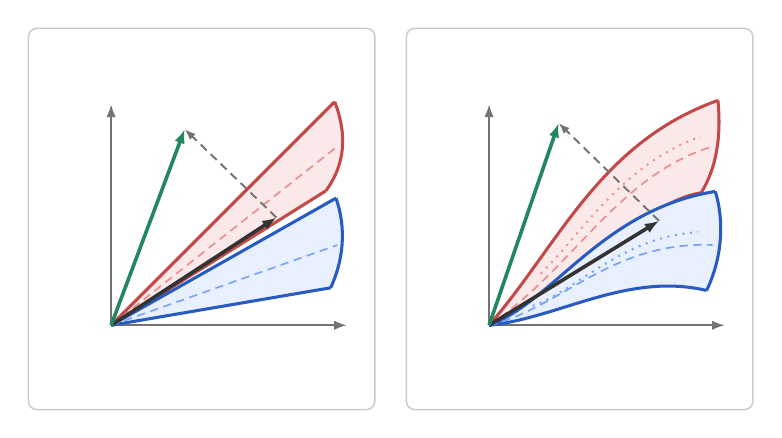
\begin{tikzpicture}
    \ifdefined\ONLYB
        \panelB
    \else
        \ifdefined\ONLYC
            \panelC
        \else
            \panelB
            \begin{scope}[xshift=4.80cm]
                \panelC
            \end{scope}
        \fi
    \fi
\end{tikzpicture}
\end{document}
'
% ---------------------------------------------------------------------------
\documentclass[tikz,border=2pt]{standalone}

\usepackage{tikz}
\usetikzlibrary{arrows.meta,positioning,calc}

\definecolor{pvoBlue}{HTML}{2F6FED}
\definecolor{pvoGreen}{HTML}{2AA876}
\definecolor{pvoRed}{HTML}{E05252}

\tikzset{
    line join=round, line cap=round,
    panel/.style={rounded corners=3pt, draw=black!20, line width=0.55pt},
    axis/.style={-{Latex[length=1.6mm]}, line width=0.7pt, draw=black!55},
    riskone/.style={line width=1.1pt, draw=pvoRed!88!black},
    risktwo/.style={line width=1.1pt, draw=pvoBlue!82!black},
    meanline/.style={line width=0.62pt, densely dashed},
    candidate/.style={-{Latex[length=1.8mm]}, line width=1.3pt, draw=black!80},
    accepted/.style={-{Latex[length=1.8mm]}, line width=1.3pt, draw=pvoGreen!80!black},
    correction/.style={-{Latex[length=1.4mm]}, line width=0.7pt, densely dashed, draw=black!55}
}

% --------------------------------------------------------------- panel (b) --
\newcommand{\panelB}{%
    \draw[panel] (-0.10,-0.12) rectangle (4.30,4.72);
    \begin{scope}[shift={(0.95,0.95)}, scale=0.85, shift={(-0.48,-0.52)}]
        \draw[axis] (0.48,0.52) -- (4.00,0.52);
        \draw[axis] (0.48,0.52) -- (0.48,3.82);

        % deterministic relative-velocity cone for obstacle 1
        \path[fill=pvoRed!13]
            (0.48,0.52) -- (3.82,3.86)
            .. controls (4.01,3.37) and (3.98,2.93) .. (3.69,2.53) -- cycle;
        \draw[riskone] (0.48,0.52) -- (3.82,3.86);
        \draw[riskone] (0.48,0.52) -- (3.69,2.53);
        \draw[riskone] (3.82,3.86) .. controls (4.01,3.37) and (3.98,2.93) .. (3.69,2.53);
        \draw[meanline, pvoRed!64] (0.48,0.52) -- (3.82,3.16);

        % deterministic relative-velocity cone for obstacle 2
        \path[fill=pvoBlue!11]
            (0.48,0.52) -- (3.84,2.42)
            .. controls (4.00,1.96) and (3.95,1.49) .. (3.76,1.08) -- cycle;
        \draw[risktwo] (0.48,0.52) -- (3.84,2.42);
        \draw[risktwo] (0.48,0.52) -- (3.76,1.08);
        \draw[risktwo] (3.84,2.42) .. controls (4.00,1.96) and (3.95,1.49) .. (3.76,1.08);
        \draw[meanline, pvoBlue!62] (0.48,0.52) -- (3.86,1.72);

        % candidate velocity / filtered velocity / correction
        \draw[candidate] (0.48,0.52) -- (2.95,2.13);
        \draw[accepted] (0.48,0.52) -- (1.58,3.45);
        \draw[correction] (2.95,2.13) -- (1.58,3.45);
    \end{scope}%
}

% --------------------------------------------------------------- panel (c) --
\newcommand{\panelC}{%
    \draw[panel] (-0.10,-0.12) rectangle (4.30,4.72);
    \begin{scope}[shift={(0.95,0.95)}, scale=0.85, shift={(-0.48,-0.52)}]
        \draw[axis] (0.48,0.52) -- (4.00,0.52);
        \draw[axis] (0.48,0.52) -- (0.48,3.82);

        % action-conditioned risk tube for obstacle 1
        \path[fill=pvoRed!13]
            (0.48,0.52)
            .. controls (1.52,1.72) and (2.13,3.25) .. (3.90,3.88)
            .. controls (3.95,3.33) and (3.88,2.88) .. (3.65,2.50)
            .. controls (2.72,2.35) and (1.64,1.02) .. (0.48,0.52) -- cycle;
        \draw[riskone]
            (0.48,0.52) .. controls (1.52,1.72) and (2.13,3.25) .. (3.90,3.88);
        \draw[riskone]
            (0.48,0.52) .. controls (1.64,1.02) and (2.72,2.35) .. (3.65,2.50);
        \draw[riskone] (3.90,3.88) .. controls (3.95,3.33) and (3.88,2.88) .. (3.65,2.50);
        \draw[meanline, pvoRed!65]
            (0.48,0.52) .. controls (1.72,1.35) and (2.38,2.73) .. (3.78,3.18);
        \draw[dotted, line width=0.75pt, pvoRed!62]
            (1.25,1.29) .. controls (1.86,1.88) and (2.46,2.92) .. (3.64,3.34);

        % action-conditioned risk tube for obstacle 2
        \path[fill=pvoBlue!11]
            (0.48,0.52)
            .. controls (1.45,0.88) and (2.17,2.25) .. (3.86,2.52)
            .. controls (4.00,2.06) and (3.96,1.52) .. (3.73,1.04)
            .. controls (2.55,1.32) and (1.53,0.63) .. (0.48,0.52) -- cycle;
        \draw[risktwo]
            (0.48,0.52) .. controls (1.45,0.88) and (2.17,2.25) .. (3.86,2.52);
        \draw[risktwo]
            (0.48,0.52) .. controls (1.53,0.63) and (2.55,1.32) .. (3.73,1.04);
        \draw[risktwo] (3.86,2.52) .. controls (4.00,2.06) and (3.96,1.52) .. (3.73,1.04);
        \draw[meanline, pvoBlue!64]
            (0.48,0.52) .. controls (1.55,0.77) and (2.30,1.78) .. (3.82,1.72);
        \draw[dotted, line width=0.75pt, pvoBlue!62]
            (1.13,0.81) .. controls (1.79,1.04) and (2.48,1.85) .. (3.60,1.91);

        % candidate velocity / filtered velocity / correction
        \draw[candidate] (0.48,0.52) -- (3.02,2.08);
        \draw[accepted] (0.48,0.52) -- (1.52,3.54);
        \draw[correction] (3.02,2.08) -- (1.52,3.54);
    \end{scope}%
}

\begin{document}
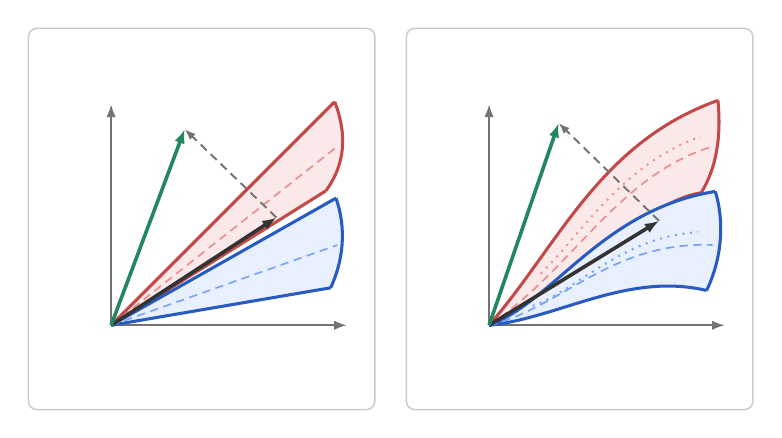
\begin{tikzpicture}
    \ifdefined\ONLYB
        \panelB
    \else
        \ifdefined\ONLYC
            \panelC
        \else
            \panelB
            \begin{scope}[xshift=4.80cm]
                \panelC
            \end{scope}
        \fi
    \fi
\end{tikzpicture}
\end{document}
'
% ---------------------------------------------------------------------------
\documentclass[tikz,border=2pt]{standalone}

\usepackage{tikz}
\usetikzlibrary{arrows.meta,positioning,calc}

\definecolor{pvoBlue}{HTML}{2F6FED}
\definecolor{pvoGreen}{HTML}{2AA876}
\definecolor{pvoRed}{HTML}{E05252}

\tikzset{
    line join=round, line cap=round,
    panel/.style={rounded corners=3pt, draw=black!20, line width=0.55pt},
    axis/.style={-{Latex[length=1.6mm]}, line width=0.7pt, draw=black!55},
    riskone/.style={line width=1.1pt, draw=pvoRed!88!black},
    risktwo/.style={line width=1.1pt, draw=pvoBlue!82!black},
    meanline/.style={line width=0.62pt, densely dashed},
    candidate/.style={-{Latex[length=1.8mm]}, line width=1.3pt, draw=black!80},
    accepted/.style={-{Latex[length=1.8mm]}, line width=1.3pt, draw=pvoGreen!80!black},
    correction/.style={-{Latex[length=1.4mm]}, line width=0.7pt, densely dashed, draw=black!55}
}

% --------------------------------------------------------------- panel (b) --
\newcommand{\panelB}{%
    \draw[panel] (-0.10,-0.12) rectangle (4.30,4.72);
    \begin{scope}[shift={(0.95,0.95)}, scale=0.85, shift={(-0.48,-0.52)}]
        \draw[axis] (0.48,0.52) -- (4.00,0.52);
        \draw[axis] (0.48,0.52) -- (0.48,3.82);

        % deterministic relative-velocity cone for obstacle 1
        \path[fill=pvoRed!13]
            (0.48,0.52) -- (3.82,3.86)
            .. controls (4.01,3.37) and (3.98,2.93) .. (3.69,2.53) -- cycle;
        \draw[riskone] (0.48,0.52) -- (3.82,3.86);
        \draw[riskone] (0.48,0.52) -- (3.69,2.53);
        \draw[riskone] (3.82,3.86) .. controls (4.01,3.37) and (3.98,2.93) .. (3.69,2.53);
        \draw[meanline, pvoRed!64] (0.48,0.52) -- (3.82,3.16);

        % deterministic relative-velocity cone for obstacle 2
        \path[fill=pvoBlue!11]
            (0.48,0.52) -- (3.84,2.42)
            .. controls (4.00,1.96) and (3.95,1.49) .. (3.76,1.08) -- cycle;
        \draw[risktwo] (0.48,0.52) -- (3.84,2.42);
        \draw[risktwo] (0.48,0.52) -- (3.76,1.08);
        \draw[risktwo] (3.84,2.42) .. controls (4.00,1.96) and (3.95,1.49) .. (3.76,1.08);
        \draw[meanline, pvoBlue!62] (0.48,0.52) -- (3.86,1.72);

        % candidate velocity / filtered velocity / correction
        \draw[candidate] (0.48,0.52) -- (2.95,2.13);
        \draw[accepted] (0.48,0.52) -- (1.58,3.45);
        \draw[correction] (2.95,2.13) -- (1.58,3.45);
    \end{scope}%
}

% --------------------------------------------------------------- panel (c) --
\newcommand{\panelC}{%
    \draw[panel] (-0.10,-0.12) rectangle (4.30,4.72);
    \begin{scope}[shift={(0.95,0.95)}, scale=0.85, shift={(-0.48,-0.52)}]
        \draw[axis] (0.48,0.52) -- (4.00,0.52);
        \draw[axis] (0.48,0.52) -- (0.48,3.82);

        % action-conditioned risk tube for obstacle 1
        \path[fill=pvoRed!13]
            (0.48,0.52)
            .. controls (1.52,1.72) and (2.13,3.25) .. (3.90,3.88)
            .. controls (3.95,3.33) and (3.88,2.88) .. (3.65,2.50)
            .. controls (2.72,2.35) and (1.64,1.02) .. (0.48,0.52) -- cycle;
        \draw[riskone]
            (0.48,0.52) .. controls (1.52,1.72) and (2.13,3.25) .. (3.90,3.88);
        \draw[riskone]
            (0.48,0.52) .. controls (1.64,1.02) and (2.72,2.35) .. (3.65,2.50);
        \draw[riskone] (3.90,3.88) .. controls (3.95,3.33) and (3.88,2.88) .. (3.65,2.50);
        \draw[meanline, pvoRed!65]
            (0.48,0.52) .. controls (1.72,1.35) and (2.38,2.73) .. (3.78,3.18);
        \draw[dotted, line width=0.75pt, pvoRed!62]
            (1.25,1.29) .. controls (1.86,1.88) and (2.46,2.92) .. (3.64,3.34);

        % action-conditioned risk tube for obstacle 2
        \path[fill=pvoBlue!11]
            (0.48,0.52)
            .. controls (1.45,0.88) and (2.17,2.25) .. (3.86,2.52)
            .. controls (4.00,2.06) and (3.96,1.52) .. (3.73,1.04)
            .. controls (2.55,1.32) and (1.53,0.63) .. (0.48,0.52) -- cycle;
        \draw[risktwo]
            (0.48,0.52) .. controls (1.45,0.88) and (2.17,2.25) .. (3.86,2.52);
        \draw[risktwo]
            (0.48,0.52) .. controls (1.53,0.63) and (2.55,1.32) .. (3.73,1.04);
        \draw[risktwo] (3.86,2.52) .. controls (4.00,2.06) and (3.96,1.52) .. (3.73,1.04);
        \draw[meanline, pvoBlue!64]
            (0.48,0.52) .. controls (1.55,0.77) and (2.30,1.78) .. (3.82,1.72);
        \draw[dotted, line width=0.75pt, pvoBlue!62]
            (1.13,0.81) .. controls (1.79,1.04) and (2.48,1.85) .. (3.60,1.91);

        % candidate velocity / filtered velocity / correction
        \draw[candidate] (0.48,0.52) -- (3.02,2.08);
        \draw[accepted] (0.48,0.52) -- (1.52,3.54);
        \draw[correction] (3.02,2.08) -- (1.52,3.54);
    \end{scope}%
}

\begin{document}
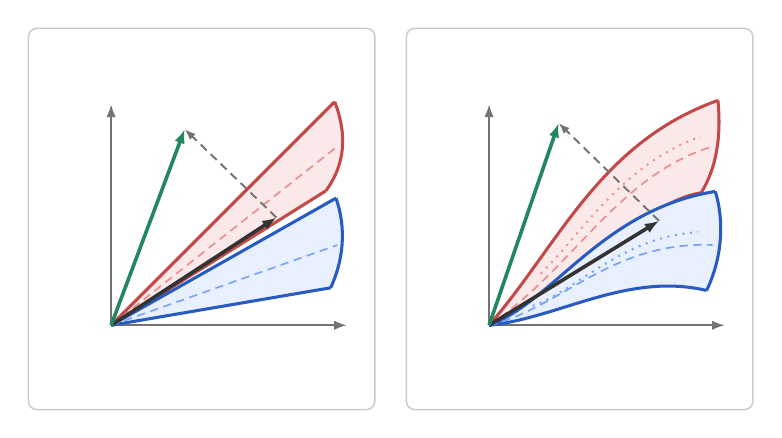
\begin{tikzpicture}
    \ifdefined\ONLYB
        \panelB
    \else
        \ifdefined\ONLYC
            \panelC
        \else
            \panelB
            \begin{scope}[xshift=4.80cm]
                \panelC
            \end{scope}
        \fi
    \fi
\end{tikzpicture}
\end{document}
